\documentclass[12pt]{article}
\usepackage[a4paper,margin = 30mm, right = 30mm]{geometry}
\usepackage[letterspace=150]{microtype}
\usepackage{graphics}
\usepackage{amsmath,latexsym, amssymb}
\usepackage{mathtools}
\usepackage{makecell}
\usepackage{nicematrix}
\usepackage{import}
\usepackage[english]{babel}
\usepackage{pgfpages}
\usepackage{fancyhdr}
\pagestyle{fancy}
\usepackage{bigints}
\usepackage{appendix}
\usepackage{esint}
\usepackage{caption}
\usepackage{subcaption}
\usepackage{tikz, tikz-3dplot}
\usepackage{braket}
\usepackage{multirow}
\usepackage[utf8]{inputenc}
\usetikzlibrary{calc,angles,quotes, intersections, babel}

\DeclareMathOperator{\arccosh}{arcosh}


\numberwithin{equation}{section}
\numberwithin{figure}{section}
\addto\captionsbulgarian{%
	\renewcommand\appendixname{Допълнение}
	\renewcommand\appendixpagename{Допълнения}
}

\cfoot{}

\fancyhead[R]{\thepage}

\begin{document}
	
	\thispagestyle{empty}
	\begin{center}
		
		\centering
		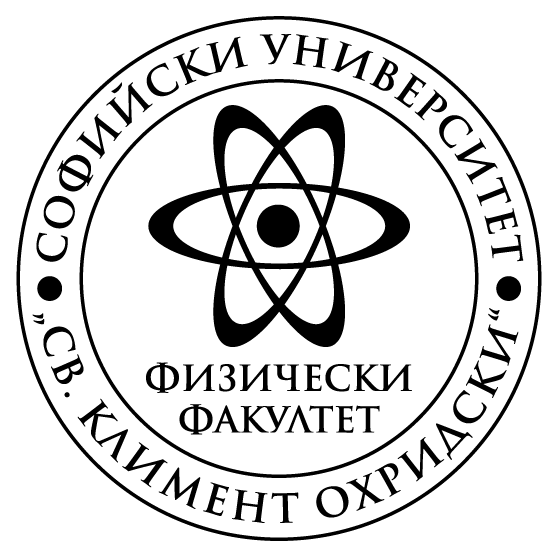
\includegraphics[scale = 1]{Title_page/logo-FzF.png}
		\noindent\makebox[\linewidth]{\rule{15cm}{0.8pt}}
		\textsc{Faculty of Physics}
		\noindent\makebox[\linewidth]{\rule{15cm}{0.8pt}}
		\textsc{Theoretical Physics Department}\\
		\bigskip
		\bigskip
		\bigskip
		\bigskip
		{\Large{\textbf{Valentin Olegov Deliyski}}}\\
		\bigskip
		\bigskip
		\bigskip
		{\Large \textbf{Optical effects in curved spacetime: gravitational lenses, shadows and the polarization of light}}\\
		\bigskip
		\bigskip
		\bigskip
		{\textbf{\huge \textls{ABSTRACT}}}\\
		\bigskip
		of the dissemination for acquiring the educational and scientific title "DOCTOR"\\
		\bigskip
		\bigskip
		\bigskip
		\textbf{Professional direction:} Physical sciences\\
		\textbf{Scientific specialty:} Theoretical and mathematical physics\\
		\bigskip
		\bigskip
		\bigskip
		\bigskip
		\textit{Supervisors:}\\
		Assoc Prof. Dr. Galin Gyulchev\\
		\bigskip
		Assoc. Mem. Acad. Sc. Prof. D.Sc. Stoytcho Yazadjiev\\
		\bigskip
		\textit{Scientific consultant:}\\
		Assoc Prof. Dr. Petya Nedkova\\
		
		\newpage
	\end{center}
	
	\nocite{EHT_M87_I,
		EHT_M87_II,
		EHT_M87_III,
		EHT_M87_IV,
		EHT_M87_V,
		EHT_M87_VI,
		EHT_M87_VII,
		EHT_M87_VIII,
		EHT_M87_IX,
		EHT_SGR_I,
		EHT_SGR_II,
		EHT_SGR_III,
		EHT_SGR_IV,
		EHT_SGR_V,
		EHT_SGR_VI,
		EHT_SGR_VII,
		EHT_SGR_VIII}
	
	\tableofcontents
	\listoffigures
	\listoftables
	\newpage
	
	\section{Introduction}
	
	The topic of this dissertation builds upon the results of the Event Horizon Telescope collaboration (EHT), which for the first time have managed to achieve the observational resolution, necessary to observe the immediate surroundings of the ultra-compact objects in the cores of the galaxies M87 and the Milky way \cite{EHT_M87_I} - \cite{EHT_SGR_VIII}. Similar future observational achievements will play a central role in probing the nature of gravity in the most extreme regimes. They can contribute to the experimental verification of additional fundamental fields, as well as the existence of \emph{exotic compact objects}, such as wormholes and naked singularities. Such object arise naturally in generalized theories of gravity, which makes their observation of fundamental importance.\\
	
	\emph{The goal of this dissertation is to examine the possibility of distinguishing such exotic compact objects from black holes via the current and future observational campaigns of the EHT collaboration.}\\
	
	\noindent More concretely, this dissertation focuses on the distinguishing signatures of these objects, which in general can manifest trough the following three observational features: the image morphology, its variability and polarization. They carry with them information about the nature of the compact object, as well as the theory that describes them, with the added complexity that it is non-linearly coupled to the magneto-hydrodynamics of the emission medium. This makes the interpretation of current and future observation a highly non-trivial problem and one of the main difficulties of studying such objects.\\
	
	\noindent Another difficulty is that a wide class of different exotic compact objects can have a qualitatively similar imprint on the observations. For example even though the observed shadow of M87$^*$ is compatible with that of a Schwarzschild black hole \cite{EHT_M87_I}, taking into account the independent mass estimates \cite{Gebhardt_2011}, there exists a wide range of exotic compact objects whose shadow is morphologically similar enough (in some cases \emph{strictly} identical \cite{PhysRevD.103.084040}) to also be compatible with these observations.\\
	
	\noindent Further, the imprint of objects which have a qualitatively different optical appearance due to their lensing properties, can be suppressed by the finite resolution or other technical challenges of the observations. This makes the topic of the dissertation a complex problem that bridges theory and experiment.\\
	
	\noindent To give further focus to the goal of the dissertation, we assume the following hypothesis:\\
	
	\emph{The observations of the EHT collaboration from 2017 can be reproduced by a synchotron emitting plasma around supermassive compact objects which do \textbf{not} posses an event horizon}.\\
	
	Keeping this in mind, we still expect the nature of the compact objects to have an imprint in the above mentioned three observational features of the images. The work done in achieving the dissertation's goal is published in a series of four papers (labeled I, II, III and IV in the text). Our methodology has the following logical structure:\\
	
	\textbf{1)} We start by studying the optical appearance of some chosen "representatives" of exotic compact objects, whose nature is significantly different from black holes. These are wormholes and naked singularities. In publication I (and extended in chapter \emph{5} of the dissertation) we study the morphology of the relativistic images of the emission medium, generated by such objects. We show that for a certain range of their metric parameters, their optical appearance is \emph{significantly different} from that of black holes. We find that they possess a series of concentric ring-like images (which we will refer to as \emph{exotic}) inside what would be that shadow region for a black hole. These rings can serve as a \emph{clear and unambiguous} sign for the existence of such objects if observed. This raises the following question - to what extent are these images observable? We use an idealized model of a geometrically thin and optically thick accretion disk \cite{Page1973} to show that the observed flux of this ring structure is comparable to the maximum of the whole image, and in 
	publication IV (chapter \emph{7} of the dissertation) we show that this remains true for more realistic models of the emission medium.\\
	
	\textbf{2)} In parallel with this, and motivated by the results  \cite{EHT_M87_VII}, \cite{EHT_M87_VIII} and \cite{EHT_SGR_VII}, \cite{EHT_SGR_VIII}, in publications II and III we investigate to what extent the nature of the compact object gets imprinted in the observed polarization pattern. We build upon previous results, which are based on a simple analytical model of the emission mechanism \cite{Narayan2021} \cite{Gelles2021}, to show that the direct polarized images are very insensitive to the nature of the compact object (and thus the theory the describes them). On the other hand we further show that the indirect images are strongly influenced by the spacetime. The relative differences to the Schwarzschild black hole in the polarized intensity can reach up to an order of magnitude. With this we show that if the observations are capable of resolving the indirect images from the direct ones, their polarization be used to further constrain the nature of the compact object.\\
	
	\textbf{3)} Finally, motivated by the results presented in publications I, II and III (chapters \emph{5}, and \emph{6} of the dissertation), as well as similar studies \cite{Eichhorn2022}, \cite{Qin2021}, \cite{Geometric_Modeling}, we examine the possibilities of observing exotic compact objects with the current and next generation EHT telescope arrays in publication IV. We show that the morphology of the exotic images is lost under the present observational conditions (and effect of the finite achievable resolution), but they still leave an imprint in the form of a heightened observed flux in the central depression. We find that by 
	increasing the telescope array, this increase can reach two orders of magnitude. Furthermore we show that increasing the observational frequency from $230$ GHz (used by the current EHT observations) to 345 GHz (planned for future campaigns) makes the observations significantly more sensitive to the central ring structure. At this frequency we find that the images present a local maximum in the central depression, whose intensity can reach 30\% of the maximum for the whole image. This is an observational prediction which could accounted for in future observations.
	
	\subsection{Structure of the dissertation}
	
	The dissertation itself can be viewed as being divided into two parts - a general part and a specialized one.\\
	
	The general part has the goal of introducing the reader to the context and physical basis of the discussed topic. It encompasses chapters \emph{2} to \emph{4} and has the following structure: chapter \emph{2} introduces the laws for propagation of electromagnetic radiation in curved spacetime. We derive the so called geometric optics approximation within which are studied all gravitational-optical effects. We also describe the general form of the equations of motion for light rays (within the geometric optics approximation), as well as the covariant polarized radiative transfer equation. In chapter \emph{3} we summarize the main observational results of the EHT collaboration, on which we base our studies. In chapter \emph{4} we describe the main properties of the exotic compact objects which we consider in this work.\\
	
	The technical part encompasses chapters \emph{5} trough \emph{7} and in it we describe the original work of the author. Chapter \emph{5} is an extended form of the work done in publication I, as well as an overview of equivalent results for naked singularities \cite{Gyulchev2020}, \cite{Gyulchev2021}. Chapter \emph{6} goes over the results from publications II and III. Chapter \emph{7} goes over the results from publication IV, and lastly chapter \emph{8} is a general conclusion from the four publication and an overview of the scientific contribution of the author.\\
	
	Apart from these chapters, the dissertation has four appendices which go into more detail on certain aspects of the dissertation topic. Appendix \emph{A} present a derivation from first principles of the synchotron emission function of relativistic thermally distributed plasma. Similar derivations are very difficult to find in the literature. Appendix \emph{B} described the author's original numerical code used in publication II, III and IV. Appendix \emph{C} presents the orthonormal basis used throughout the dissertation, and lastly appendix \emph{D} present a derivation of the equations describing the position of the innermost stable and bound circular orbits for massive particles. 
	
	\subsection{Structure of the abstract}
	
	This abstract has the goal of presenting the main scientific contributions of the author and is thus a synthesized version of the technical part of the dissertation. Chapter \emph{2} summarizes the original part of chapter \emph{5} of the dissertation - the morphology of the relativistic images of wormholes (publication I). After that chapter \emph{3} synthesizes the main results from publications II and III - the spacetime imprint on the polarization of images of wormholes and naked singularities (chapter \emph{6} of the dissertation). Chapter \emph{4} synthesizes the results of publication IV - observations of exotic compact objects (chapter \emph{7} of the dissertation) and lastly, chapters \emph{5} and \emph{6} are a conclusion and summary of the scientific contributions.
	
	\newpage
	
	\section{Observational signatures of wormholes}
	
	From an observational point of view the clearest way to distinguish black holes from exotic compact objects i the morphology of the relativistic images of their emission medium. Here we study this morphology for the prototypical Novikov-Thorne thin accretion disks \cite{Page1973} around a specific class of wormholes. Our goal is the following:\\
	
	\noindent\emph{To gain a quantitative understanding of the morphological differences between black holes and wormholes. This will inform our subsequent studies on the possibility of detecting such objects observationally}.\\\\
	
	\noindent We adopt the following form for the metric describing static and spherically symmetric wormhole \cite{Morris1988}:
	
	\begin{subequations}
		\begin{equation}
			ds^2 = -N^2(r)dt^2 + \frac{dr^2}{1 - \frac{b(r)}{r}} + r^2K^2(r)\left[d\theta^2 + \sin^2\theta d\phi^2\right],
		\end{equation}
		\begin{equation}
			N(r) = e^{-\frac{r_0}{r} - \gamma\frac{M^2}{r^2}},\, b(r) = M,\, K(r) = 1,
		\end{equation}	
	\end{subequations}
	
	\noindent where $\gamma > 0$ is a free parameter and $M$ is the Komar mass. Let us consider an emitting object, moving on a circular orbit with radius $r_s$ and an observer with an inclination $i$ and an orthonormal basis $\{e_{(t)}, e_{(r)}, e_{(\theta)}, e_{(\phi)}\}$. Let us then define two observational quantities which we will use to describe the images of the emitting object:\\
	
	1) \textbf{The angle $\sigma\in[0,\pi]$} between the photon trajectory and the basis vector $e_{(r)}$, in the moment when said photon reaches the observer. This quantity defines the "radius vector" of the image on the observation plane.\\
	
	2) \textbf{The angle $\delta\in[0,2\pi]$} between the plane of motion of the photon (or equivalently - his three dimensional wave vector $\vec{k}$) and the basis vector $e_{(\phi)}$. This defines the azimuthal coordinate on the image plane.\\
	
	To construct the image of a given emitting object it is necessary to find the relationship between these observational quantities and the set if impact parameters $\xi = \frac{L}{E}$ which define curves that link the emitting object and the observer. Let us start with the angle $\sigma$ - from its very definition we can write:
	
	\begin{equation}
		\vec{k} \cdot \vec{e}_{(r)} = \frac{1}{\sqrt{g_{rr}}}k_{r} = \sqrt{\frac{R(r)}{g_{rr}}} =  \big\vert \vec{k}\big\vert \cos(\sigma).
	\end{equation}
	\newpage
	
	Using the fact that $|\vec{k}| = k^{(t)} = E/\sqrt{-g_{tt}}$,  the form of the potential $R(r)$ in the static case\footnote{From the condition $k_\mu k^\mu = 0$ one can show that the potential $R(r)$ has the following form in the static case: $R(r) = -\frac{g_{rr}}{g_{tt}}\left(E^2 + \frac{g_{tt}}{g_{\phi\phi}}L_z^2\right) = -\frac{g_{rr}}{g_{tt}} V_\text{eff}$.}, we ca write (4.2) as:
	\begin{equation}
		\sin^2\sigma = \frac{\xi^2}{g_{rr}g_{\phi\phi}}\bigg\vert_{r = r_\text{obs}}.
	\end{equation}
	
	Let us now consider the angle $\delta$. One can show using spherical trigonometry \cite{Muller2009} that it is connected to the inclination $i$ of the observer and the azimuthal displacement of the photons $\Delta\phi = \phi(r_s) - \phi(r_\text{obs})$ via the expression:

	\begin{equation}
		\cos\Delta\phi = - \frac{\sin\delta\tan i}{\sqrt{\sin^2\delta\tan^2 i + 1}}
	\end{equation}
	
	One can also show that in static and spherically symmetric spacetimes (like the one we consider), the azimuthal displacement $\Delta\phi$ is given by the expression \cite{Muller2009}:

	\begin{equation}
		\Delta\phi(\xi,r_s,r_\text{obs}) = \fint_{r_\text{obs}}^{r_\text{s}}\frac{dr}{\sqrt{-\frac{1}{\xi^2}\frac{g^2_{\phi\phi}}{g_{tt}g_{rr}}V_\text{eff}}},\quad V_\text{eff} = 1 + \frac{g_{tt}}{g_{\phi\phi}}\xi^2,\quad \xi = \frac{L}{E}.
	\end{equation}
	
	\noindent where the symbol $\fint$ means that if between $r_s$ and $r_\text{obs}$ the ray passes a turning point, the integral must be split into two sections with opposite signs. Inverting (2.4) to express $\delta(\Delta\phi, i)$ we can write the following parametric expressions describing the shape of the images of a given emitting object:

	\begin{subequations}
		\begin{equation}
			\delta_n(\xi_n,r_s,r_\text{obs}) = \arcsin\left[\frac{\cot\left(\Delta\phi(\xi_n,r_s,r_\text{obs}) - n\pi\right)}{\tan i}\right]
		\end{equation}
		\begin{equation}
			\sigma_n = \arcsin\left[\frac{\xi_n}{\sqrt{g_{rr}g_{\phi\phi}}}\right]\bigg\vert_{r = r_\text{obs}},
		\end{equation}
		\begin{equation}
			x_n = \sqrt{g_{\phi\phi}}\vert_{r=r_\text{obs}}\sigma_n\cos\delta_n,\,\,\,y_n = \sqrt{g_{\phi\phi}}\vert_{r=r_\text{obs}}\sigma_n\sin\delta_n,
		\end{equation}
	\end{subequations}
	
	\noindent where we have introduced the non-negative integer $n$ which counts the number of half turn of the ray around the compact object (called the \emph{degree} of the image), and the Cartesian coordinates in the observation plane  $\{x_n,y_n\}$. If the spacetime possesses a photon sphere $n$ is unbounded from above, and for each value there exists at least one image. When there is no photon sphere $n$ is bounded from above \cite{Gyulchev2020}. We solve the integral (4.5) numerically and use the expressions (4.6) to construct images of individual orbits around the wormhole (4.1)

	\newpage
	\subsection{Results}
	
	Let us now consider the orbit $r_s = 6M$, observed around a wormhole with $\gamma = 2$ and inclination $i = 70^\circ$.

	\begin{figure}[h]
		\centering
		\begin{subfigure}{6cm}
			\centering
			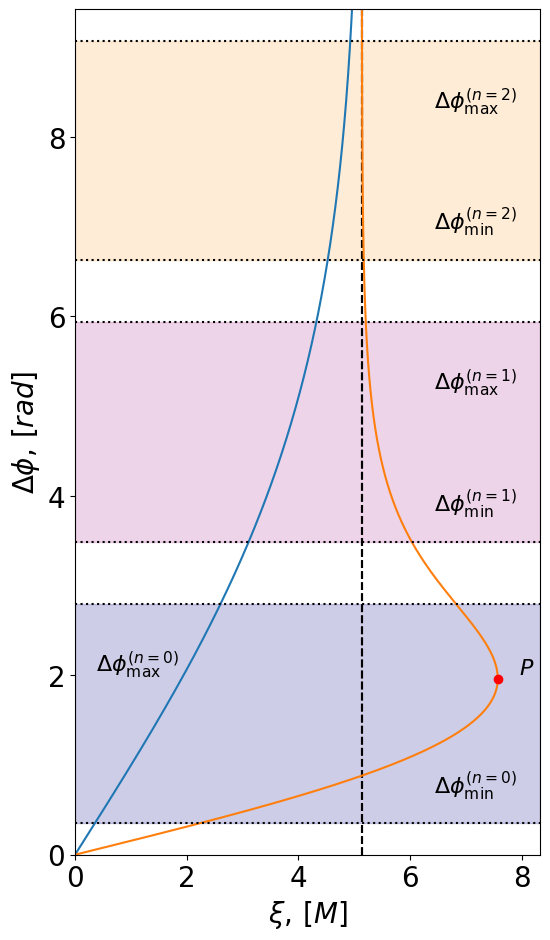
\includegraphics[scale = 0.3]{Section_6_Morphology_of_the images_of_horizonless_spacetimes/WH_70_deg_r6_impact_gamma_2.png}
			\caption{The solution to the equation (4.5) $\Delta\phi(\xi)$ for both types of trajectories.} \label{fig:1a}
		\end{subfigure}\,\,\,
		\begin{subfigure}{8cm}
			\hspace{-0.25cm}
			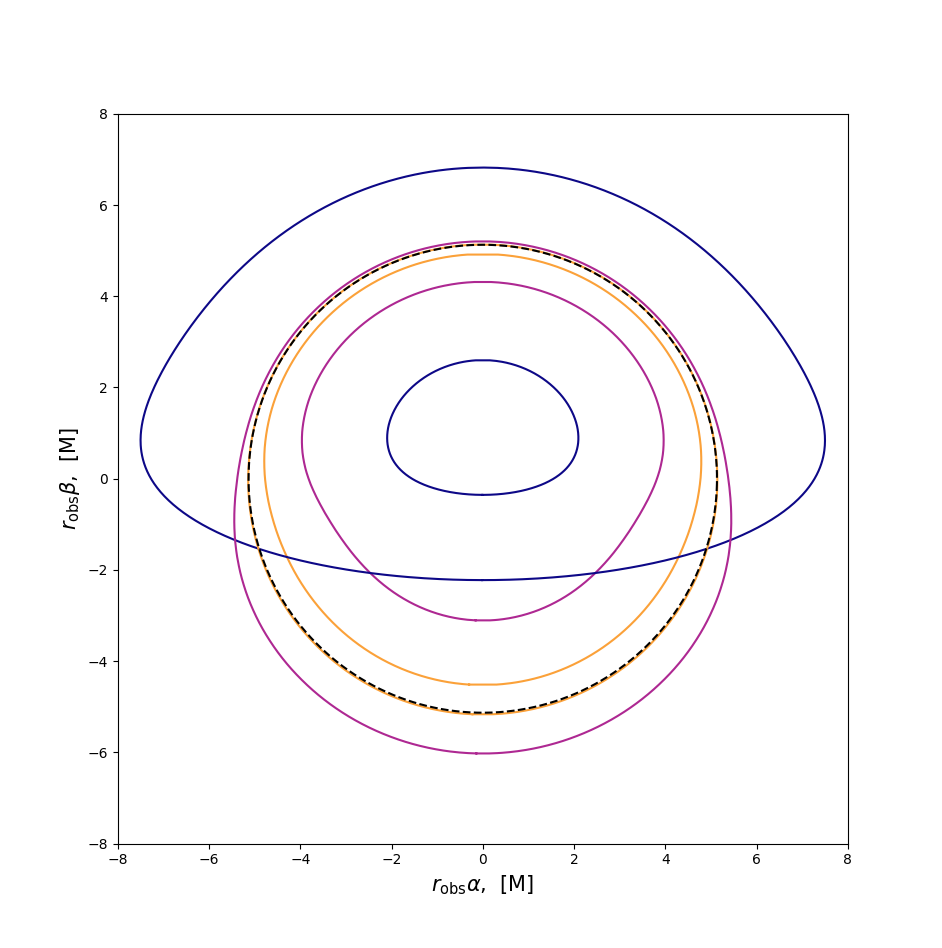
\includegraphics[scale = 0.27]{Section_6_Morphology_of_the images_of_horizonless_spacetimes/WH_70_deg_r6_gamma_2.png}
			\caption{Images constructed from $\Delta\phi(\xi)$.\newline} \label{fig:1b}
		\end{subfigure}
		\caption[$\Delta\phi(\xi)$ and the images for a $r_s=6M$ orbit around a wormhole for $n = 0,1,2$.]{\small $\Delta\phi(\xi)$ (a) and the constructed images for $n \in [0,2]$ (b) for an $r_s=6M$ around a wormhole with $\gamma = 2$ and an observer with $r_\text{obs} = 10^3M,\,\,i = 70^\circ$. The black curve corresponds to the rim of the shadow.} 
		\label{WH_r6_orbit}
	\end{figure}
	
	We can immediately notice a significant morphological difference compared to a Schwarzschild black hole. In this case there exists a class of photons with impact parameters $\xi \le \xi_\text{crit}$ (the blue curve in figure 2.1a), which form additional images \emph{inside} the shadow region. They correspond for the orbit $r_s = 6M$ on the \emph{other} side of the wormhole throat. Due to their small impact parameter, they pass under the photon sphere and "fall"$\,$onto the throat, at which point they scatter on the other side to reach the observer. The presence of of a symmetric photon sphere results in the generation of \emph{two} infinite sets of images for each value of $n$. We can also notice that the exotic images converge to the rim of the shadow significantly more slowly with increasing $n$.\\
	
	Given that the main topic of interest to us is the ability to observe these exotic images, let us examine the expected size of not just one orbit, but the \emph{whole} emission medium. On figure \ref{WH_img_size_deg} we can see the generated contours for the exotic images of orbits with $r_s = \{6M, 500M\}$ for $n\in[0,2]$ and inclinations $i = \{20^\circ,70^\circ\}$.\\
	
	\begin{figure}[!htb]
		\centering
		\begin{subfigure}{6cm}
			\hspace{-0.8cm}
			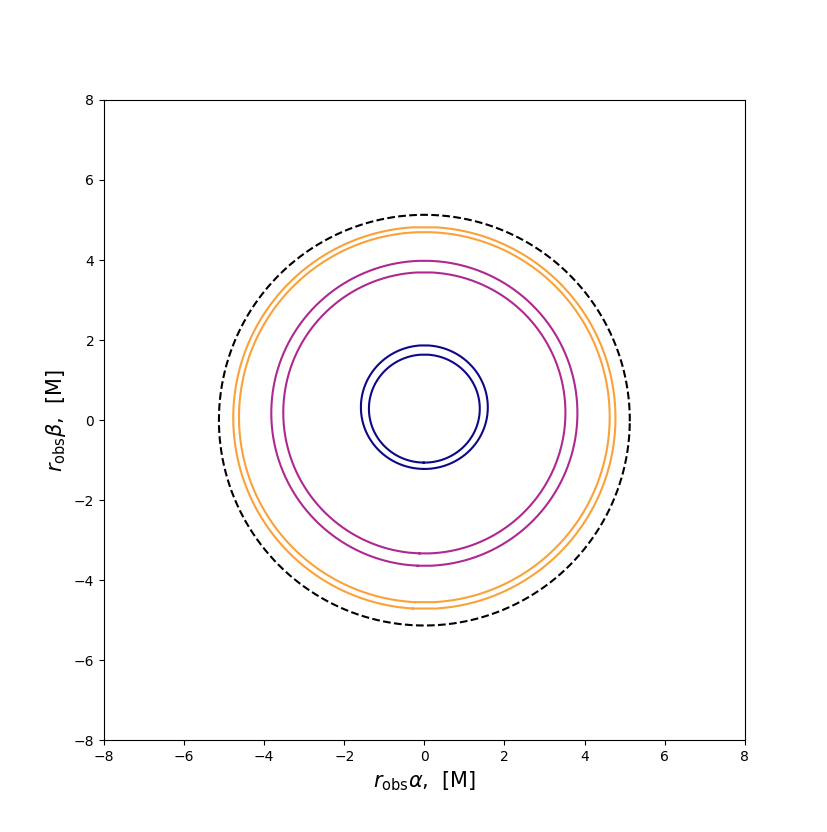
\includegraphics[scale = 0.25]{Section_6_Morphology_of_the images_of_horizonless_spacetimes/WH_20_deg_r6_r500.png}
			\caption{$r_s = \{6M, 500M\},\,\, i = 20^\circ$.}
		\end{subfigure}\,\,\,
		\begin{subfigure}{6cm}
			\hspace{-0.3cm}
			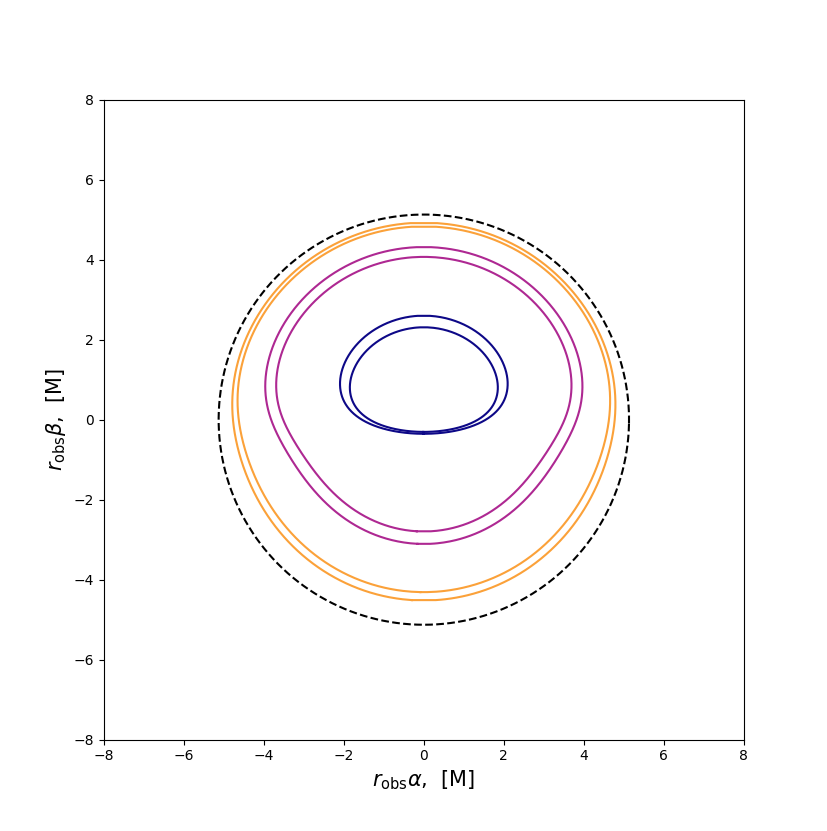
\includegraphics[scale = 0.25]{Section_6_Morphology_of_the images_of_horizonless_spacetimes/WH_70_deg_r6_r500.png}
			\caption{$r_s = \{6M, 500M\},\,\, i = 70^\circ$.}
		\end{subfigure}
		\caption[The characteristic size of the exotic images of the whole emission medium around wormholes.]{\small The characteristic size of the exotic images of the whole emission medium around wormholes. The back curve corresponds to the rim of the shadow.} 
		\label{WH_img_size_deg}
	\end{figure}
	
	We see that the direct image, which for emission from "our"$\,$ side of the throat is responsible for most of the observed flux, is concentrated in a very thin region inside the shadow. This suggests that these images can potentially be very intense and thus be extremely relevant to observations. We will now investigate this using the Novikov-Thorne model \cite{Page1973}, according to which the flux emitted from the surface of the accretion disk, and measured by an observer comoving with it $F(r)$ is given by:
	
	\begin{equation}
		F(r) = - \frac{\dot{M}}{4\pi\sqrt{-g^{(3)}}}\frac{\partial_r\Omega}{\left(E - \Omega L_z\right)^2}\int_{r_\text{ISCO}}^r \left(E - \Omega L_z\right)\partial_rL_zdr^\prime,
	\end{equation}
	where $E = E(r)$, $L_z = L_z(r)$ and $\Omega = \Omega(r)$ are the time averaged energy, angular momentum and angular velocity of the emitting medium (given by the expressions (D.12), (D.15a) and (D.15b) of the dissertation) and $g^{(3)}$ is the determinant of the induced in the equator metric. This flux needs to be corrected to account for the relative motion between the emission medium and the observer:
	
	\begin{equation}
		F(r)\rightarrow\mathcal{F}(r,\phi) = \left(\frac{1}{1+z} \right)^4 F(r),\quad \frac{1}{1 + z} = \frac{k_\mu v^\mu\vert_{\vec{r} = \vec{r}_\text{obs}}}{k_\nu u^\nu\vert_{\vec{r} = \vec{r}_\text{emitter}}},
	\end{equation}
	where $v^\mu$ is the velocity of the observer, $u^\mu$ is the average velocity of the emission medium and $k^\mu$ is the photon momentum. Let us now simulate observations of the object M87$^*$ by fixing the mass in the metric to $M = 6.2\times10^9 M_\odot$ and the distance to the object to $r_\text{obs} = 16.4 \text{Mpc}$. On figure \ref{WH_NT} we show such a disk around a wormhole with $\gamma = 2$ at two different inclination angles $i=\{20^\circ, 70^\circ\}$. On the right panels we show the horizontal slices $\delta_\text{rel} = 0$. The colormap is normalized to the maximum of each image.
	
	\newpage
	
	\begin{figure}[!htb]
		\centering
		\begin{subfigure}{12cm}
			\hspace{-0.6cm}
			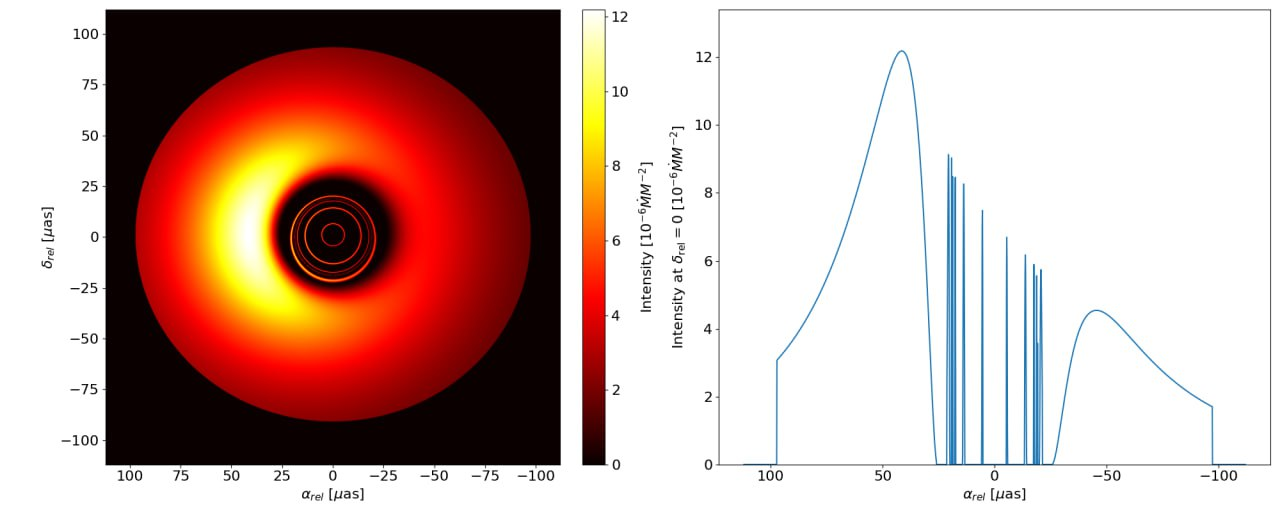
\includegraphics[scale = 0.4]{Section_6_Morphology_of_the images_of_horizonless_spacetimes/WH_NT_Gamma2_20_deg.jpg}
			\caption{$i = 20^\circ$} 
		\end{subfigure}
		\begin{subfigure}{12cm}
			\hspace{-0.6cm}
			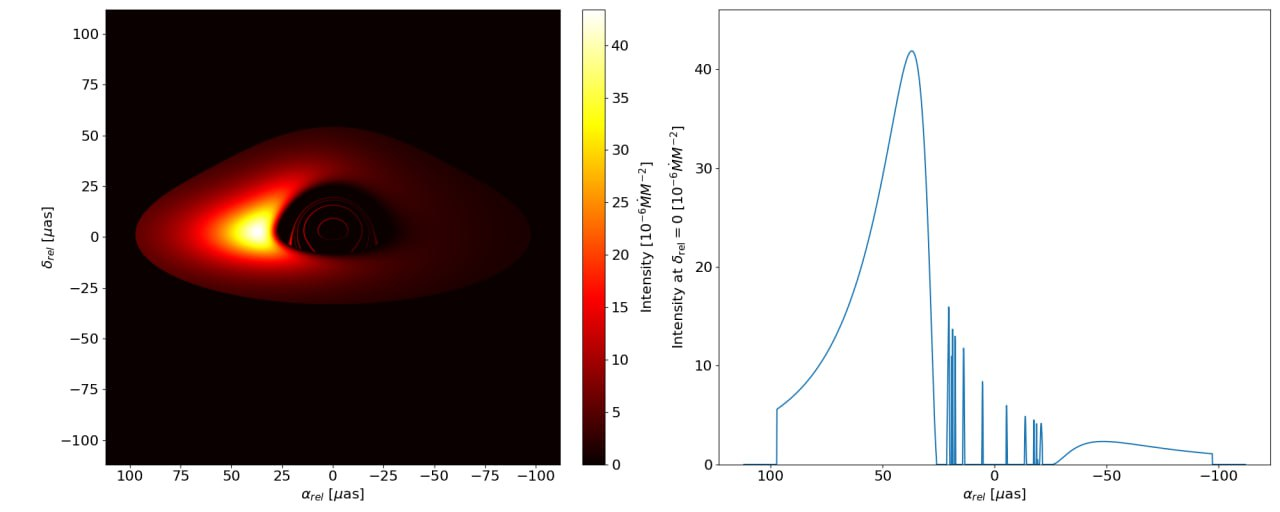
\includegraphics[scale = 0.4]{Section_6_Morphology_of_the images_of_horizonless_spacetimes/WH_NT_Gamma2_70_deg.jpg}
			\caption{$i = 70^\circ$} 
		\end{subfigure}
		\caption[A Novikov-Thorne disk around a wormhole at different inclinations.]{\small A Novikov-Thorne disk around a wormhole with $\gamma = 2$ at different inclinations. The disk parameters are $r_\text{in} = r_\text{ISCO}$ and $r_\text{out} = 25M$.} 
		\label{WH_NT}
	\end{figure}
	
	We see that at low inclinations the central exotic images have an intensity that is comparable to the maximum of the whole image, while at low inclination the strong Doppler effect of the disk region that is moving towards the observer dominates, and the central images are suppressed by approximately one order of magnitude. Based on this we can conclude the following:\\
	
	\emph{For low inclinations the exotic images of wormholes are \emph{highly} observationally relevant, while at low inclinations their detection is comparably more difficult, but not unreasonable.}
	
	\newpage
	
	\section{The spacetime imprint on the polarization of the images of exotic compact objects}
	
	In this chapter we will summarize the results from publications II and II, as well as chapter \emph{6} of the dissertation. We study how the nature of the ambient spacetime around supermassive compact objects affects the polarization of the observed emission. In chapter \emph{3} of the dissertation we presented the current results of the EHT collaboration for the supermassive objects M87$^*$ and Sgr A$*$. Similar future studies will increase the resolution and expand the set of observed object but the main challenges in interpreting the result will still remain. They are the following:\\
	
	\textbf{1)} \emph{The unambiguous determination the nature of the compact object, along with the gravitational theory that describes it.}\\
	
	\textbf{2)} \emph{Determining the physical state of the emission medium.}\\
	
	Answering the above two questions simultaneously is a highly non-trivial question. On one side the nature of the spacetime  around the compact object is non-linearly coupled to the magnetohydrodynamics of the emission medium, which makes studying just one of the above questions impossible. On the other side, the morphology of the observed images (even though it contains information about the spacetime) is highly degenerate between spacetimes with a drastically different physical nature. Moreover, it is possible that different spacetimes posses mathematically \emph{identical} shadows \cite{PhysRevD.103.084040}, which means that one \emph{cannot} fix the nature of the spacetime, based only on the morphology of the observed images. We therefore need additional sources of information, characterizing the immediate vicinity around these objects.\\
	
	One such source is the polarization of the observed radiation. It characterizes the structure of the magnetic field in the emission region and, even more importantly for us, its propagation to the observer is influenced by the geometry of the ambient spacetime. As the analysis performed by the EHT collaboration shows, this additional source of information can lift (but not entirely) the degeneracy of the problem of interpreting the images. Motivated by this, we use a simplified analytical model, described in \cite{Narayan2021}, and generalized to arbitrary static and spherically symmetric spacetimes in publication II (chapter \emph{6} of the dissertation) to study the imprint of the stapcetime on the polarized images.
	\newpage
	
	More concretely our goals are:\\
	
	\textbf{1)} \emph{To determine weather the polarized images of the emission medium around exotic compact objects posses qualitatively different features, based on which we can distinguish them from Scwarzshild black holes. Our working hypothesis is that the observed images will be qualitatively similar to those of M87$^*$.}\\
	
	\textbf{2)} \emph{To give a quantitative estimate for the influence of the spacetime on the polarized images.}\\
	
	We will focus our studies on static, spherically symmetric wormhole spacetimes and the Janis-Newman-Winicour naked singularity. Similar studies have been conducted for rotating Kerr black holes in \cite{Gelles2021}, and for certain objects in modified theories of gravity in \cite{Qin2021}. Some general theoretical properties of the polarized emission around Kerr black holes have been studied in \cite{Himwich2020}, based on the classical works  \cite{Luminet1979}, \cite{Connors1980}, \cite{Chen1991}.\\
	
	To give the reader a better context on the results of the author, presented in section 3.2, we will first go over the analytical model of the emission medium.
	
	\subsection{Analytic model of the emission medium}
	
	The more in-depth discussion of this model can be found in chapter \emph{6} of the dissertation. Here we will only give the main aspects of the model.\\
	
	We consider an emitting fluid, moving on a circular orbit around a compact object, described by a general static and spherically symmetric metric of the form:
	
	\begin{equation}
		ds^2 = - e^{2\nu(r)}dt^2 + e^{2\lambda(r)}dr^2 + R^2(r)\left(d\theta^2 + \sin^2\theta d\phi^2\right).
	\end{equation}
	
	\noindent We parameterize the fluid velocity $\vec{\beta}$ using its magnitude $\beta$ and orientation angle $\chi$:
	
	\begin{equation}
		\vec{\beta} = \beta\left[\cos\chi (r) + \sin\chi (\phi)\right].
	\end{equation}
	
	After that we introduce, in the local basis of this fluid, the magnetic field $\vec{B} = (\hat{B}^{(r)},\hat{B}^{(\phi)},\hat{B}^{(\theta)})$ and the local three-dimensional photon momentum $\vec{p} = \left(\hat{p}^{(r)},\hat{p}^{(\phi)},\hat{p}^{(\theta)}\right)$. Under the action of the magnetic field, the fluid emits synchotron radiation with a polarization vector $\vec{f}$, which is given in the fluid frame as:
	\begin{equation}
		\vec{f} = \frac{\vec{p}\times\vec{B}}{|\vec{p}|},
	\end{equation}
	where we will use the gauge freedom to enforce the condition $\hat{f}^{(t)} = 0$. Then the magnitude of the polarization vector satisfies the following condition:
	\begin{equation}
		\hat{f}^{(a)}\hat{f}_{(a)} = \sin^2\zeta|\vec{B}|^2,
	\end{equation}
	
	Where we have labeled with $\zeta$ the angle between $\vec{p}$ and the magnetic field $\vec{B}$. From here the our task is to calculate how the vector $\vec{f}$, defined by (3.3), is transported to a distant observer. In the general case this would be done by solving the equation of parallel transport $p^\mu\nabla_\nu f^\nu = 0$, but we can use the symmetries of the spacetime, described by (3.1) to algebrize the problem. More-concretely we can use the existence of a Killing-Yano tensor $Y_{\mu\nu}$ with the following non-zero components:
	
	\begin{equation}
		Y_{\theta\phi} = -Y_{\phi\theta} = R^3(r)\sin\theta,
	\end{equation}
	
	\noindent to form the following integrals of motion\footnote{With the help of a Lorentz transformation, using the velocity $\vec{\beta}$ (3.2), the expressions for $\kappa_1$ and $\kappa_2$ can be expressed entirely through the initial conditions $\vec{f}$ and $\vec{p}$ in the reference frame of the fluid. For more details we refer the reader to section 6.1 of the dissertation.}:
	
	\begin{subequations}
		\begin{equation}
			\kappa_1 = \frac{1}{4}\epsilon_{\mu\nu\alpha\beta}Y^{\alpha\beta}p^\mu f^\nu
		\end{equation}
		\begin{equation}
			\kappa_2 = Y_{\mu\nu}p^\mu f^\nu
		\end{equation}
	\end{subequations}
	
	With their help one can show that the measured by a distant observer polarization vector $\vec{f}_\text{obs}$, projected onto the observation plane, has the following form:
	
	\begin{subequations}
		\begin{equation}
			f^x_\text{obs} = \frac{x\kappa_1 + y\kappa_2}{\sqrt{(x^2 + y^2)(\kappa_1^2 + \kappa_2^2)}}
		\end{equation}
		\begin{equation}
			f^y_\text{obs} = \frac{y \kappa_1 - x\kappa_2}{\sqrt{(x^2 + y^2)(\kappa_1^2 + \kappa_2^2)}},
		\end{equation}
	\end{subequations}
	
	where $x$ and $y$ are the Cartesian coordinates on the image, given by the expressions:
	
	\begin{subequations}
		\begin{equation}
			x = -R(r)p^{(\phi)} = -\frac{p_\phi}{\sin\theta_\text{obs}}
		\end{equation}
		\begin{equation}
			y = R(r)p^{(\theta)} = p_\theta
		\end{equation}
	\end{subequations}
	
	As a last step, let us form the two observational quantities: the polarized intensity $I$ and the rotation angle of the electric field vector $EVPA$. The second one is defined trough the expressions (3.7) as:
	
	\begin{equation}
		EVPA = \arctan\left(-\frac{f^x_\text{obs}}{f^y_\text{obs}}\right),
	\end{equation}
	
	\noindent while to define the intensity we need to take into account certain phenomenological effects of the emission process. First, it depends on the angle between the emission direction (photon momentum) and the magnetic field vector as $I\propto \left(\sin\chi\right)^{1+\alpha_\nu}$. Second, any realistic physical medium is not purely equatorial and the emission mechanism is defined per unit volume. The intensity then needs to be further corrected by the length of the geodesic inside the emission medium $\ell_p$. For an optically and geometrically thin accretion disk this length is given by:
	
	\begin{equation}
		\ell_p = \bigg\vert\frac{\hat{p}^{(t)}}{\hat{p}^{(\theta)}}\bigg\vert H.
	\end{equation}
	
	\noindent Lastly we need to account for the relativistic Doppler effect. We do this with an additional multiplicative factor of $g^{3 + \alpha_nu}$, where $g$ is defined as:
	
	\begin{equation}
		g = \frac{E_\text{obs}}{E_s} = \frac{1}{\hat{p}^{(t)}}.
	\end{equation}
	
	\noindent With this we can write the intensity (up to a multiplicative constant) as:
	
	\begin{equation}
		I = g^{3 + \alpha_\nu}\ell_p(\sin\zeta)^{1 + \alpha_\nu}.
	\end{equation}
	
	\noindent The models for $M87^*$ are consistent with a value $\alpha_\nu = 1$, which we will use for our studies.\\
	
	We thus reduce the problem to choosing an initial condition for the polarization vector in the rest frame of the fluid (3.3) and then evaluating $\vec{f}_\text{obs}$ with the help of (3.6) and (3.7). This choice of an initial condition requires fixing a number of free model parameters. They are:\\
	
	\textbf{1)} The velocity vector $\vec{\beta}$ and the magnetic field profile $\vec{B}$ in the fluid rest frame. We choose these parameters following previous studies of this topic for Scwarzchild black holes \cite{Narayan2021}. The authors there propose values which best describe the observed structure of the polarization of the M87$^*$.\\
	
	\textbf{2)} The photon momentum $\vec{p}$ at the point of emission, measured in the rest frame of the fluid. For the case of Schwarzschild black holes, the authors in \cite{Narayan2021} use an analytical approximation for the equations of motion for null geodesics to calculate the momenta in (3.3) analytically. Unlike them we use the numerical code developed by the author Mjølnir\footnote{The code itself can be found at https://github.com/ValentinDeliyski/Mjolnir\_GRRT. In appendix B of the dissertation the reader can find a description of its functionality, along with a comparison with similar codes, based on the publication \cite{Gold2020}} for their calculation.
	\newpage
	\subsection{Results}
	
	We start our study from the first main result of the authors in \cite{Narayan2021} - the fact that vertical magnetic fields cannot reproduce the observed morphology of the polarized images of M87$^*$, assuming that the object is a Schwarzschild back hole. We want to determine to what extent this result depends on the nature of the underlying spacetime. On figure 3.1 we show our results for the wormhole spacetime, described by the line element (2.1) (panel a and b) and for the Janis-Newman-Winicour naked singularity (panels c and d). The colormap corresponds to the one free parameter in the corresponding metrics, labeled $\gamma$.\\
	
	We see that up to a displacement of the visible position of the images, the general morphology remains unchanged. Both class exotic compact object generate polarized images which do not exhibit the characteristic for M87$^*$ twist of the polarization vector. Furthermore the apparent position of the maximum remains in the lower part of the image, which is inconsistent with observations (where this maximum is located on the right side of the image). We can therefore conclude that vertical magnetic fields are not compatible with the observations of M87$^*$, even considering exotic compact objects. Because of this we will focus our attention only on equatorial magnetic fields.\\

	This also shows us that the polarization of the direct images is weakly sensitive to the nature of the underlying spacetime. For this reason we choose to perform a quantitative analysis of the deviations in intensity and twist of the polarization vector from the Schwarzschild black hole. Because our goal is to determine weather we can observationally distinguish exotic compact object from Schwarzschild black holes, we compare the polarization at fixed points on the observation plane $\{x,y\}$, instead of at fixed emission radii $r_s$. Due to the different level of focusing of the light rays in the spacetimes we consider, the emission radius $r_s$ in this case will vary along the image.\\
	
	
	\begin{figure}[!htb]
		\begin{subfigure}{7cm}
			\hspace{0.0em}
			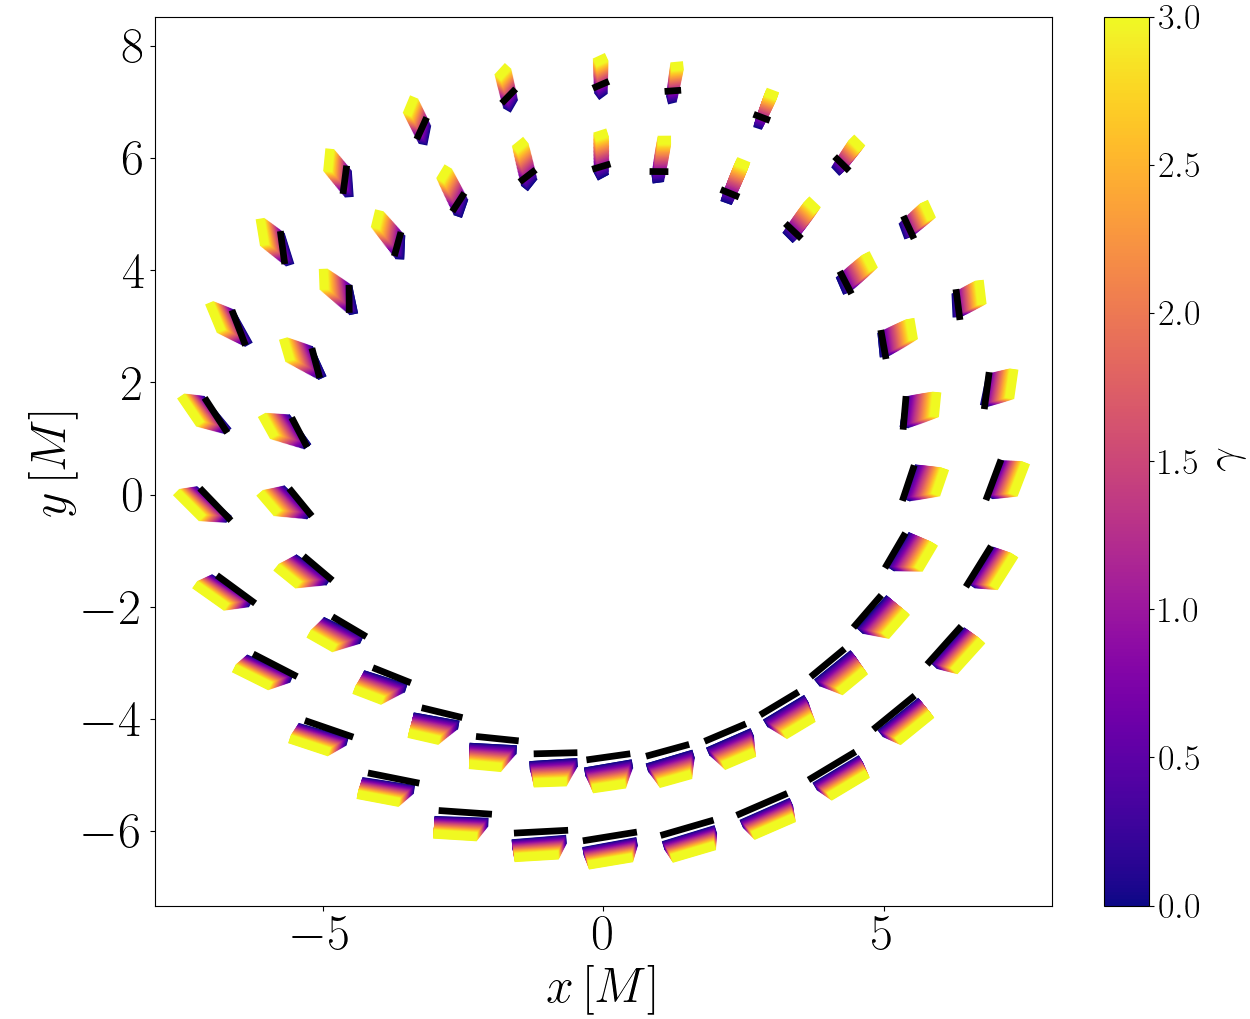
\includegraphics[scale = 0.23]{Section_7_Polarized_Emission/WH_alpha_Vert_Field.png}
			\caption{Wormhole, \\$\beta = 0.3$, $\chi = -150^\circ$.} 
		\end{subfigure}\,\,\,
		\begin{subfigure}{7cm}
			\hspace{0.2em}
			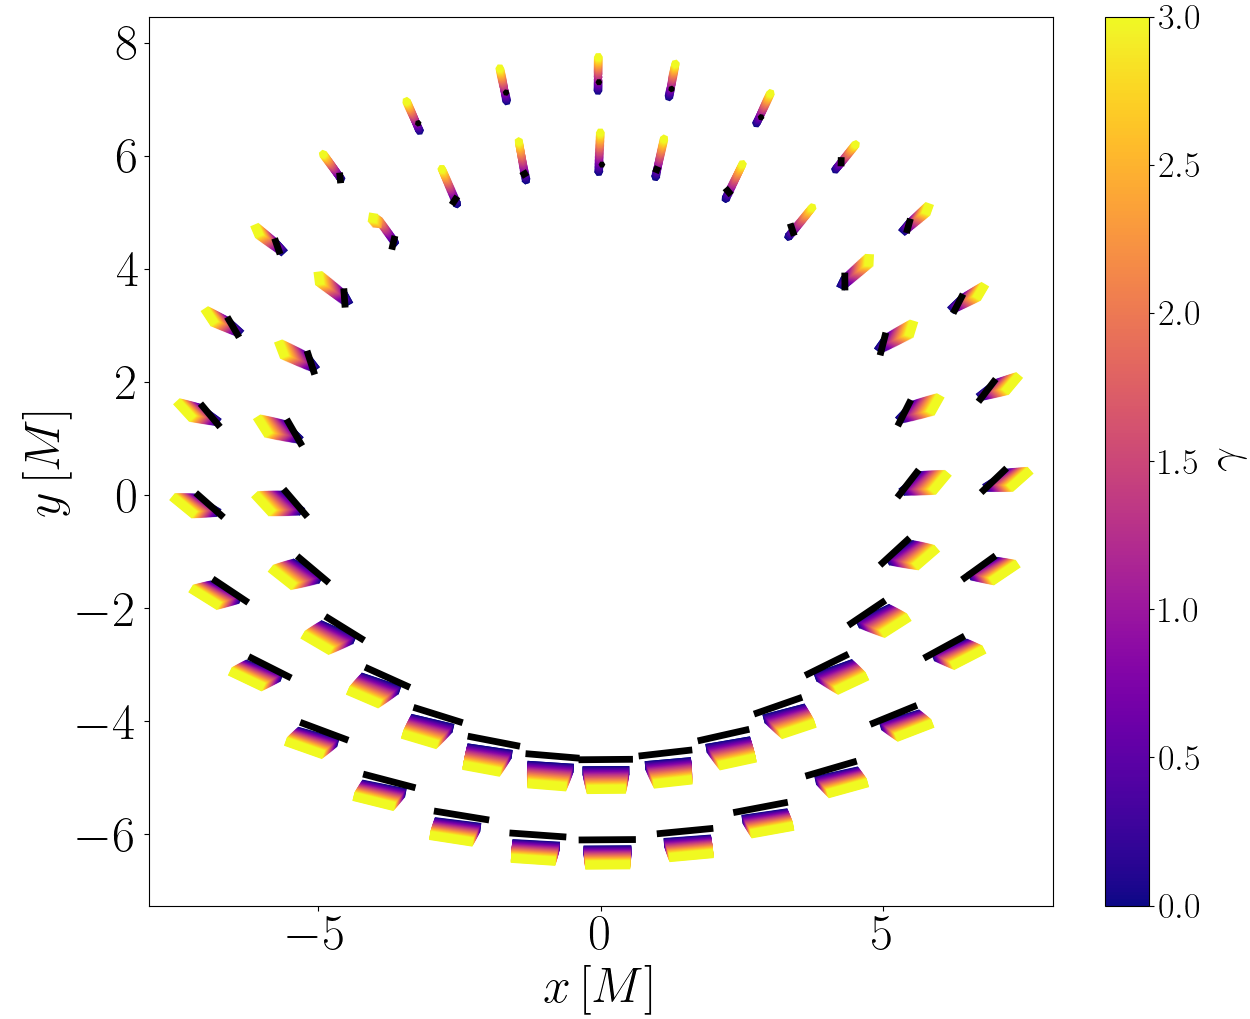
\includegraphics[scale = 0.23]{Section_7_Polarized_Emission/WH_alpha_Vert_Field_beta_zero.png}
			\caption{Wormhole, \\$\beta = 0$, $\chi = -150^\circ$.}
		\end{subfigure}\\
		\begin{subfigure}{7cm}
			\hspace{0.0em}
			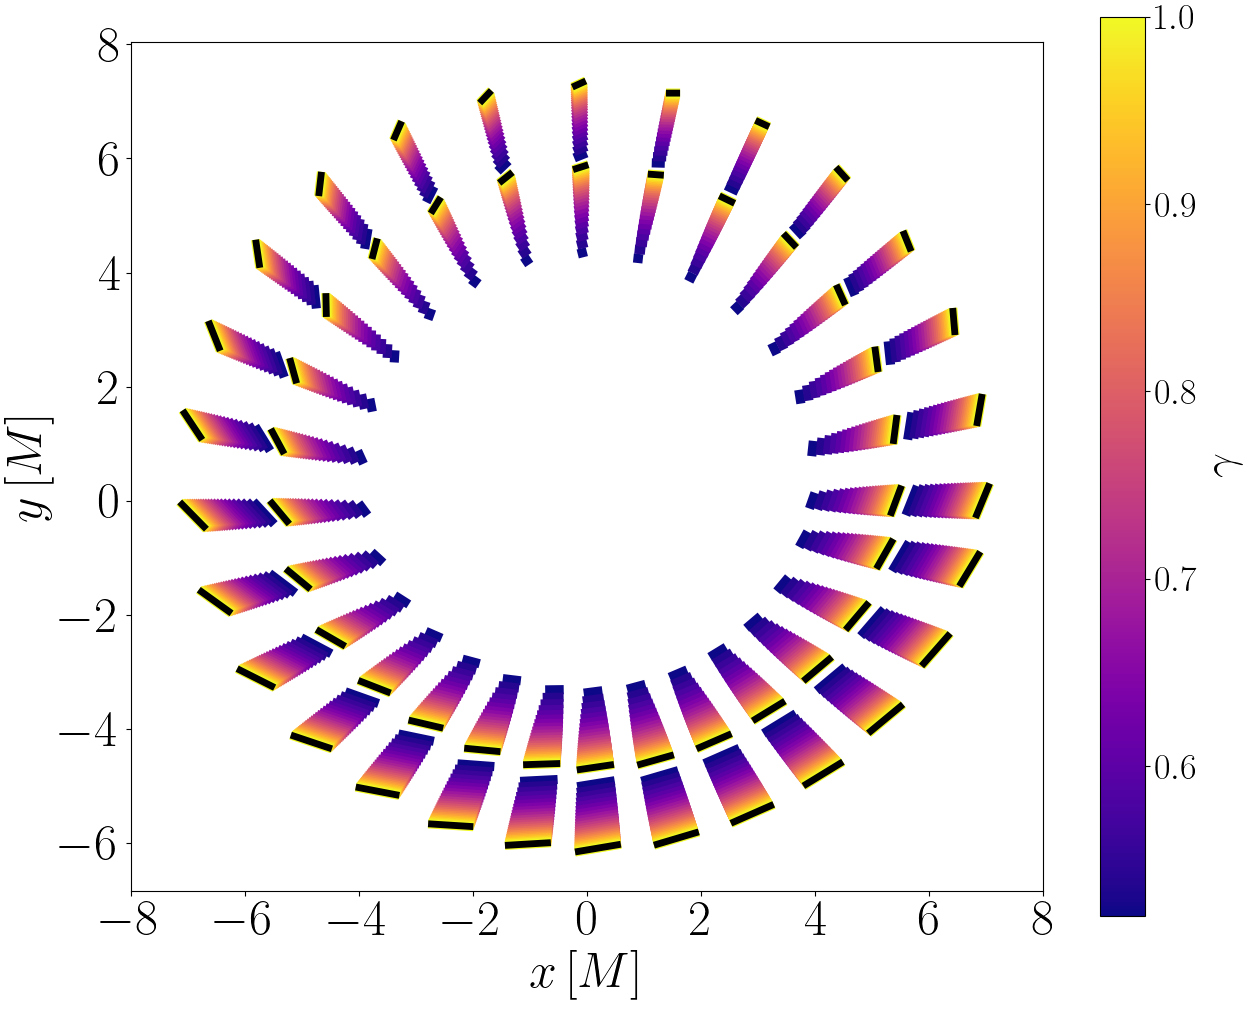
\includegraphics[scale = 0.23]{Section_7_Polarized_Emission/JNW_alpha_Vert_Field.png}
			\caption{Janis-Newman-Winicour naked singularity, $\beta = 0.3$, $\chi = -150^\circ$.} 
		\end{subfigure}\,\,\,
		\begin{subfigure}{7cm}
			\hspace{0.2em}
			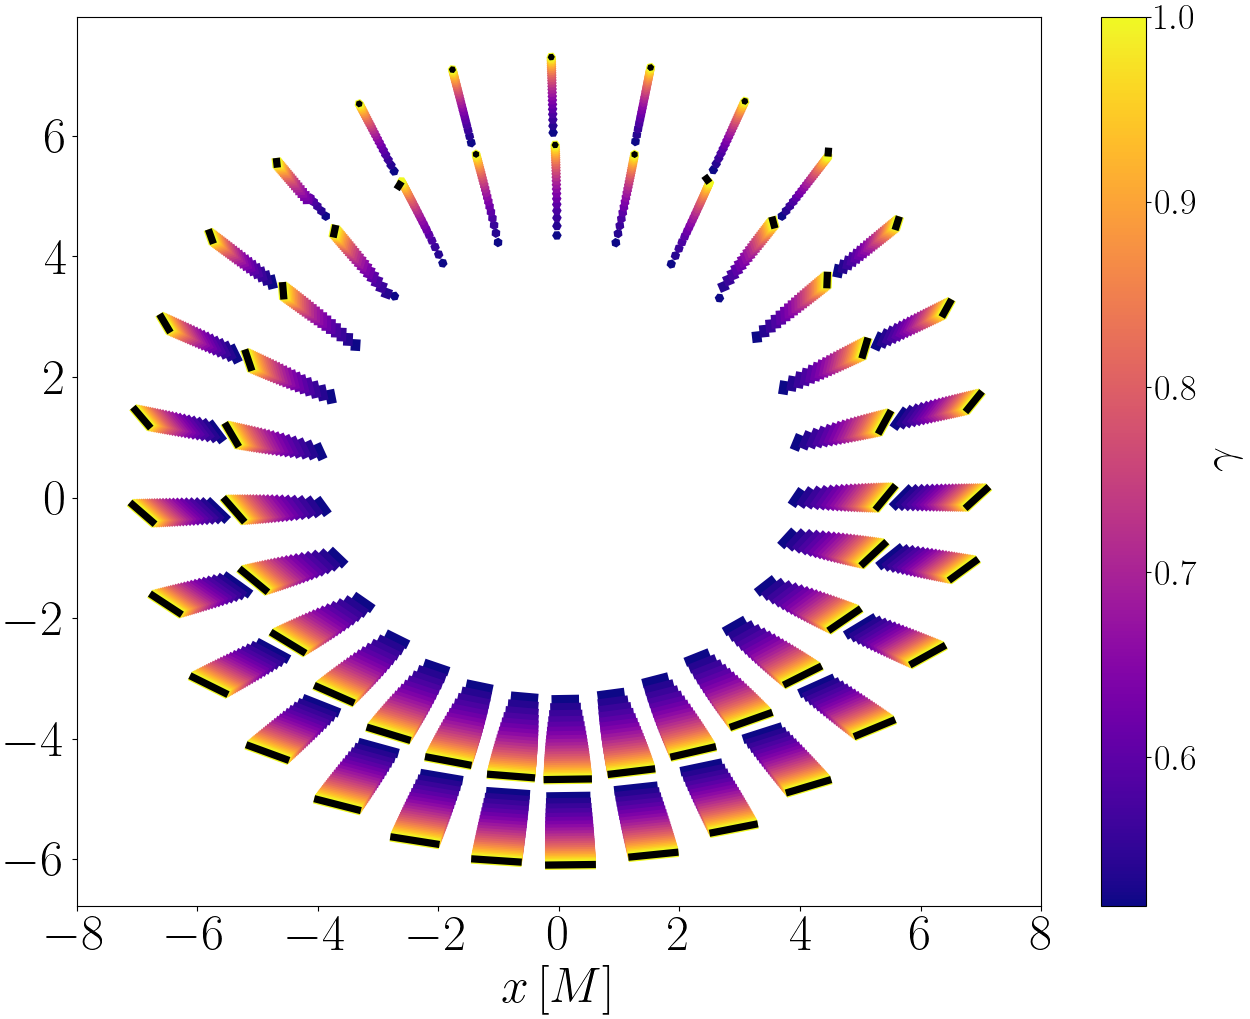
\includegraphics[scale = 0.23]{Section_7_Polarized_Emission/JNW_alpha_Vert_Field_beta_zero.png}
			\caption{Janis-Newman-Winicour naked singularity, $\beta = 0$, $\chi = -150^\circ$.}
		\end{subfigure}
		\caption[The direct polarized images around wormholes and naked singularities for a vertical magnetic field.]{\small
			The constructed direct polarized images of the orbits $r_s = 6M$ and $r_s = 4.5M$ around wormholes and naked singularities for an inclination  $i = 20^\circ$. The black lines represent a Schwarzschild black hole.} 
		\label{pol_vert_field}
	\end{figure}
	
	On figures 3.2 and 3.3 we show our analysis of polarized images, located at coordinates $\{x,y\}$, corresponding to the apparent position of the  $r_s = 6M$ orbit around a Schwarzschild black hole (we will label these in the text as $\{x,y\}\vert_{6M, \text{Schw}}$). For each image we plot the intensity $I$ and position angle $EVPA$ as a function of the azimuthal coordinate $\phi = \arctan(y / x)$. Additionally we plot the deviations from the Schwarzschild black hole $\Delta I = I_{\text{WH}} - I_{\text{Schw}}$ and $\Delta EVPA = EVPA_\text{WH} - EVPA_\text{Schw}$ for each point on the images. We show the case for a magnetic field of the form $\vec{B} = [0.87, 0, 0.5]$\footnote{The reader can find a more extended analysis with two more magnetic field configurations in section \emph{6} of the dissertation} (suggested by \cite{Narayan2021} as best describing $M87^*$) and inclinations $i = \{20^\circ, 70^\circ\}$.
	
	\newpage
	
	\begin{figure}[!htb]
		\begin{subfigure}{16cm}
			\hspace{-1.0em}
			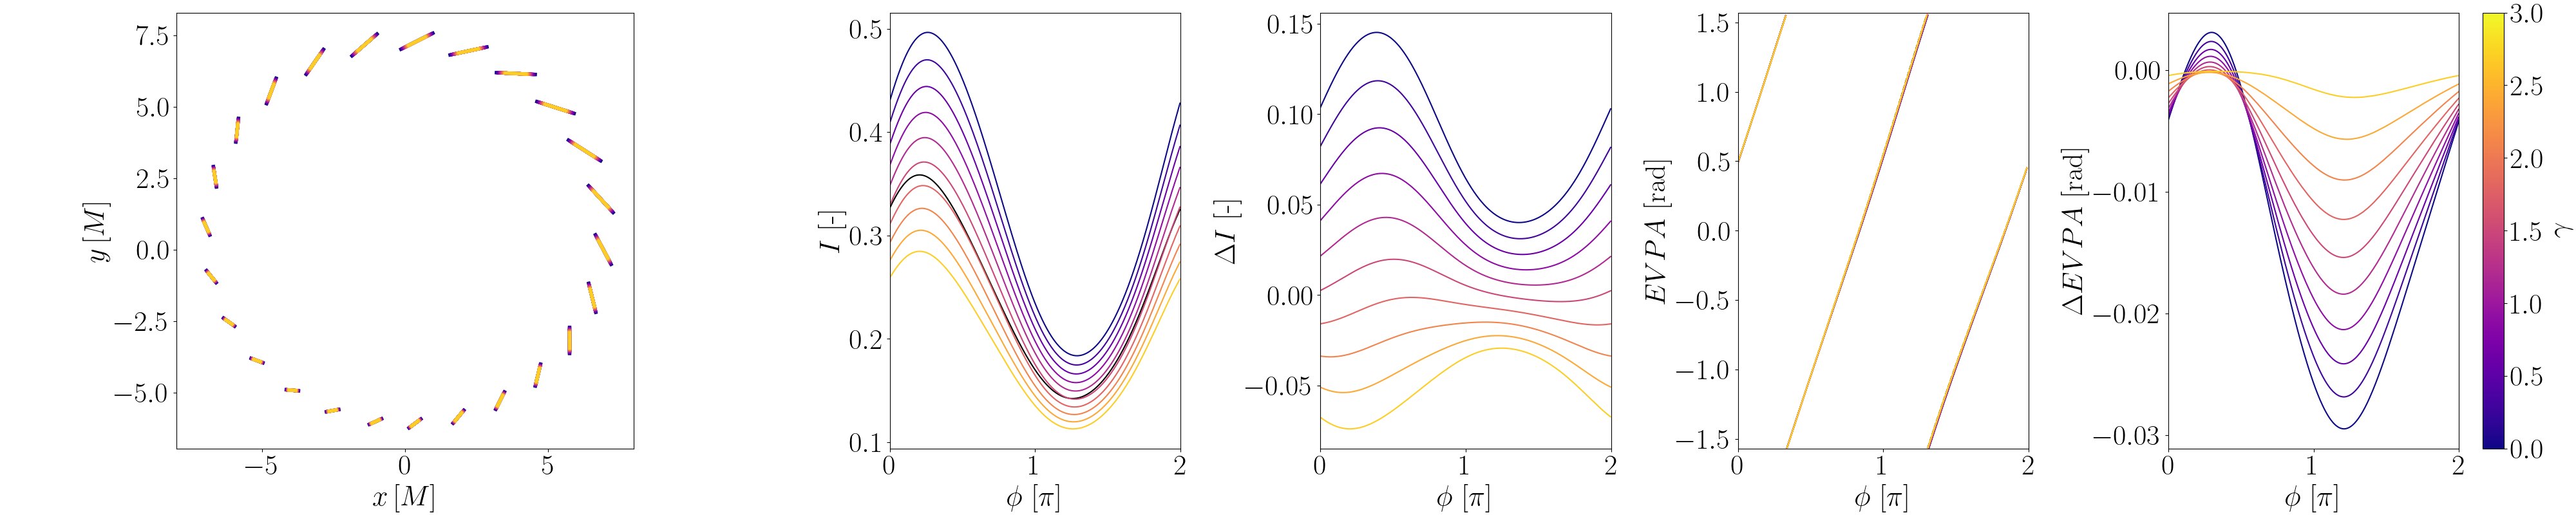
\includegraphics[scale = 0.15]{Section_7_Polarized_Emission/WH_delta_fig_B_0.87_0.5_0_20_deg_r6.png}
			\caption{Wormhole,\\ $\vec{B} = [0.87, 0, 0.5]$, $\beta = 0.3$, $\chi = -150^\circ$, $i = 20^\circ$.} 
		\end{subfigure}\\
		\begin{subfigure}{17cm}
			\hspace{-0.2em}
			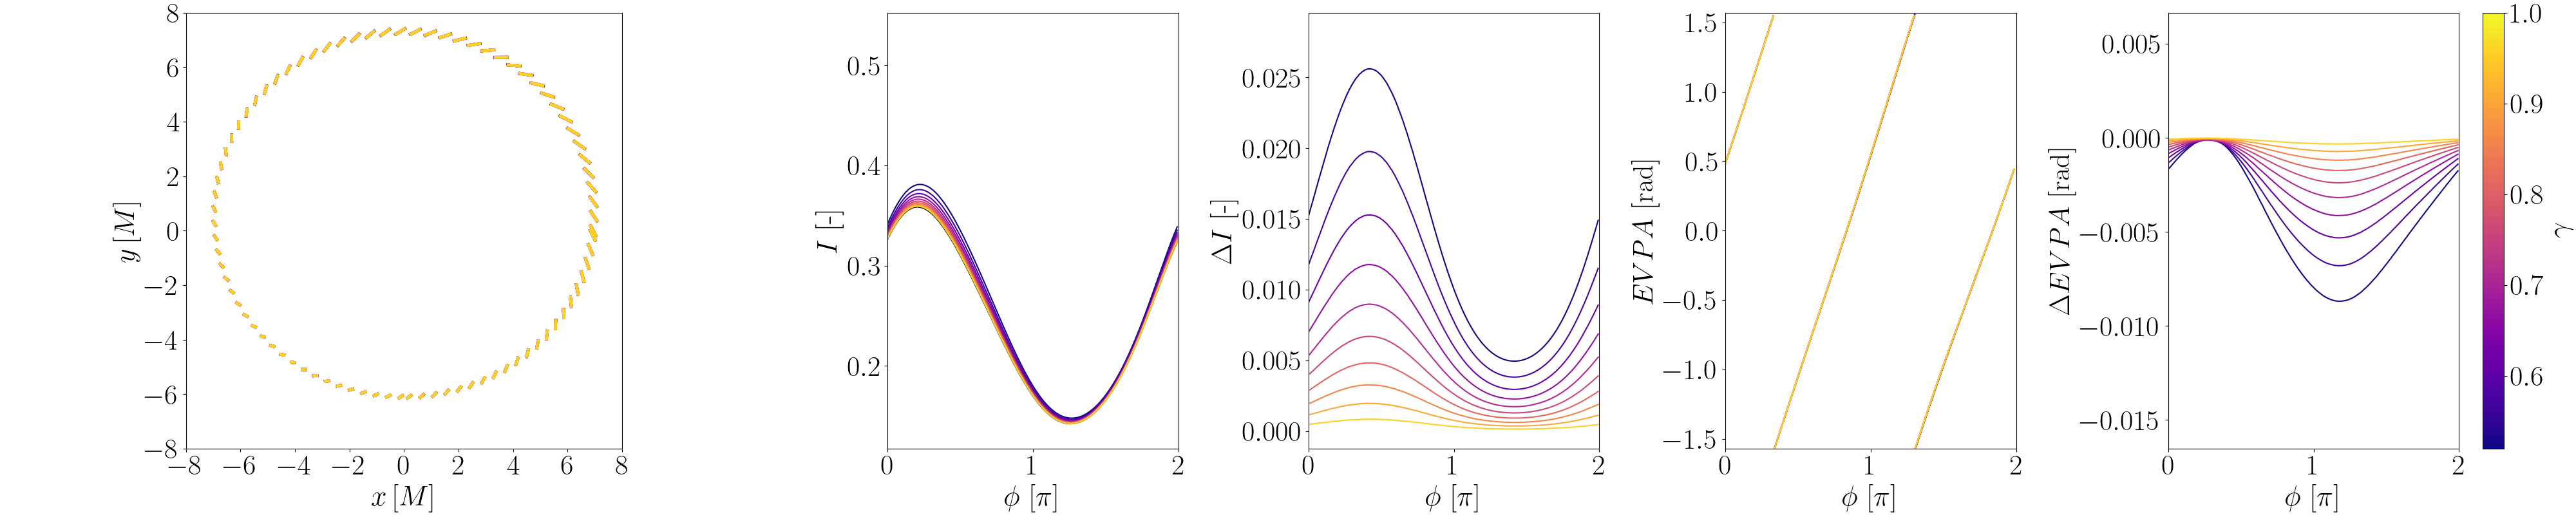
\includegraphics[scale = 0.15]{Section_7_Polarized_Emission/JNW_delta_figs_B_0.87_0.0_0.5_20_deg_direct.png}
			\caption{Janis-Newman-Winicour naked singularity,\\  $\vec{B} = [0.87, 0, 0.5]$, $\beta = 0.3$, $\chi = -150^\circ$, $i = 20^\circ$.}
		\end{subfigure}
		\caption[The polarized direct images around wormholes and naked singularities for an equatorial magnetic field at $i = 20^\circ$.]{\small The constructed direct polarized images of type $\{x,y\}\vert_{6M, \text{Schw}}$ around wormholes and naked singularities for an equatorial magnetic field and observer inclination $i = 20^\circ$. The black curves correspond to a Schwarazschild black hole.} 
		\label{Direct_image_deltas_20}
	\end{figure}
	
	
	\begin{figure}[!htb]
		\begin{subfigure}{16cm}
			\hspace{-1.0em}
			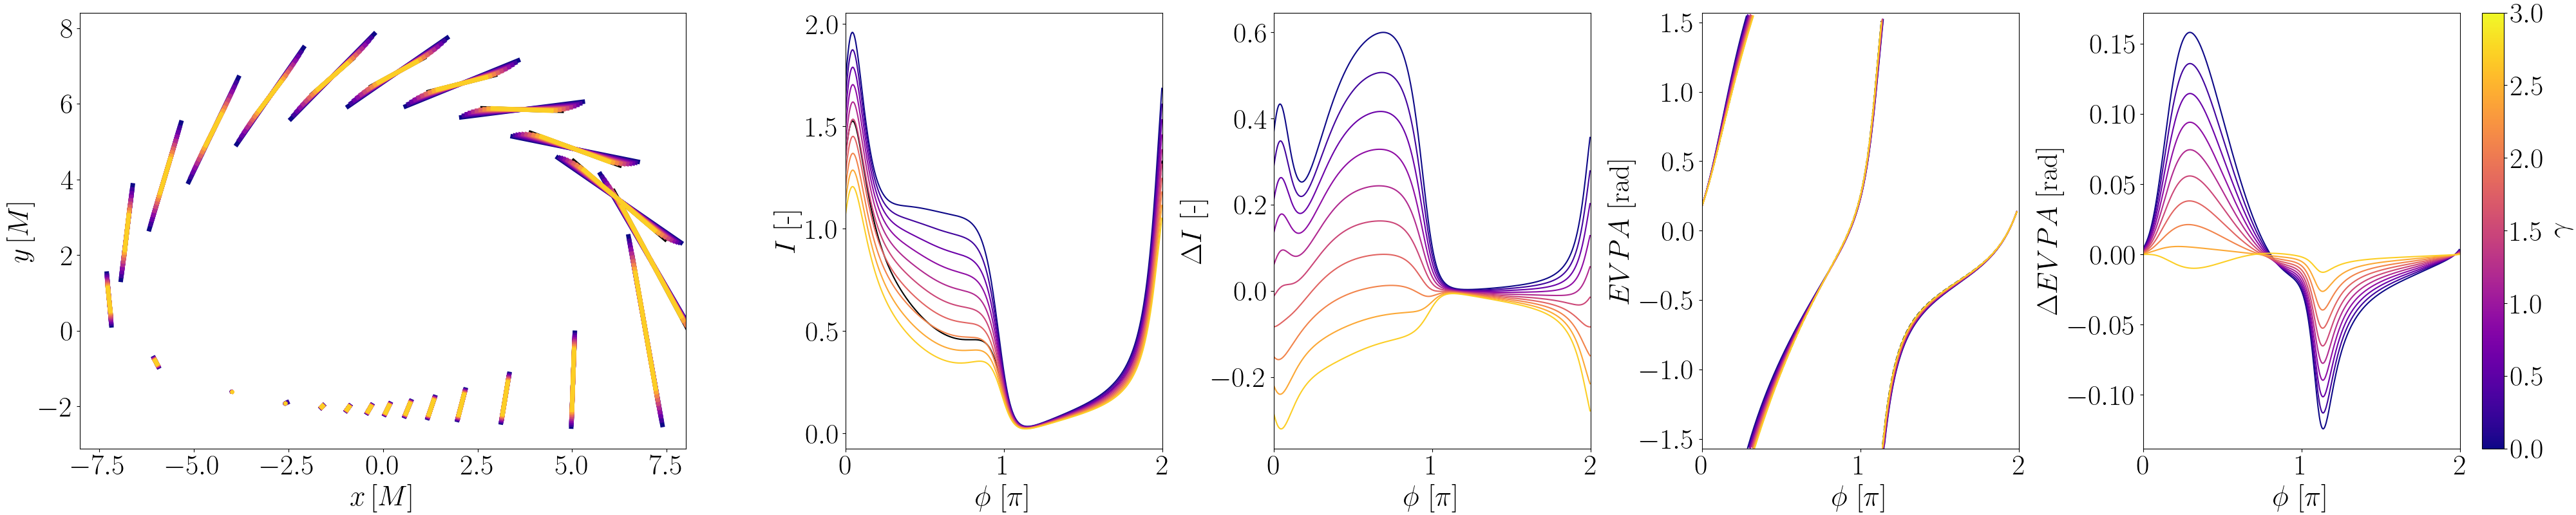
\includegraphics[scale = 0.15]{Section_7_Polarized_Emission/WH_delta_fig_B_0.87_0.5_0_70_deg_r6.png}
			\caption{Wormhole,\\ $\vec{B} = [0.87, 0, 0.5]$, $\beta = 0.3$, $\chi = -150^\circ$, $i = 70^\circ$.} 
		\end{subfigure}\\
		\begin{subfigure}{17cm}
			\hspace{-1em}
			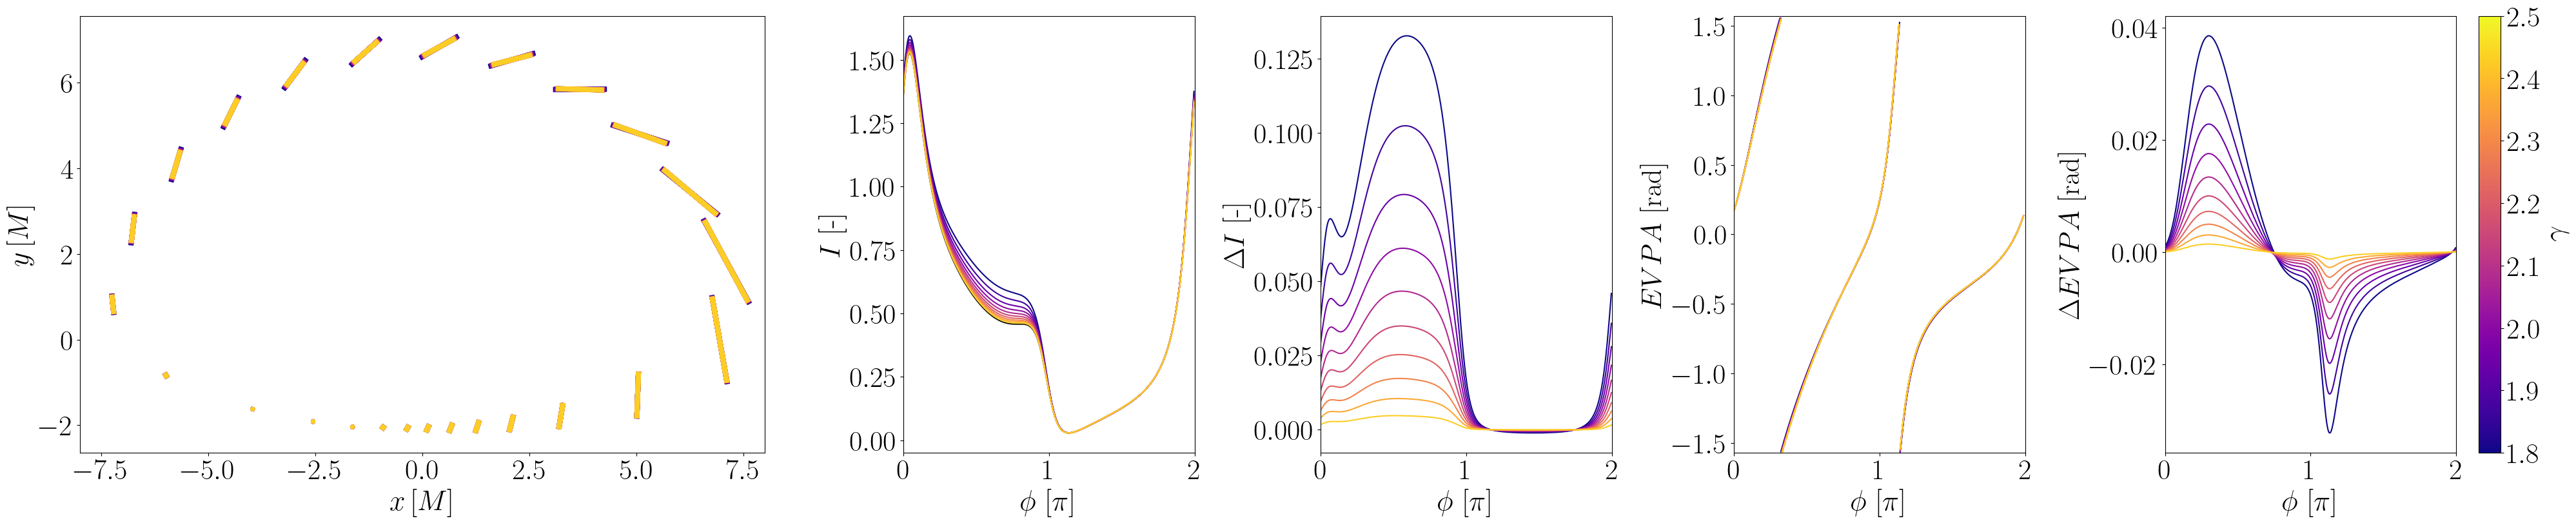
\includegraphics[scale = 0.15]{Section_7_Polarized_Emission/JNW_delta_figs_B_0.87_0.0_0.5_70_deg_direct.png}
			\caption{Janis-Newman-Winicour naked singularity,\\  $\vec{B} = [0.87, 0, 0.5]$, $\beta = 0.3$, $\chi = -150^\circ$, $i = 70^\circ$.}
		\end{subfigure}
		\caption[The polarized direct images around wormholes and naked singularities for an equatorial magnetic field at $i = 70^\circ$.]{\small The constructed direct polarized images of type $\{x,y\}\vert_{6M, \text{Schw}}$ around wormholes and naked singularities for an equatorial magnetic field and observer inclination $i = 70^\circ$. The black curves correspond to a Schwarazschild black hole.} 
		\label{Direct_image_deltas_70}
	\end{figure}
	\newpage
	
	We see that for each value of $\gamma$ the intensity profile and the twist of the polarization vector have qualitatively the same behavior as that of a Schwarzschild black hole. Furthermore the magnitude of their deviations is not significant at low inclinations. For $i = 20^\circ$ the biggest relative deviation in intensity we find for the wormhole is $\Delta I_\text{WH} / I_{\text{Schw}} = 43\%$, while for the naked singularity $\Delta I_\text{JNW} / I_{\text{Schw}} = 7.5\%$. These differences increase with increasing inclination. At $i = 70^\circ$ we find the maximum deviation for the wormhole to be $\Delta I_{\text{WH}} / I_{\text{Schw}} = 128\%$, while for the naked singularity - $\Delta I_{\text{JNW}} / I_{\text{Schw}} = 26.5\%$.
	
	\newpage
	
	Given our working hypothesis, that such compact objects can reproduce the observations of $M87^*$, we study at what values for the metric parameter the deviations shown in figures 3.2 and 3.3 take on minimum values. This analysis is most relevant for the wormhole, as it does not reduce to the Schwarzschild solution for any $\gamma$ (as opposed to the Janis-Newman-Winicour naked singularity, which reduced to Schwarzschild for $\gamma \rightarrow 1$). On figure 3.4 we show part of this analysis\footnote{The reader can find the full analysis in section 6.2 of the dissertation} (the $i = 20^\circ$, which is most observationally relevant).
	
	\begin{figure}[!htb]
		\centering
		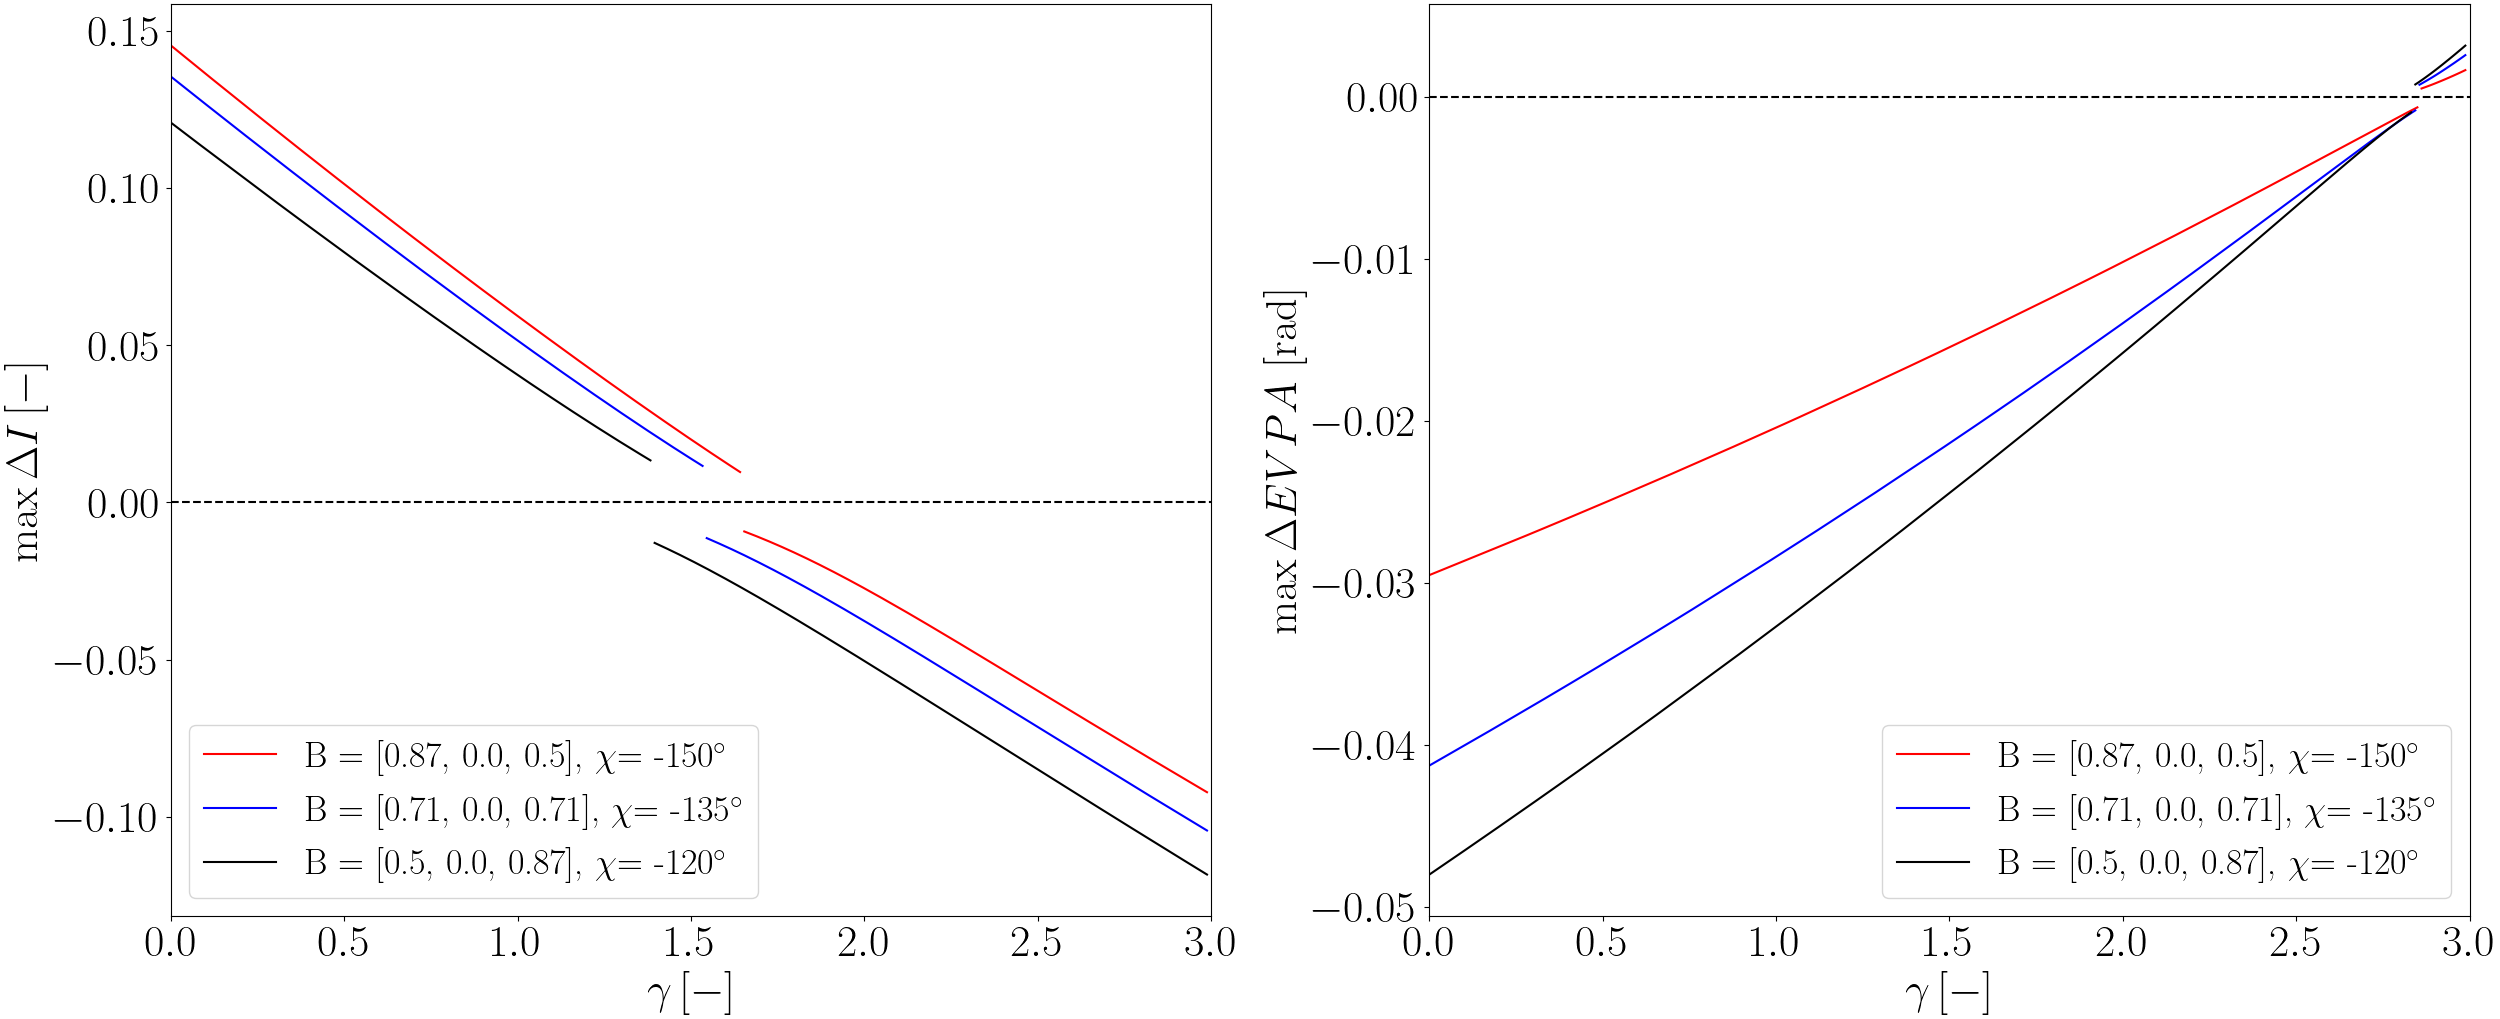
\includegraphics[scale = 0.22]{Section_7_Polarized_Emission/WH_20_deg_param_sweep.png}
		\caption[The maximum deviation of the direct images of type $\{x,y\}\vert_{6M, \text{Schw}}$, for $i = 20\deg$.]{\small
			The maximum deviation in amplitude for the direct polarized images of type $\{x,y\}\vert_{6M, \text{Schw}}$ for $i = 20\deg$. Negative values imply that the corresponding quantity is larger by magnitude for the Schwarzschild black hole.} 
		\label{WH_max_deviation_70_deg}
	\end{figure}
	
	We see that there exist two critical values for $\gamma$ which minimize the deviation in intensity and position angle. This is summarized in table 1. From there we can notice that the minimal deviation for the wormhole at these inclinations can fall below $4\%$. The conclusions which follow from this analysis on the direct images are presented in section \emph{3.3}.
	
	\begin{table}[h!]
		\small
		\begin{center}
			\begin{tabular}{||m{7.5em} | m{5em} | m{5em} | m{7em} | m{3em}| m{2em}||} 
				\hline
				Magnetic field & Quantity to minimize & \small $\frac{\max\Delta I}{I_\text{Schw}}$ [\%]& \small $\frac{\max\Delta EVPA}{EVPA_{\text{Schw}}}$ [\%] & $\phi$ [rad] & $\gamma_\text{crit}$ \\ [0.5ex] 
				\hline\hline
				\multirow{2}{7.5em}{\small $\vec{B} = [0.5, 0, 0.87]$} & \centering $\Delta I$ & \centering 3.8 & \centering 2.2 &  $0.48\pi$ &  1.39\\ 
				& \centering $\Delta EVPA$ & \centering 23.0 & \centering 0.3 &  $0.73\pi$ & 2.85\\ 
				\hline
				\multirow{2}{8em}{\small $\vec{B} = [0.71, 0, 0.71]$} & \centering $\Delta I$ & \centering3.6 & \centering1.8 & $0.53\pi$ & 1.54\\ 
				& \centering $\Delta EVPA$ & \centering23.1 & \centering0.07 & $1.32\pi$ & 2.85 \\ 
				\hline
				\multirow{2}{7.5em}{\small $\vec{B} = [0.87, 0, 0.5]$} & \centering $\Delta I$ & \centering3.3 &\centering 1.1 & $0.53\pi$ & 1.64\\ 
				& \centering $\Delta EVPA$ & \centering23.4 & \centering0.04 & $0.32\pi$ & 2.86 \\  [1ex] 
				\hline
			\end{tabular}
		\end{center}
		\caption[Deviations of the polarized images of type $\{x,y\}\vert_{6M, \text{Schw}}$ for $i = 20\deg$ at the critical values $\gamma_\text{crit}$ for wormholes.]{\small Deviations of the polarized images of type $\{x,y\}\vert_{6M, \text{Schw}}$ for $i = 20\deg$ at the critical values $\gamma_\text{crit}$ for wormholes. The quantities in columns 3 and 4 are evaluated at the same point on the observational plane.}
		\label{Deviations_table_20_deg}
	\end{table}
	
	Let us now examine the \emph{indirect} images - more concretely the case of $n = 1$. They have the property that their apparent position changes drastically with the metric parameter $\gamma$. This has an important consequence: while the direct images of type 
	${x, y}|_{X,Schw}$ exist for every value of $\gamma$, this not true for the indirect ones. In section \emph{6.2.2} and \emph{6.3.2} of the dissertation we have investigated the possible values for $\gamma$ that lead to the formation of indirect images of type ${x, y}|_{X,Schw}$. We show that in the case of the wormhole spacetime they exist for $1.8 \lessapprox \gamma \lessapprox 2.7$, while in the case of the Janis-Newman-Winicour solution, for $0.6 \lessapprox \gamma \le 1$. On figure 3.5 we show again the quantitative analysis of the deviations of these images, for an observational inclination $i = 20^\circ$.
	
	\begin{figure}[!htb]
		\begin{subfigure}{16cm}
			\hspace{-1.0em}
			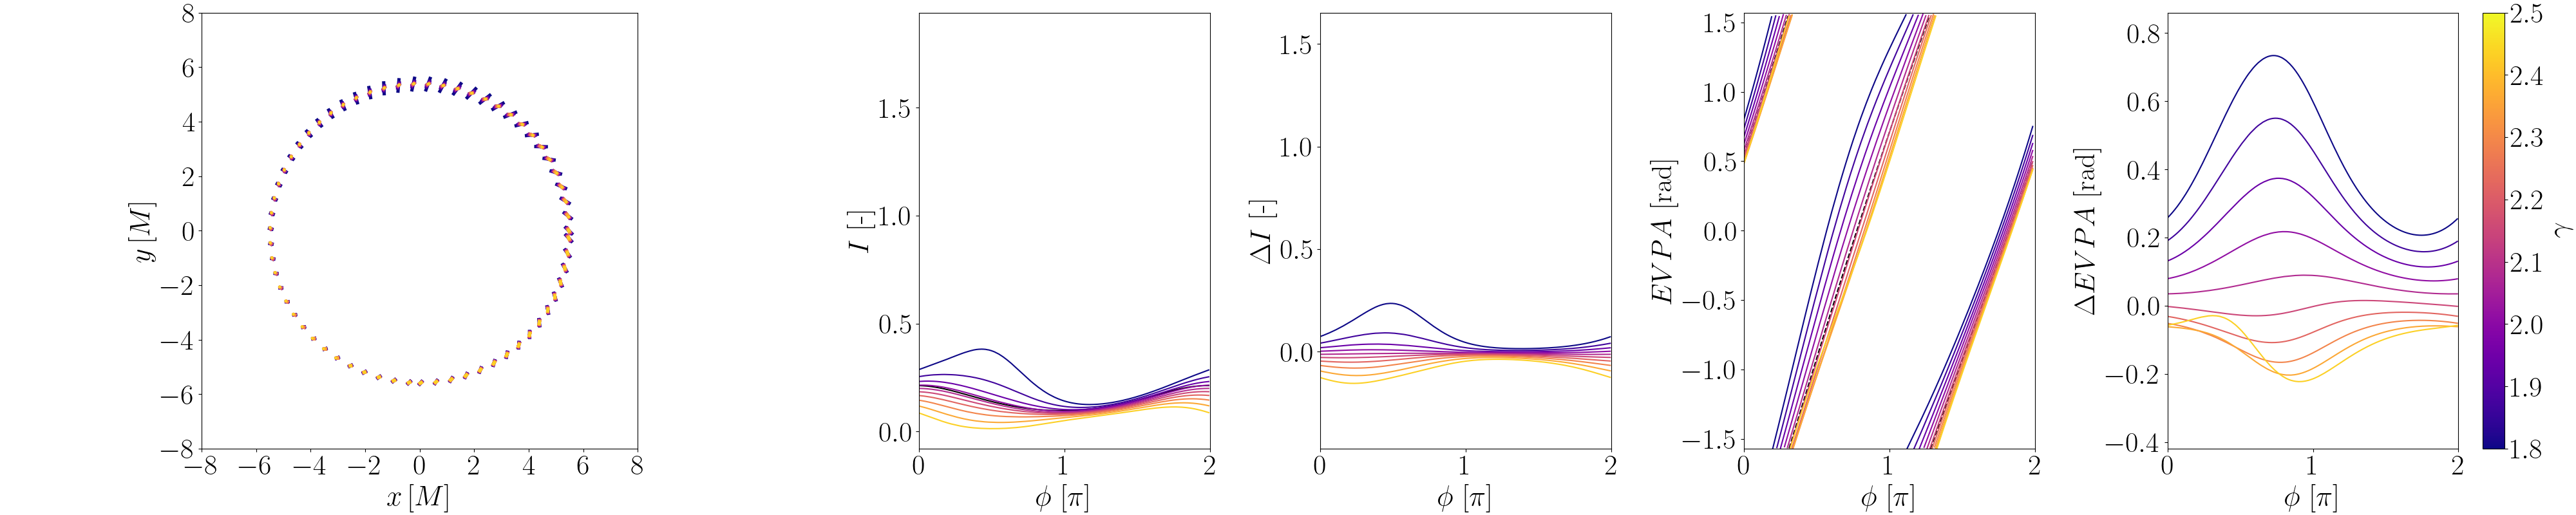
\includegraphics[scale = 0.15]{Section_7_Polarized_Emission/WH_delta_fig_B_0.87_0.5_0_20_deg_r6_n1.png}
			\caption{Wormhole,\\ $\vec{B} = [0.87, 0, 0.5]$, $\beta = 0.3$, $\chi = -150^\circ$, $i = 20^\circ$.} 
		\end{subfigure}\\
		\begin{subfigure}{17cm}
			\hspace{-1.0em}
			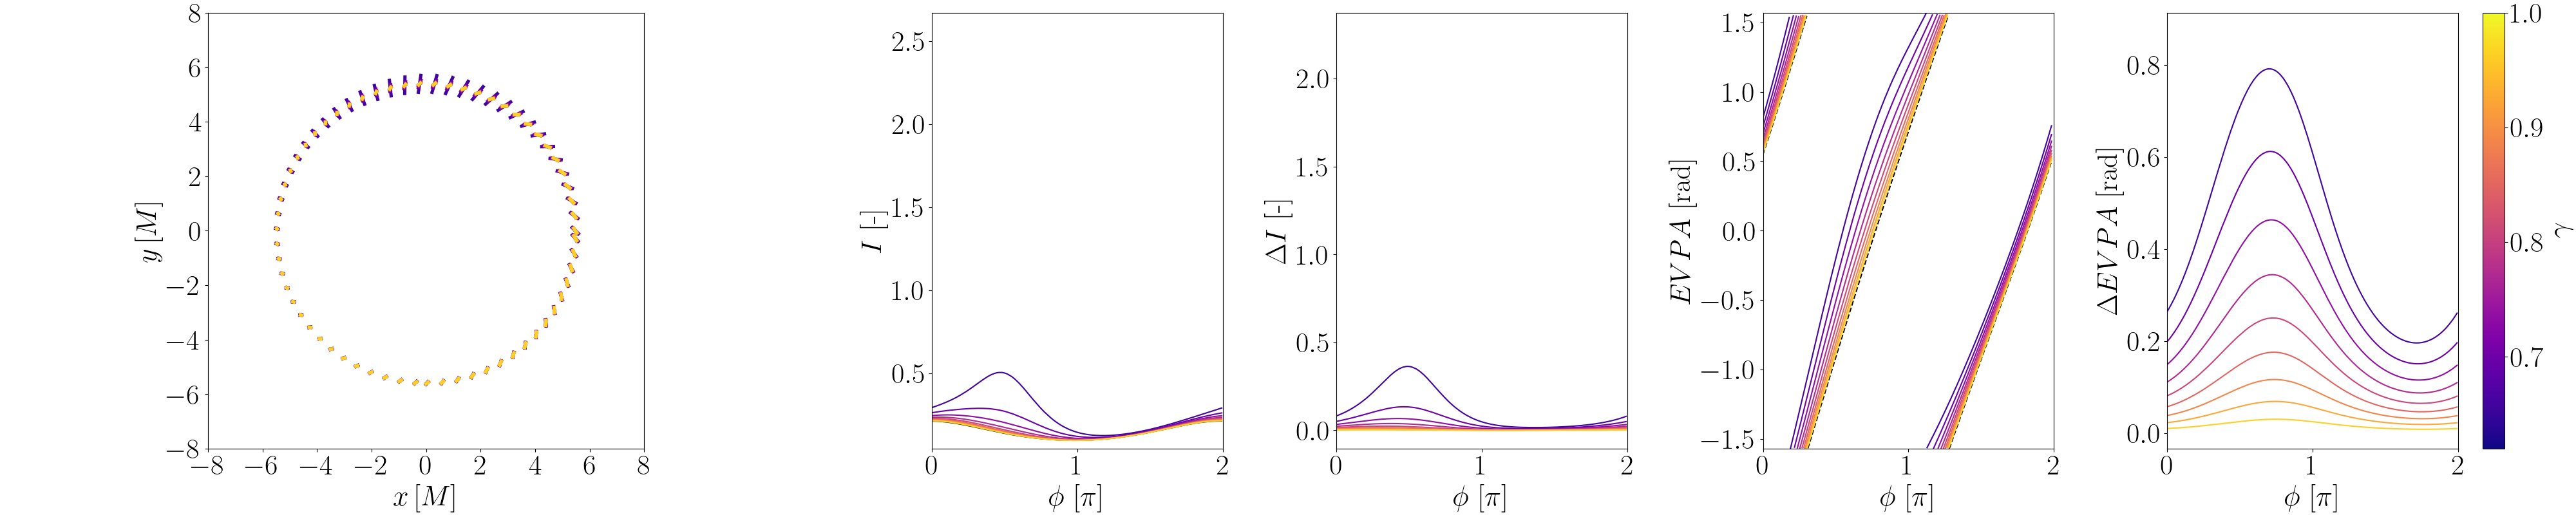
\includegraphics[scale = 0.15]{Section_7_Polarized_Emission/JNW_delta_fig_B_0.87_0.5_0_20_deg_r6_n1.png}
			\caption{Janis-Newman-Winicour naked singularity,\\  $\vec{B} = [0.87, 0, 0.5]$, $\beta = 0.3$, $\chi = -150^\circ$, $i = 20^\circ$.}
		\end{subfigure}
		\caption[The polarized indirect images around wormholes and naked singularities for an equatorial magnetic field at $i = 20^\circ$.]{\small The constructed indirect polarized images of type $\{x,y\}\vert_{6M, \text{Schw}}$ around wormholes and naked singularities at an inclination $i = 20^\circ$. The black curves correspond to a Schwarzschild black hole.} 
		\label{Inirect_image_deltas_20}
	\end{figure}
	
	We see that the strong gravitational lensing effect leads to significant deviations in the images. The maximum deviation in intensity for the wormhole reaches $\max \Delta I_\text{WH} / I_{\text{Schw}} = 650\%$, while for the naked singularity we find$\max \Delta I_\text{JNW} / I_{\text{Schw}} = 6\times10^3\%$!\\
	
	We have to be careful when interpreting these extremely high deviations. The formation of these images for low values of $\gamma$ requires the photons to cross the emission region at very high radial coordinates $r_s\approx 10^3M$, where one would not expect a significant contribution to the emission. It is possible that this compensates the effect of the spacetime and a more realistic model of the emission medium would not produce such spikes in the intensity.\\
	
	Another important signature which we notice is that the intensity distribution shifts towards the top part of the image $\phi = \pi / 2$ with decreasing $\gamma$ for both metrics.
	
	\newpage
	
	\subsection{Conclusion}
	
	Here we studied the linearly polarized images of a thin equatorial accretion disk around ultra-compact objects which do not posses an event horizon. Our goal is to give an estimate for the influence of the ambient spacetime on the observed polarization pattern. With the help of a simplified analytical model of the emission mechanism and the numerical code Mjølnir we simulate the observational quantities of the images of wormhole and naked singularity spacetimes. We focus on the model parameters which best reproduce the observations presented in \cite{EHT_M87_I} - \cite{EHT_M87_VIII}. We thus exclude vertical magnetic fields from our study.\\
	
	We first study the direct images at low inclinations. We show that they do not posses new morphological properties. Due to this we focus on performing a quantitative analysis of their deviations from a Schwarzschild black hole. We show that for all considered values of the metric parameter $\gamma$, for both types of ultra-compact objects, the relative deviation in intensity does not surpass $\approx 43\%$, while that of the position angle does not surpass $3.8\%$. We also show that by fine tuning the value of $\gamma$ for the wormhole, it can reproduce the polarization pattern of a Schwarzschild black hole up to a relative deviation of $4\%$ in both observational quantities, even though this spacetime does not reduce to Schwarzchild for any value of $\gamma$.\\
	
	Increasing the inclination we find that the deviations increase - for the position angle they can reach $25\%$ (in the case of the wormhole spacetime), but their morphology remains qualitatively similar to that of a Schwarzschild black hole. Based on this we can conclude the following:\\
	
	\emph{The direct images of the emission medium are weakly influenced by the nature of the ambient spacetime. The dominating factor, determining their polarization properties is the magnetic field.}\\
	
	After that we considered the indirect images with $n = 1$. We shoed that their relative deviations in intensity from a Schwarzschild black hole can reach more than two orders of magnitude, while those in position angle can surpass $50\%$. We also observe a morphological difference at low $\gamma$ - the apparent position of the intensity maximum shifts to the top of the image $\phi\approx\pi / 2$. From this we can conclude the following:\\
	
	\emph{The indirect polarized images are strongly sensitive to both the nature of the ambient spacetime and the magnetic field.}\\
	
	Here one can raise the question of how feasible is the observational isolation of the $n = 0$ and $n = 1$ images from the rest. Motivated by this question, as well as the possibility of observing the exotic images from chapter \emph{2} (and chapter \emph{5} of the dissertation) we turn our attention in publication IV to simulating realistic observation of the ultra-compact objects described in chapter \emph{4} of the dissertation, with the help of the software packages ehtim and VIDA.
	
	\section{Observing exotic compact objects}
	
	As we mention in publication I, exotic compact objects can generate qualitatively different from black holes images of their emission medium. We also showed in publications II and III that the polarized images with $n = 1$ are strongly influenced by the nature of the ambient spacetime. It is natural to ask the question weather, keeping in mind the current observational techniques, it is possible to experimentally confirm the predictions from the previous two chapters?\\
	
	As of the moment of writing, the only observations of supermassive compact object with a resolution comparable to the size of the relativistic images that have been carried out are the ones by the EHT collaboration. The methodology of said observations and the following reconstruction of images are described in \cite{EHT_M87_II}, \cite{EHT_M87_III}. Here we will focus only on the end result of their procedure - the images. We can notice from \cite{EHT_M87_I}, \cite{EHT_SGR_I} (and out summary in chapter \emph{3} of the dissertation) that the 2017 observations do not have the resolution to distinguish the indirect images from the direct ones. We can then ask the following questions: is it possible trough the observations of the EHT collaboration from 2017 and future such to:\\
	
	\textbf{1)} Unambiguously detect the presence of exotic images of the emission medium?\\
	
	\textbf{2)} To observationally separate the images with $n = 1$ from the rest.\\
	
	To answer these two question we must simulate these observations. the EHT collaboration has developed a software package, called ehtim,\footnote{https://github.com/achael/eht-imaging} \cite{EHTIM}, which does just that. It uses as an input "ideal observations"\footnote{In this context it is important to distinguish between simulated observations, and the images produced from solving the equation of radiative transfer and parallel transport. The first we will refer to as \textbf{reconstructed} and the latter - \textbf{ideal}.} of the objects, a configuration of radio telescopes and parameters for the reconstruction algorithm.\\
	
	To generate the ideal images of ultra-compact objects we use a phenomenological model of a radiativelly inefficient accretion flow (RIAF), presented in section \emph{4.1}, with parameters derived from the 2017 EHT observational campaign (see chapter \emph{3} of the dissertation or \cite{EHT_M87_V}, \cite{EHT_M87_VIII}). The generation itself is done trough solving the system of geodesic equations for the target spacetime, coupled to the equations for radiative transfer. This is done using the numerical code Mjølnir developed by the author\footnote{https://github.com/ValentinDeliyski/Mjolnir\_GRRT}.\\
	
	\noindent We consider three different configuration of radio telescopes, corresponding to the observational campaigns from 2017, 2022 and the planned ngEHT.\\
	
	\noindent The parameters for the reconstruction algorithm we fix following \cite{EHTIM}.\\
	
	\noindent As a last step, we characterize the morphology of the reconstructed images with the help of a template based analysis. This lets us systematically define the region of the central depression, which we observe in \cite{EHT_M87_I}, \cite{EHT_SGR_I}. For this we use the software package VIDA\footnote{https://github.com/ptiede/VIDA.jl} \cite{VIDA}.
	
	
	\subsection{Model of the emission medium}
	
	We will consider a phenomenological model that describes a geometrically and optically thin, radiatively inefficient accretion flow in the so called \emph{magnetically arrested disk (MAD)} state. The model is chosen so that it qualitatively reproduces general relativistic magneto-hydrodynamic (GRMHD) simulations \cite{Yuan2003}. Following \cite{Gold2020}, \cite{Broderick2021} we assume that the emission we observe from M87$^*$ is synchotron in nature, and it due to two distinct ensembles of electrons - a thermal and non-thermal one. We describe their collective sum with a density that has a power law scaling in the radial direction, and a vertical Gaussian profile:
	
	\begin{equation}
		n_e(r,z) = n_0\left(\frac{r}{r_0}\right)^{-2}e^{-\frac{z^2}{2(\alpha\rho)^2}}
		\begin{cases}
			e^{-\frac{(r-r_0)^2}{r^2_{\text{sc}}}},\quad 0 < r < r_0,\\
			1,\,\,\qquad\qquad r>r_0
		\end{cases}
	\end{equation}
	
	Here the parameter $r_0$ determines the position of the peak density of the disk and along with the exponential term appearing when $0 < r < r_0$ serves to fix the position of the apparent emitting region. The cylindrical coordinates $\rho$ and $z$ are given as $\rho = r\sin\theta$, $z = r\cos\theta$ and the parameter $\alpha$ defines the opening angle of the disk $\theta_{\text{op}}$ via $\alpha = \tan\theta_\text{op}$. To generate a thin disk we fix 
	$\alpha = 0.1 \rightarrow \theta_{\text{op}}\approx 5.71^\circ$  for all of our simulations.\\
	In our studies we aim to reproduce the physical conditions under which we observe M87$^*$ and we thus pick $r_0$ and $r_\text{sc}$ such that the diameter of the apparent emitting region is $d_\text{img}\approx 50\, \mu\text{arcsec}$.\\
	
	Along with (4.1) we must also specify a temperature profile:
	
	\begin{equation}
		T_e(r,z) = T_0\left(\frac{r}{r_0}\right)^{-1}
		\begin{cases}
			e^{-\frac{(r-r_0)^2}{r^2_{\text{sc}}}},\quad 0 < r < r_0,\\
			1,\,\,\qquad\qquad r>r_0
		\end{cases}
	\end{equation}
	
	The parameters $n_0$ and $T_0$ which correspond to the equatorial values of the electron number density and temperature at $r = r_\text{sc}$ determine the value of the observed flux. And because both of them are constrained only by the observed flux, we choose to fix $n_0$ and vary $T_0$, so that said flux at 230 GHz is $F_{\text{230 GHz}} \approx 0.5 \text{Jy}$\\
	
	The next step in building up the model is specifying the magnetic field $\vec{B}$. It is most convenient to do this in the rest frame of the fluid, where the emission functions, which we will comment below, are specified. We choose to work in terms of the parameter $\sigma$:
	\begin{equation}
		\sigma = \frac{B^2}{4\pi m_pc^2n_e},
	\end{equation}
	
	where $B$, $m_p$, $c$ and $n_e$ the magnetic field magnitude, proton mass, speed of light and electron number density respectfully, evaluated in \emph{Gaussian units}. To reproduce the 2017 EHT  observations it is enough to assume the disk is \emph{uniformly magnetized} and fix $\sigma = \text{const}$. Following previous works \cite{KERR_SIM_PAPER}, \cite{Geometric_Modeling}, we choose $\sigma = 0.01$. This fixes magnitude of the magnetic field but the synchotron emission we consider is strongly dependent on the geometry of this magnetic field. Never the less, for the purposes of this study the exact orientation of the magnetic field is not important, and we choose to average over all such orientations. In practice this reduces to averaging the emission function over the electron pitch angle  $\alpha = \arccos\frac{\vec{k}\cdot\vec{B}}{|\vec{k}||\vec{B}|}$, where $\vec{k}$ is the local three-wave vector of the photon. We thus do not specify the magnetic field geometry in our study.\\
	
	We assume that the emission can be described in the ultra-relativistic limit (hinted at by the high temperature discussed in section \emph{3} of the dissertation). The reader can find a detailed derivation of this emission mechanism in appendix A of the dissertation. For the purposes of this study we do not consider the polarization of the emitted radiation - only its intensity. We can thus assume the only non-zero source and absorption terms in the radiative transfer equation to be $\{j_{I,\nu}, \kappa_{I,\nu}\}.$ One simplifying assumption which we will adopt (as did the EHT team in \cite{EHT_M87_VIII}) is that the entire electron ensemble is thermal in nature. This assumption influences mainly the derived from observations mass accretion rate $\dot{M}$, which is not relevant to us \cite{EHT_M87_VIII}. We thus assume the following form for $\{j_{I,\nu}, \alpha_{I,\nu}\}$ (see A.62 of the dissertation):
	\begin{subequations}
		\begin{equation}
			j_{I,\nu}\approx n_e \frac{\sqrt{2}\pi e^2\nu_s}{3cK_2(\Theta_e^{-1})}\left(X^{1/2} + 2^{11/12}X^{1/6}\right)^2 e^{-X^{1/3}}
		\end{equation}
		\begin{equation}
			\alpha_{I,\nu} = \frac{j_{I,\nu}}{B_\nu(T)}
		\end{equation}
	\end{subequations}
	Where $B_\nu(T)$ is the Planck function, $\Theta_e = k_BT/mc^2$ and $K_2$ is the modified Bessel function of the second kind. We have additionally introduced the variables:
	\begin{equation}
		X = \frac{\nu}{\nu_s},\quad \nu_s = \frac{2}{9}\nu_\text{cyclo}\Theta_e^2\sin\alpha, \quad \nu_\text{cyclo} = \frac{eB}{2\pi m c}.
	\end{equation}
	It is important to point out that the quantities appearing in (4.4) and (4.5) are evaluated in \emph{Gaussian units}. Then the averaging of (8.4a) is given by:
	\begin{equation}
		j_{I,\nu}\rightarrow\langle j_{I,\nu} \rangle = \frac{1}{4\pi}\int j_{I,\nu} d\Omega = \frac{1}{2}\int j_{I,\nu} \sin\theta d\theta.
	\end{equation}
	The last step in building out the model is specifying a velocity profile for the accretion flow. We follow \cite{Broderick2021}, \cite{Gold2020} and assume a four-velocity of the form:
	\begin{equation}
		u_\mu dx^\mu = u_0(-dt + \ell d\phi),\quad \ell = \frac{\rho^{3/2}}{1 +\rho}
	\end{equation}
	Normalizing $u_\mu$ fixes the value of $u_0$ to:
	\begin{equation}
		u_0 = \frac{1}{\sqrt{-(g^{tt} - 2g^{t\phi}\ell + g^{\phi\phi}\ell^2)}}
	\end{equation}
	When initially running the simulations we found that the form for $\ell$ (4.7) leads to a four-velocity that is not always well defined for the spacetimes we consider. We thus introduce the corrections:
	\begin{equation}
		\ell\rightarrow\begin{cases}
			\ell \left(1 - \frac{2M}{\gamma r}\right)^{\gamma}, \quad\text{for the Janis-Newman-Winicour solution}\\
			\ell \left(1 - \frac{b}{r}\right), \,\,\,\qquad\text{for Wormholes}.
		\end{cases}
	\end{equation}
	
	\subsection{Results}
	
	As we mentioned before, the ideal images we generate with the help of the numerical code Mjølnir. As we wish to reproduce the M87$^*$ observations, we choose an observer inclination $i = 160^\circ$, mass of the compact object $M = 6.2\times 10^9M_\odot$ and the distance to it $D = 16.9\, \text{Mpc}$ \cite{EHT_M87_I}. A full list of the model parameters that are common to all simulations presented here can be found in table \ref{table:Common_ray_tracer_params}.\\
	
	\begin{table}[h!]
		\centering
		\begin{tabular}{||c|c||}
			\hline
			\hline
			\thead{ Parameter }   &\thead{Value} \\
			\hline
			\thead{Compact object Mass $M$}  &  \thead{$6.2\times10^9M_\odot$}\\  
			\hline
			
			\thead{Distance to the compact object $d$} &  \thead{$16.9$ Mpc}\\
			\hline
			
			\thead{Disc opening angle ($\alpha = \tan\theta_{\text{op}}$)}  & \thead{0.1}\\
			\hline
			
			\thead{Electron number density $n_0$ at $r = r_0,\,\theta = \frac{\pi}{2}$}  & \thead{5$\times10^2$cm$^{-3}$}\\
			\hline
			
			\thead{Disc magnetization $\sigma$}  & \thead{0.01}\\
			\hline
			
			\thead{Sharpness parameter $\,r_\text{sc}$} & \thead{0.4M}\\
			\hline
			
			\thead{Observer inclination $i$}  & \thead{160$^\circ$}\\
			\hline
			
			\thead{Resolution} & \thead{$1024\times1024$}\\
			\hline
			
			\thead{Field of view} &  \thead{$100\times100\,\,\mu\text{arc}\sec$}\\
			\hline
			\hline
		\end{tabular}
		\caption[Common parameters for all ray-tracing simulations.]{Common parameters for all ray-tracing simulations.}
		\label{table:Common_ray_tracer_params}
	\end{table}
	
	\subsection{Simulated ideal images of M87$^*$}
	
	\noindent First we simulate classic Kerr black holes, which we use as a baseline for comparing with the exotic compact objects. We consider the effect of rotation by performing simulations for spin parameters $a = \{0, 0.5\}$. We find that the images for these two cases are practically identical. We thus show here only the results for the $a = 0$ case\footnote{The $a = 0.5$ case can be found in section \emph{7.2} of the dissertation.} on figure 8.1, where we also plot the brightness temperature along the $\delta_{\text{rel}} = 0$ of the image. While on figure 4.2 we plot the results for the 4D static and spherically symmetric Gauss-Bonnet naked singularity (see chapter \emph{4} of the dissertation) and the Janis-Newman-Winicour naked singularity for chosen values of their metric parameter $\gamma$.\\
	
	We see that the intensity of the central images is significant. It even represent the maximum of the whole image for the Jnis-Newman-Winicour naked singularity, while for the Gauss-Bonnet solution it is only slightly smaller than the maximum. Even if resolving these central images via EHT observations proves difficult, their significant flux would definitely leave an imprint on the reconstructed images. In the next sections we will give a quantitative measure of this effect.
	
	\newpage
	
	\begin{figure}[h!]
		\centering
		\begin{subfigure}{12cm}
			\hspace{-0cm}
			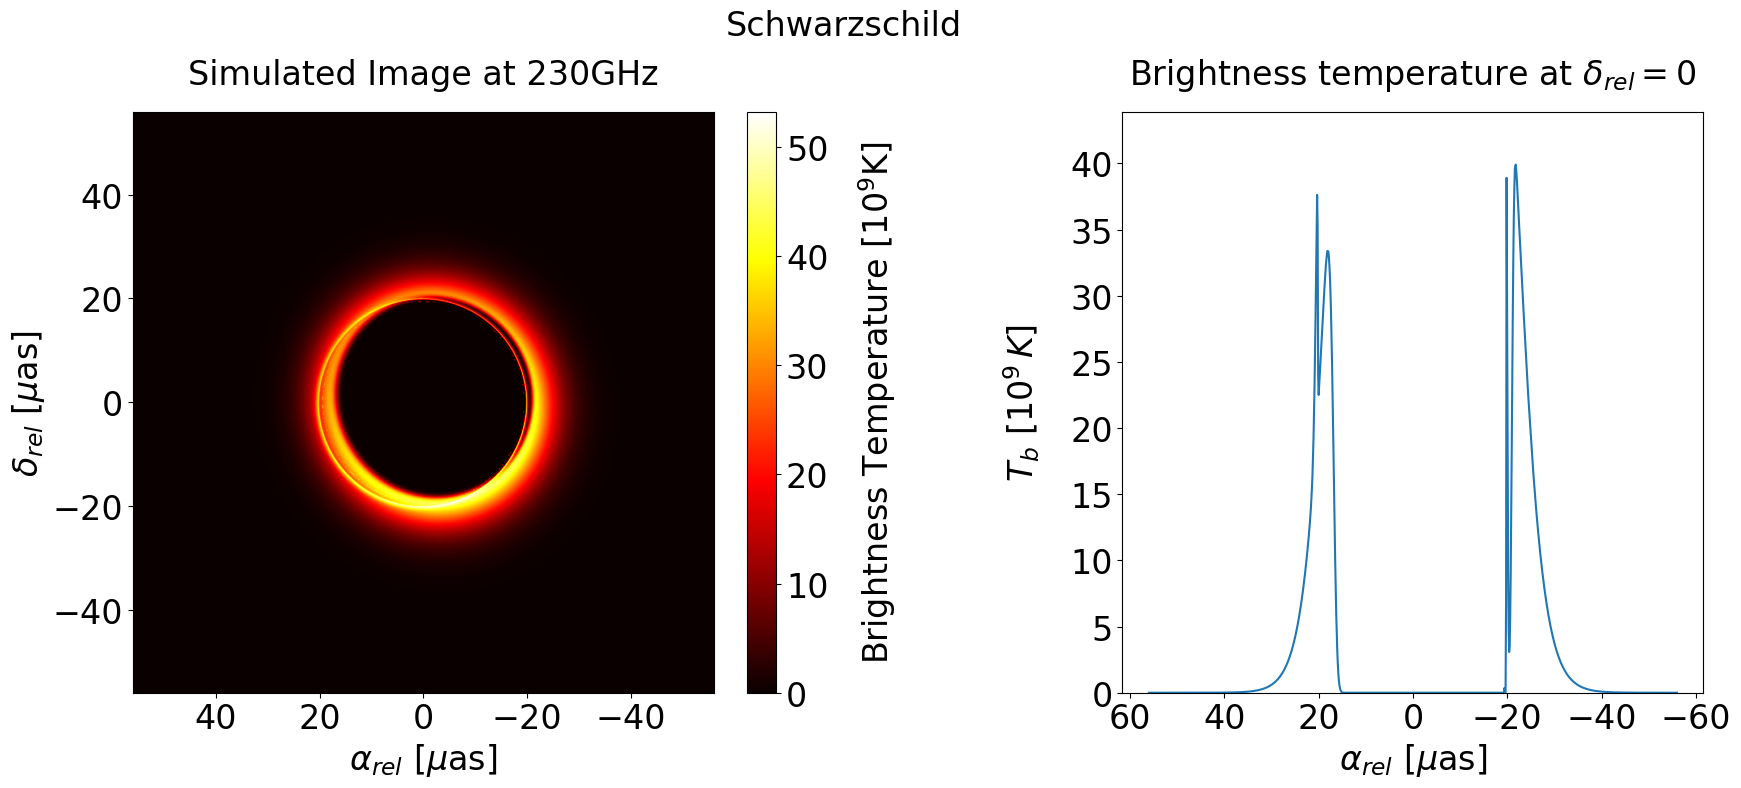
\includegraphics[scale = 0.25]{Section_8_Observing_Horizonless_Objects/Ray_tracer_plot_230_Sch.png}
		\end{subfigure}\\
		\label{Kerr_Ray_tracer_230}
		\caption[Ideal images of a Schwarzschild black hole using a realistic model of the emission medium, at an observation frequency $\nu_\text{obs} = 230$ GHz.]{\small deal images of a Schwarzschild black hole using a realistic model of the emission medium, at an observation frequency $\nu_\text{obs} = 230$ GHz.The temperature at $r = r_0,\,\,\theta = \frac{\pi}{2}$ is fixed to $T_0 = 6.8\times10^{10}$ K and $r_0 = 4.5M$. The total flux is $\mathcal{F}_{\text{tot}} = 0.574$ Jy. For the other model parameters refer to table \ref{table:Common_ray_tracer_params}.} 
	\end{figure}
	
	\begin{figure}[h!]
		\centering
		\begin{subfigure}{12cm}
			\hspace{-0cm}
			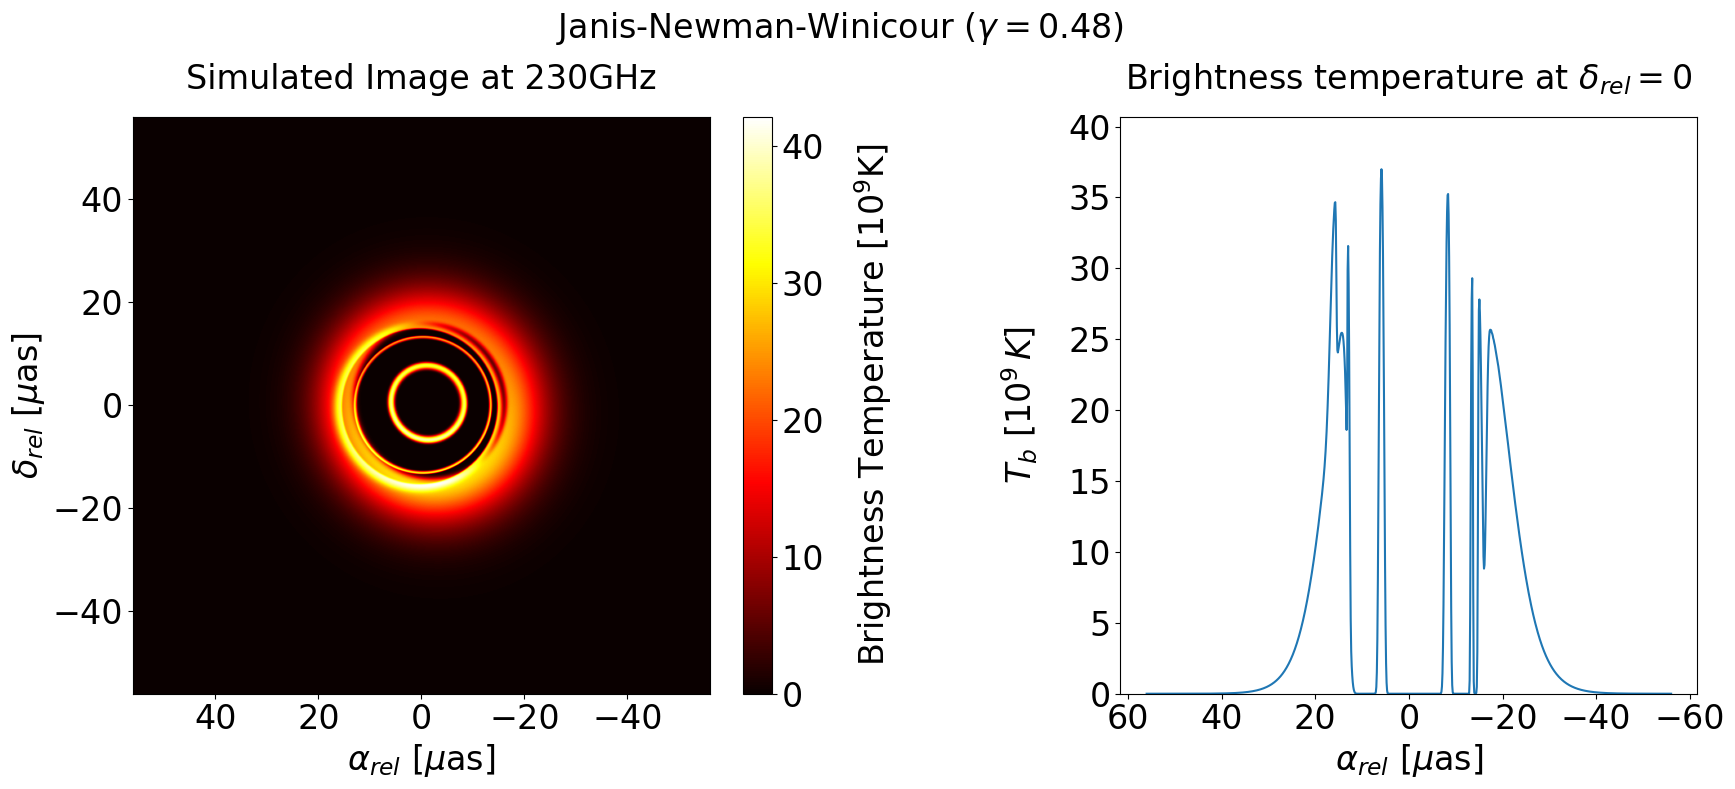
\includegraphics[scale = 0.25]{Section_8_Observing_Horizonless_Objects/Ray_tracer_plot_230_JNW.png}
		\end{subfigure}\\
		\begin{subfigure}{12cm}
			\hspace{-0cm}
			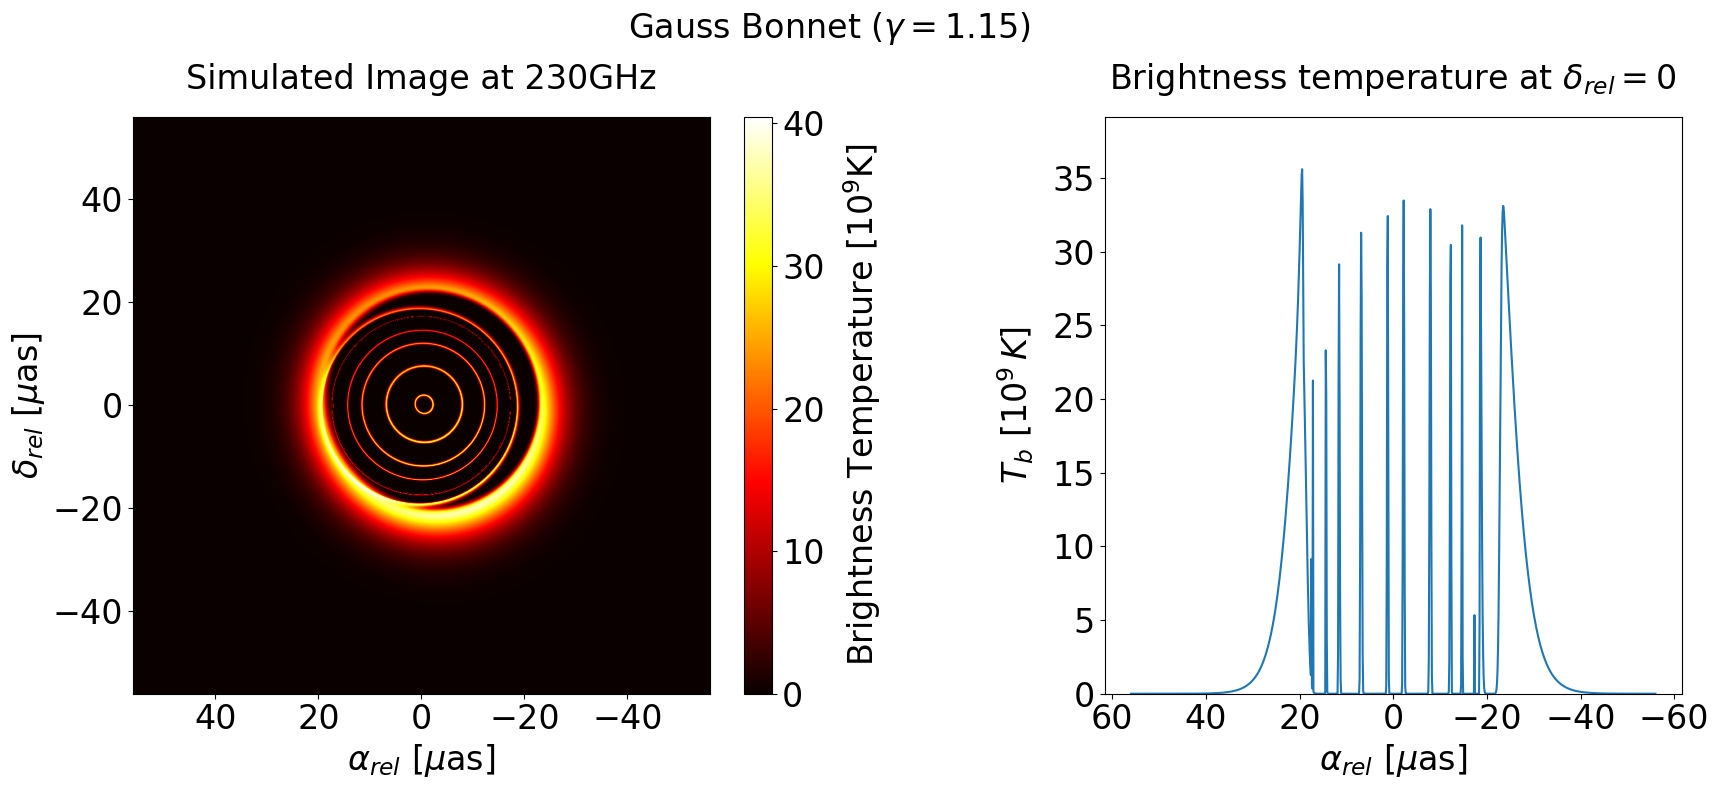
\includegraphics[scale = 0.25]{Section_8_Observing_Horizonless_Objects/Ray_tracer_plot_230_GB.png}
		\end{subfigure}\\
		\label{Naked_Singularity_Ray_tracer_230}
		\caption[Ideal images of naked singularities using a realistic model of the emission medium, at an observation frequency $\nu_\text{obs} = 230$ GHz.]{\small Ideal images of naked singularities using a realistic model of the emission medium, at an observation frequency $\nu_\text{obs} = 230$ GHz, at chosen values for $\gamma$ and an observational frequency $\nu_\text{obs} = 230$ GHz. The temperature at $r = r_0,\,\,\theta = \frac{\pi}{2}$ for the Janis-Newman-Winicour solution is $T_0 = 7.2\times10^{10}$ K, while for the Gauss-Bonnet one it is $T_0 = 5.9\times10^{10}$. The total flux is $\mathcal{F}_{\text{tot}} = 0.574$ Jy and $\mathcal{F}_{\text{tot}} = 0.582$ Jy respectfully. The parameter $r_0$ is fixed to $r_0 = 5M$ for both solutions. For the other model parameters refer to table \ref{table:Common_ray_tracer_params}.} 
	\end{figure}
	
	\subsubsection{Reconstruction of images}
	
	As we already mentioned, we use the library ehtim for the reconstruction of the images of the compact objects in figures 4.1 and 4.2. The methodology behind said reconstructions is discussed in detail in \cite{EHTIM}. Here we will only summarized the settings we use in ehtim - the parameters of the simulated observations, and those of the reconstruction algorithm. After that we comment on our results.\\ 
	
	We consider three radio telescope configurations - those of the 2017 and 2022 EHT observation campaigns, and that of the planned ngEHT. The first two observe only at a frequency of 230 GHz, while ngEHT adds a second one at 345 GHz. The physical parameters of the radio telescopes are tabulated in publication IV.\\
	
	We first use ehtim to generate the so called \emph{synthetic observation}. It consists of the $(u,v)$ coverage of a real observation and has the following input parameters: the integration time $\Delta t$, time between integrations $T$, duration of the observation $T_\text{obs}$ and bandwidth $\Delta\nu$. We choose these parameters based on \cite{EHTIM}, and summarize them in table \ref{table:ehtim_obs_settings}.\\ 
	
	\begin{minipage}{18em}
		\begin{center}
			\begin{tabular}{|| m{7.5em} | m{5em} | m{2em} ||}
				\hline 
				Telescope configuration & \multicolumn{2}{m{7em}||}{Parameters of the synthetic observations} \\
				\hline
				\multirow{4}{7.5em}{\centering \small EHT 2017 / 2022} &\centering $\Delta t,\, [s]$    		& 5   \\ 
				&\centering $T,\,[s]$ 		     		& 30  \\ 
				&\centering $T_\text{obs},\,[h]$ 		& 24  \\
				&\centering $\Delta \nu,\,[\text{GHz}]$ & 4 \\
				\hline
				\multirow{4}{7.5em}{\centering \small ngEHT} 		  & \centering $\Delta t,\, [s]$    	   & 120 \\ 
				& \centering $T,\,[s]$ 		      	   & 600 \\ 
				& \centering $T_\text{obs},\,[h]$ 	   & 24  \\
				& \centering $\Delta \nu,\,[\text{GHz}]$ & 2 \\
				\hline
			\end{tabular}
		\end{center}
		\captionof{table}[Parameters of the synthetic observations.]{Parameters of the synthetic observations.}
		\label{table:ehtim_obs_settings}
	\end{minipage}\,\,
	\begin{minipage}{18em}
		
		The parameters of the reconstruction algorithm we again follow \cite{EHTIM}. We choose to work with the following two data terms: $\chi^2_\text{amp}$ and $\chi^2_\text{cl. phase}$. We then choose the following regularization functions: $S_\text{entropy}$, $S_\text{TSV}$, $S_\text{tot flux}$ and $S_\text{centroid}$. The values for the hyperparameters $\alpha_D$ and $\beta_R$, as well as the number of imaging states and iterations are summarized in table \ref{table:reconstruction_settings}. With the goal of aiding the convergence of the algorithm, we convolve the output image from each imaging stage with a Gaussian pulse, having a standard deviation $\sigma = f_\text{blur} \sigma_{\text{230 GHz}}$, where $\sigma_{\text{230 GHz}}$ is the nominal array resolution at 230 GHz.
	\end{minipage}
	
	\begin{table}[h!]
		\centering
		\begin{tabular}{||c|c|c|c|c|c|c|c|c||}
			\hline
			\hline
			\thead{ Stage } & \thead{$f_\text{blur}$} &\thead{$\beta_\text{entropy}$} &\thead{$\beta_\text{TSV}$} &\thead{$\beta_\text{tot flux}$} & $\beta_\text{centroid}$
			& \thead{$\alpha_\text{amp}$} & \thead{$\alpha_{\text{cl. phase}}$} & $N_\text{iter}$\\
			\hline
			\thead{1}  &  \thead{NA} & \thead{1} &\thead{1} &\thead{100} & \thead{100} &\thead{100} &\thead{200} &\thead{1000} \\  
			\hline
			
			\thead{2}  &  \thead{0.75} & \thead{1} &\thead{50} &\thead{50} & \thead{50} &\thead{100} &\thead{75} &\thead{3000} \\  
			\hline
			
			\thead{3}  &  \thead{0.5} & \thead{1} &\thead{100} &\thead{10} & \thead{10} &\thead{100} &\thead{50} &\thead{4000} \\  
			\hline
			
			\thead{4}  &  \thead{0.33} & \thead{1} &\thead{500} &\thead{1} & \thead{1} &\thead{100} &\thead{100} &\thead{4000} \\  
			\hline
			\hline
			
		\end{tabular}
		\caption[Parameters of the reconstruction algorithm.]{Parameters of the reconstruction algorithm.}
		\label{table:reconstruction_settings}
	\end{table}
	
	\newpage
	
	\noindent The final image we again convolve with a Gaussian pulse that has $\sigma = \sigma_\text{clean} / 2$, where $\sigma_\text{clean}$ is the standard deviation of the "clean beam". This is done to counteract the tendency of this type of algorithm to produce an image with a resolution far greater than that of the actual telescope array.\\
	
	\subsubsection{Reconstructions from EHT 2017}
	
	On figures 4.3 and 4.4 we show the reconstructed images from the simulated observations of the objects presented in figures 4.1 and 4.2. For each reconstructed image we give the final values for $\chi^2_\text{amp}$ and $\chi^2_\text{cl. phase}$. We find that the reconstructions from both sets of telescope arrays (EHT 2017 and EHT 2022) are very similar and thus only show the 2017 ones here\footnote{An exception to this is the Janis-Newman-Winicour naked singularity, which shows a slight morphological difference in the reconstructions. We refer the reader to section \emph{7.3.1} of the dissertation.}, but the quantitative analysis we perform will be shown for both arrays in section \emph{4.4}.
	
	\begin{figure}[h!]
		\centering
		\begin{subfigure}{12cm}
			\hspace{-1.5cm}
			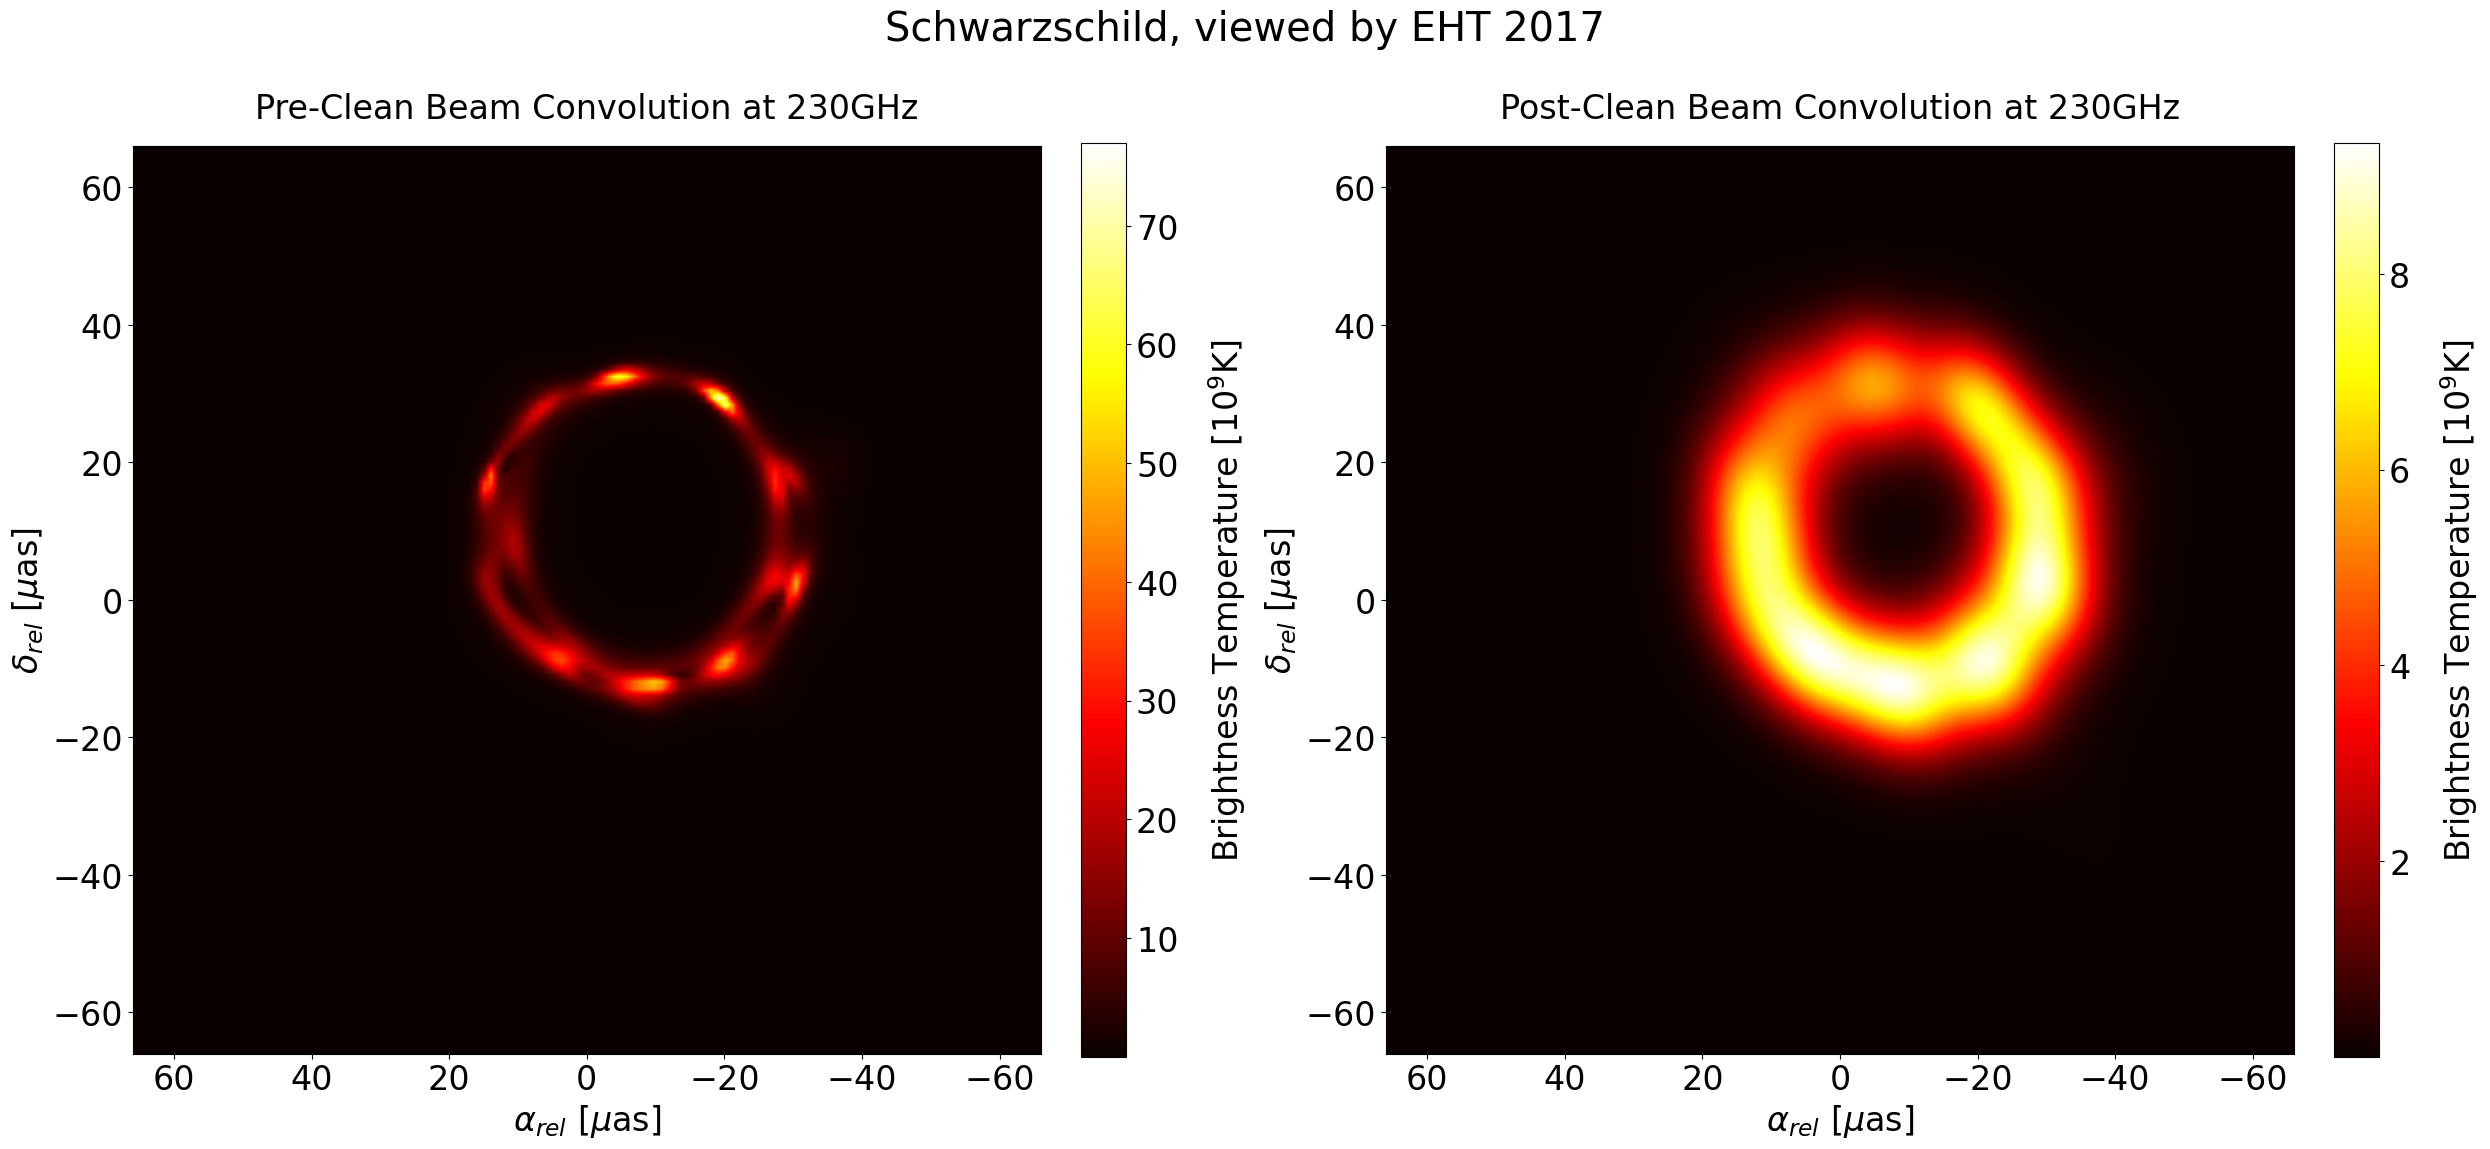
\includegraphics[scale = 0.23]{Section_8_Observing_Horizonless_Objects/Ehtim_plot_2017_no_blur_Sch.png}
		\end{subfigure}\\
		\label{Kerr_EHT_2017}
		\caption[Reconstructed images of Schwarzschild black holes from EHT 2017.]{\small Reconstructed images of Schwarzschild black holes from EHT 2017. The left panel shows the "bare" reconstruction, before convolving it with the "clean beam". The final values for $\chi^2$ are $\chi^2_\text{amp} = 1.02$ and $\chi^2_\text{cl. phase} = 0.9$.} 
	\end{figure}
	
	We see from figure 4.4 that the effective resolution of the telescope array at 230 GHz is not sufficient to discern the presence of exotic images. They get "washed out" and merge with the rest. What we also notice is that this leads to a significant increase in the flux of the central depression. We can thus quantitatively estimate this flux and define from it a measure, based on which to judge the presence of exotic images.
	
	\newpage
	\begin{figure}[h!]
		\centering
		\begin{subfigure}{12cm}
			\hspace{-1.5cm}
			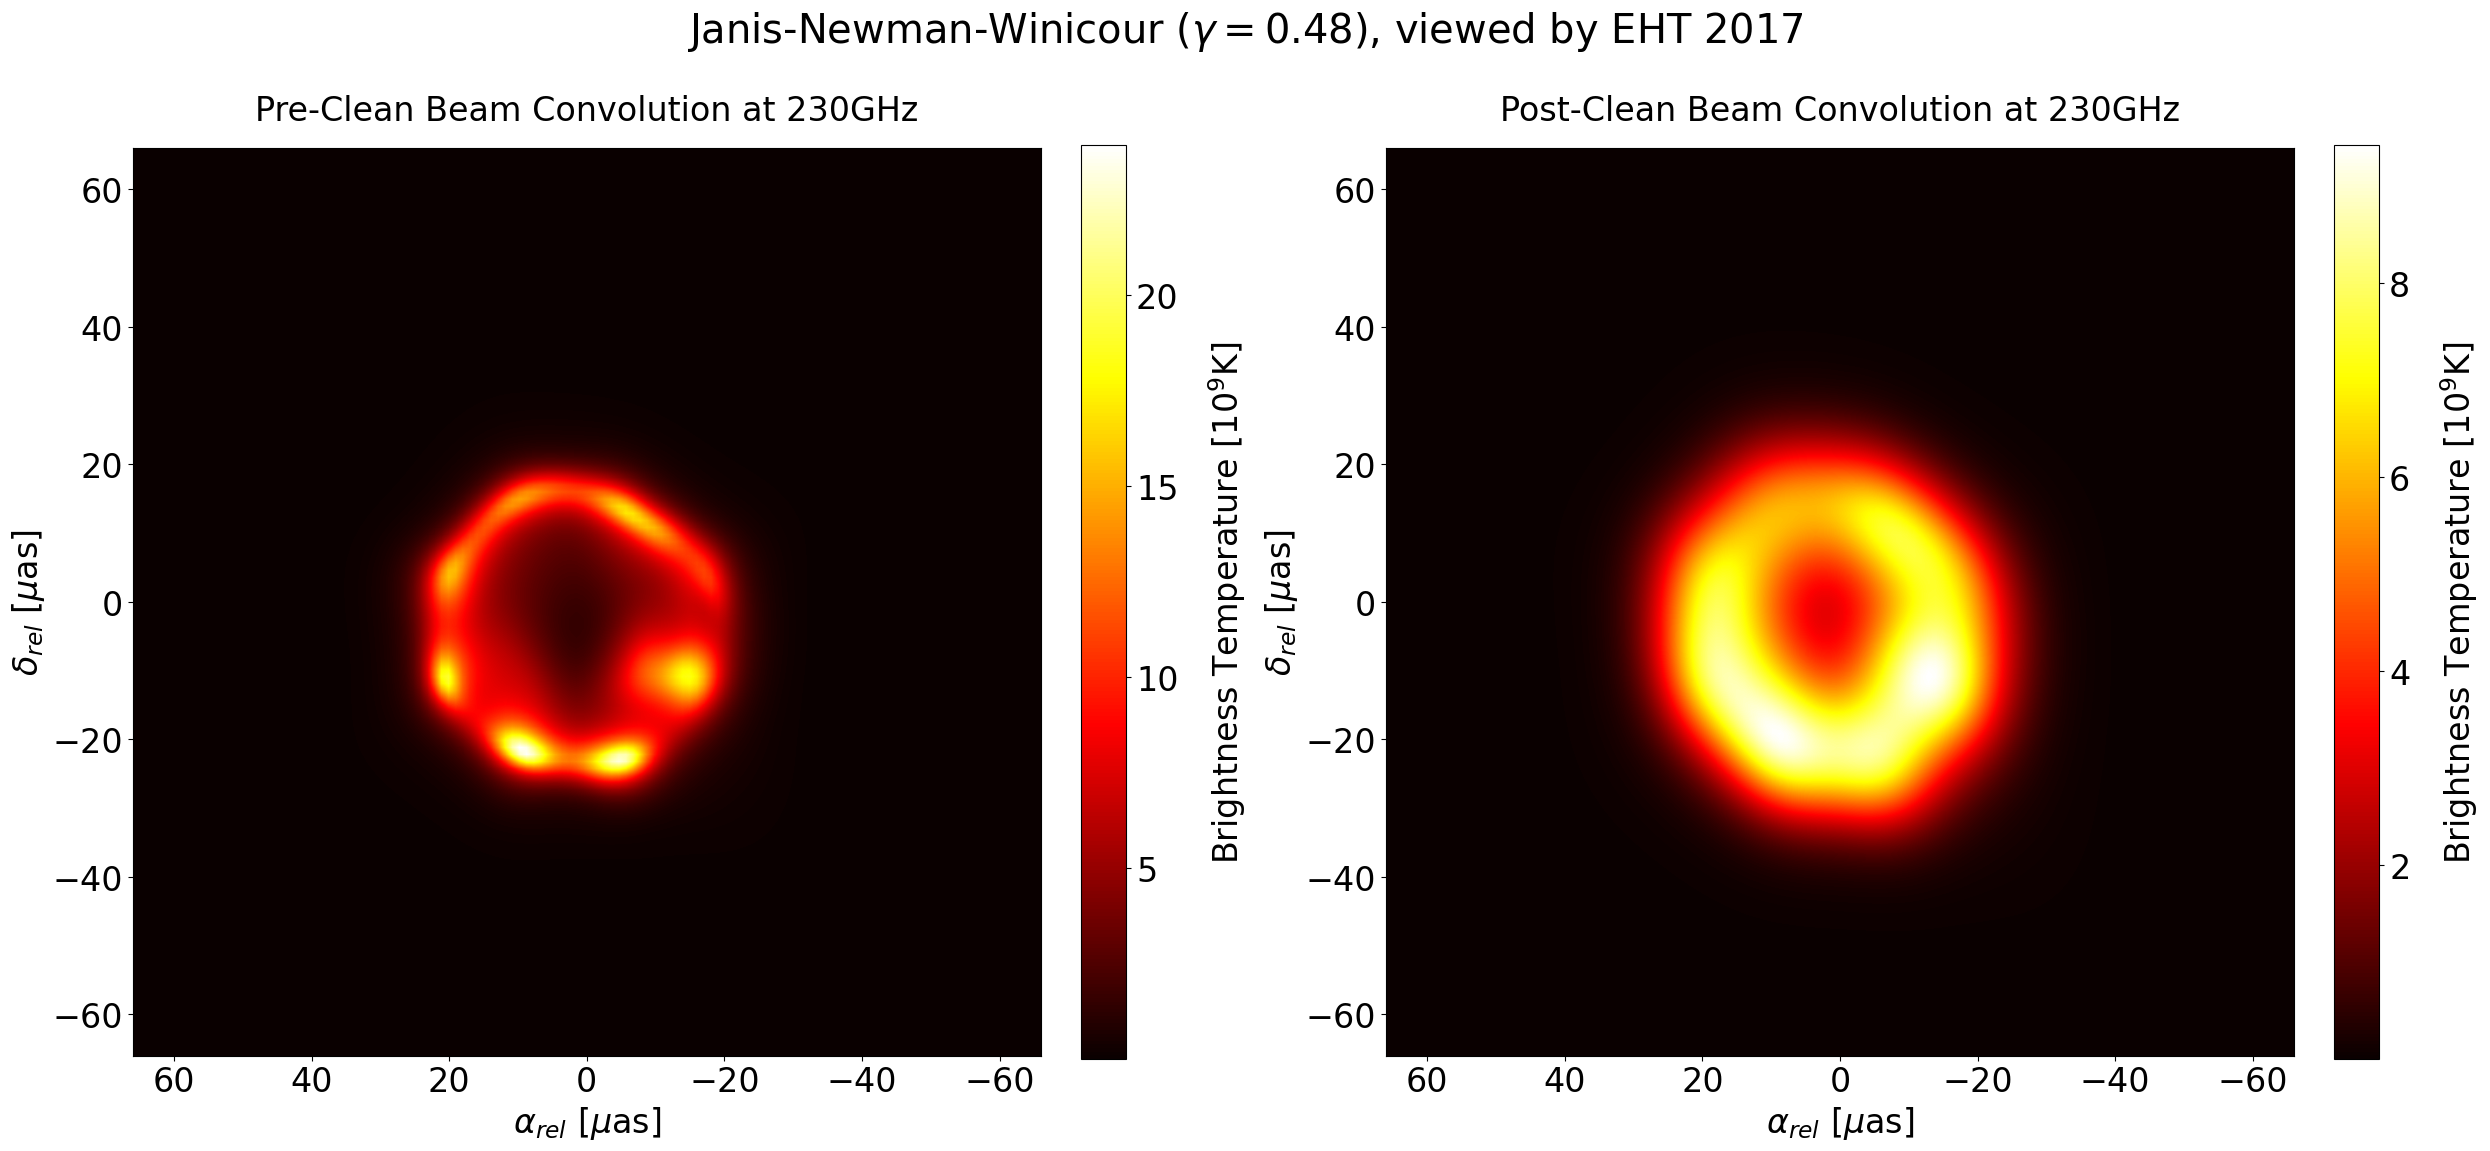
\includegraphics[scale = 0.23]{Section_8_Observing_Horizonless_Objects/Ehtim_plot_2017_no_blur_JNW.png}
		\end{subfigure}\\
		\begin{subfigure}{12cm}
			\hspace{-1.5cm}
			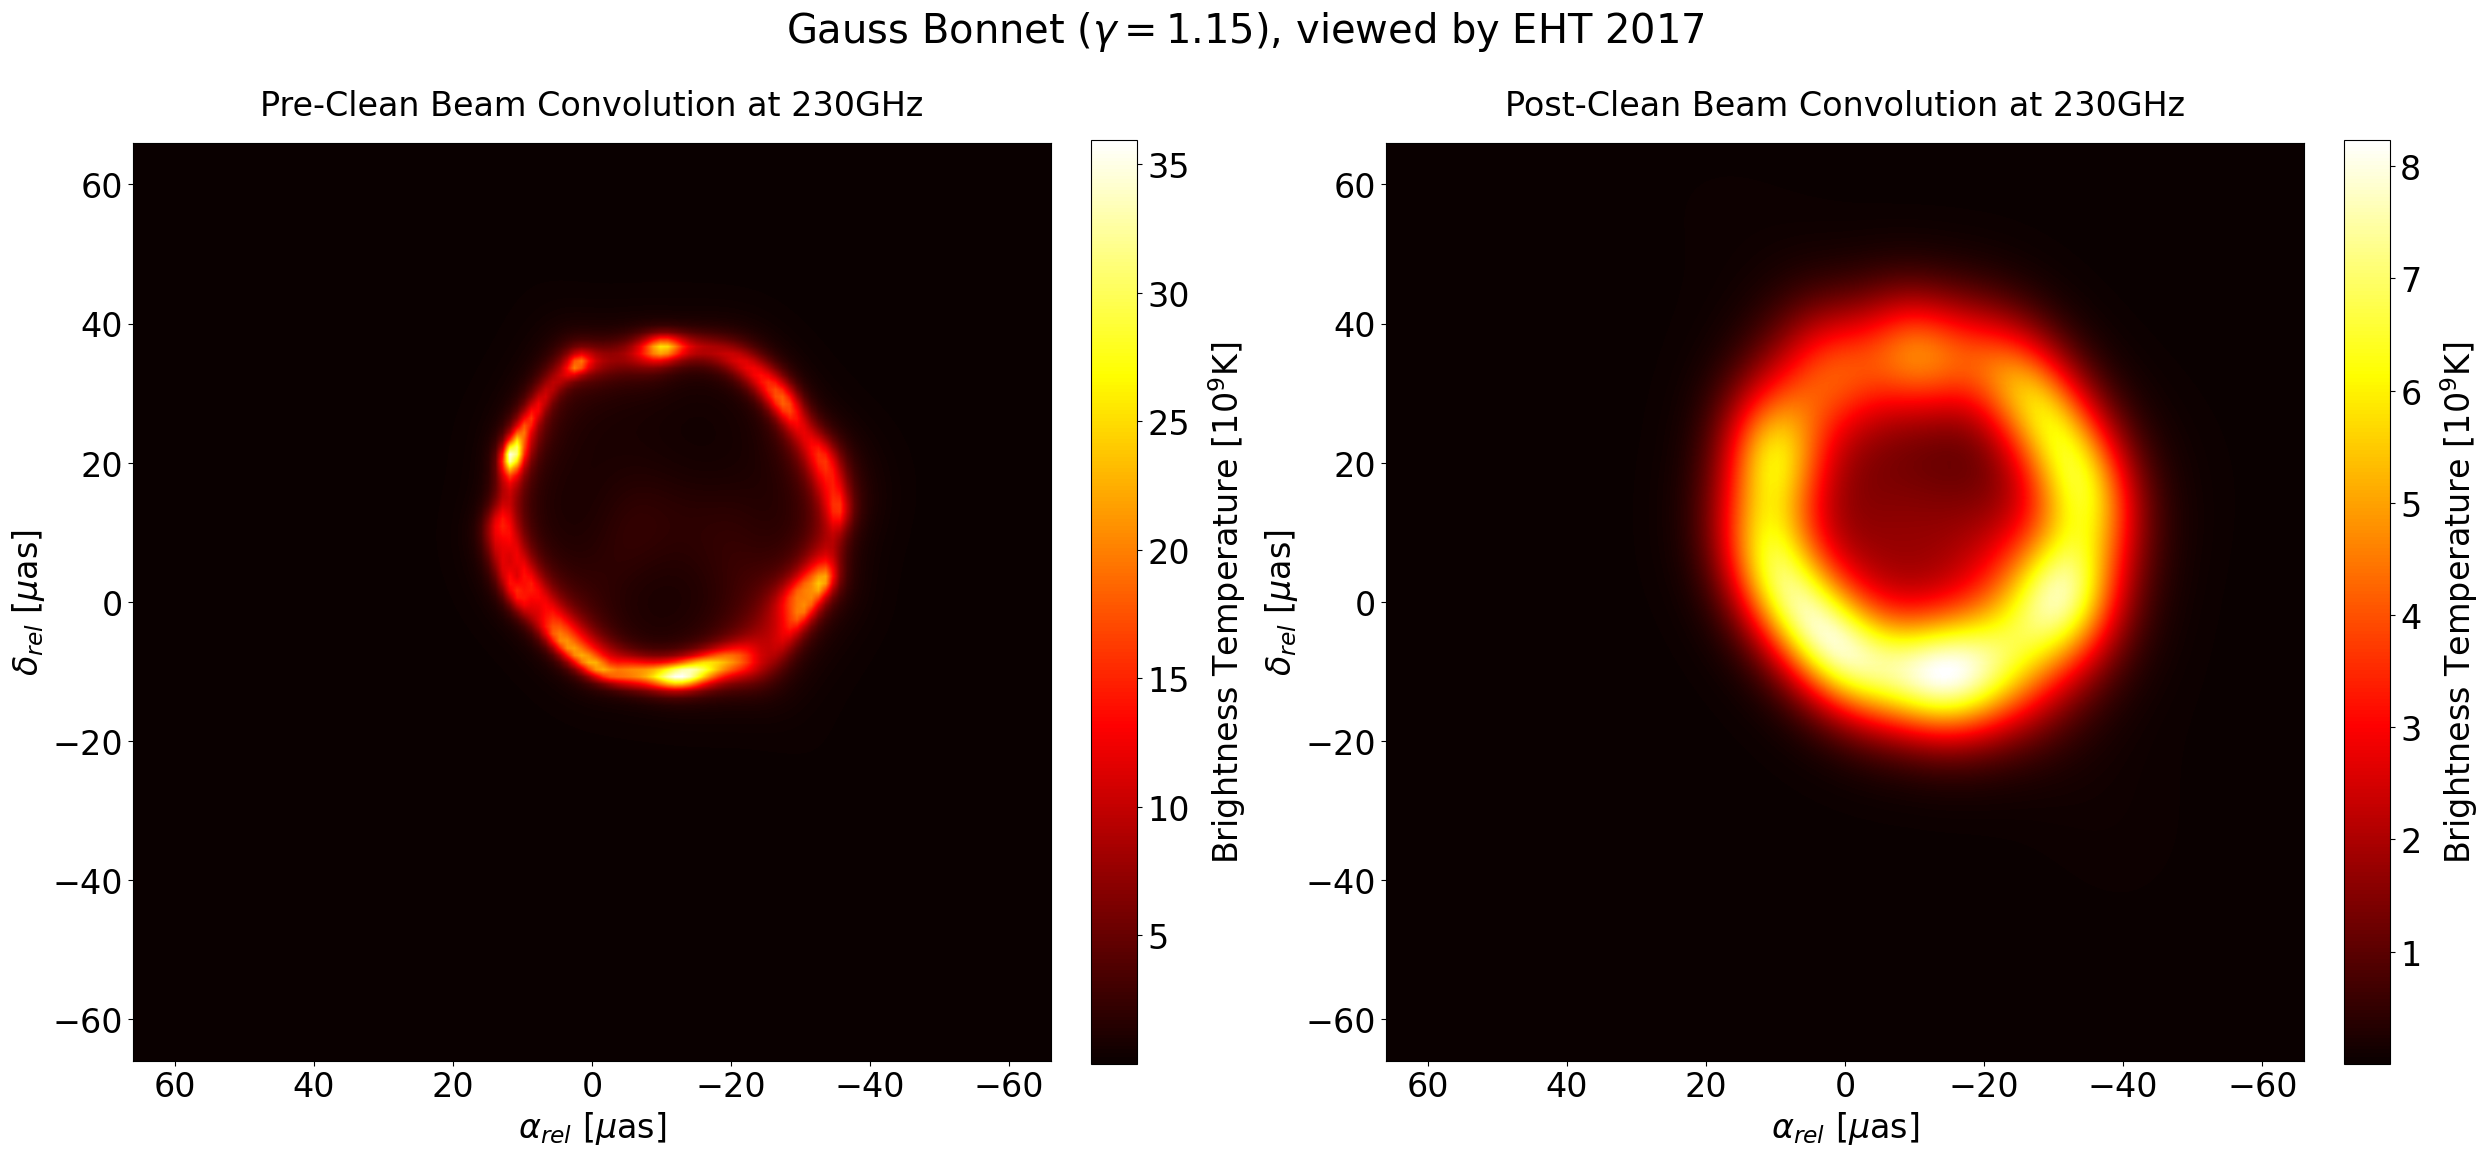
\includegraphics[scale = 0.23]{Section_8_Observing_Horizonless_Objects/Ehtim_plot_2017_no_blur_GB.png}
		\end{subfigure}\\
		\label{Naked_Singularity_EHT_2017}
		\caption[Reconstructed images of naked singularities for chosen values of $\gamma$ from EHT 2017.]{\small Reconstructed images of naked singularities for chosen values of $\gamma$ from EHT 2017. The left panel show the "bare" reconstruction, before convolving it with the "clean beam". The final values for $\chi^2$ are $\chi^2_\text{amp} = \{1.01, 1.00\}$ and $\chi^2_\text{cl. phase} = \{0.91, 0.84\}$ for Gauss-Bonnet and Janis-Newman-Winicour respectfully.} 
	\end{figure}
	
	\subsubsection{Reconstructions from ngEHT}
	
	The perspective future observations of ngEHT will not only have an expanded telescope array (we have considered 21 different sites), but will also add a second, higher observation frequency $\nu = 345$ GHz. The extended array will improve the $(u,v)$ coverage of the observations but it is expected that the second frequency will dramatically increase the effective resolution of the array. On figure 4.5 we show the reconstructions of equivalent simulations to those presented in figure 4.2, only at 345 GHz. We see that even though the morphology of the exotic images is will not resolved, the observations at 345 GHz become sensitive to them. We find a clear local maximum inside the central depression. In the next section we will give a quantitative account of this depression.
	
	\begin{figure}[h!]
		\centering
		\begin{subfigure}{12cm}
			\hspace{-1.5cm}
			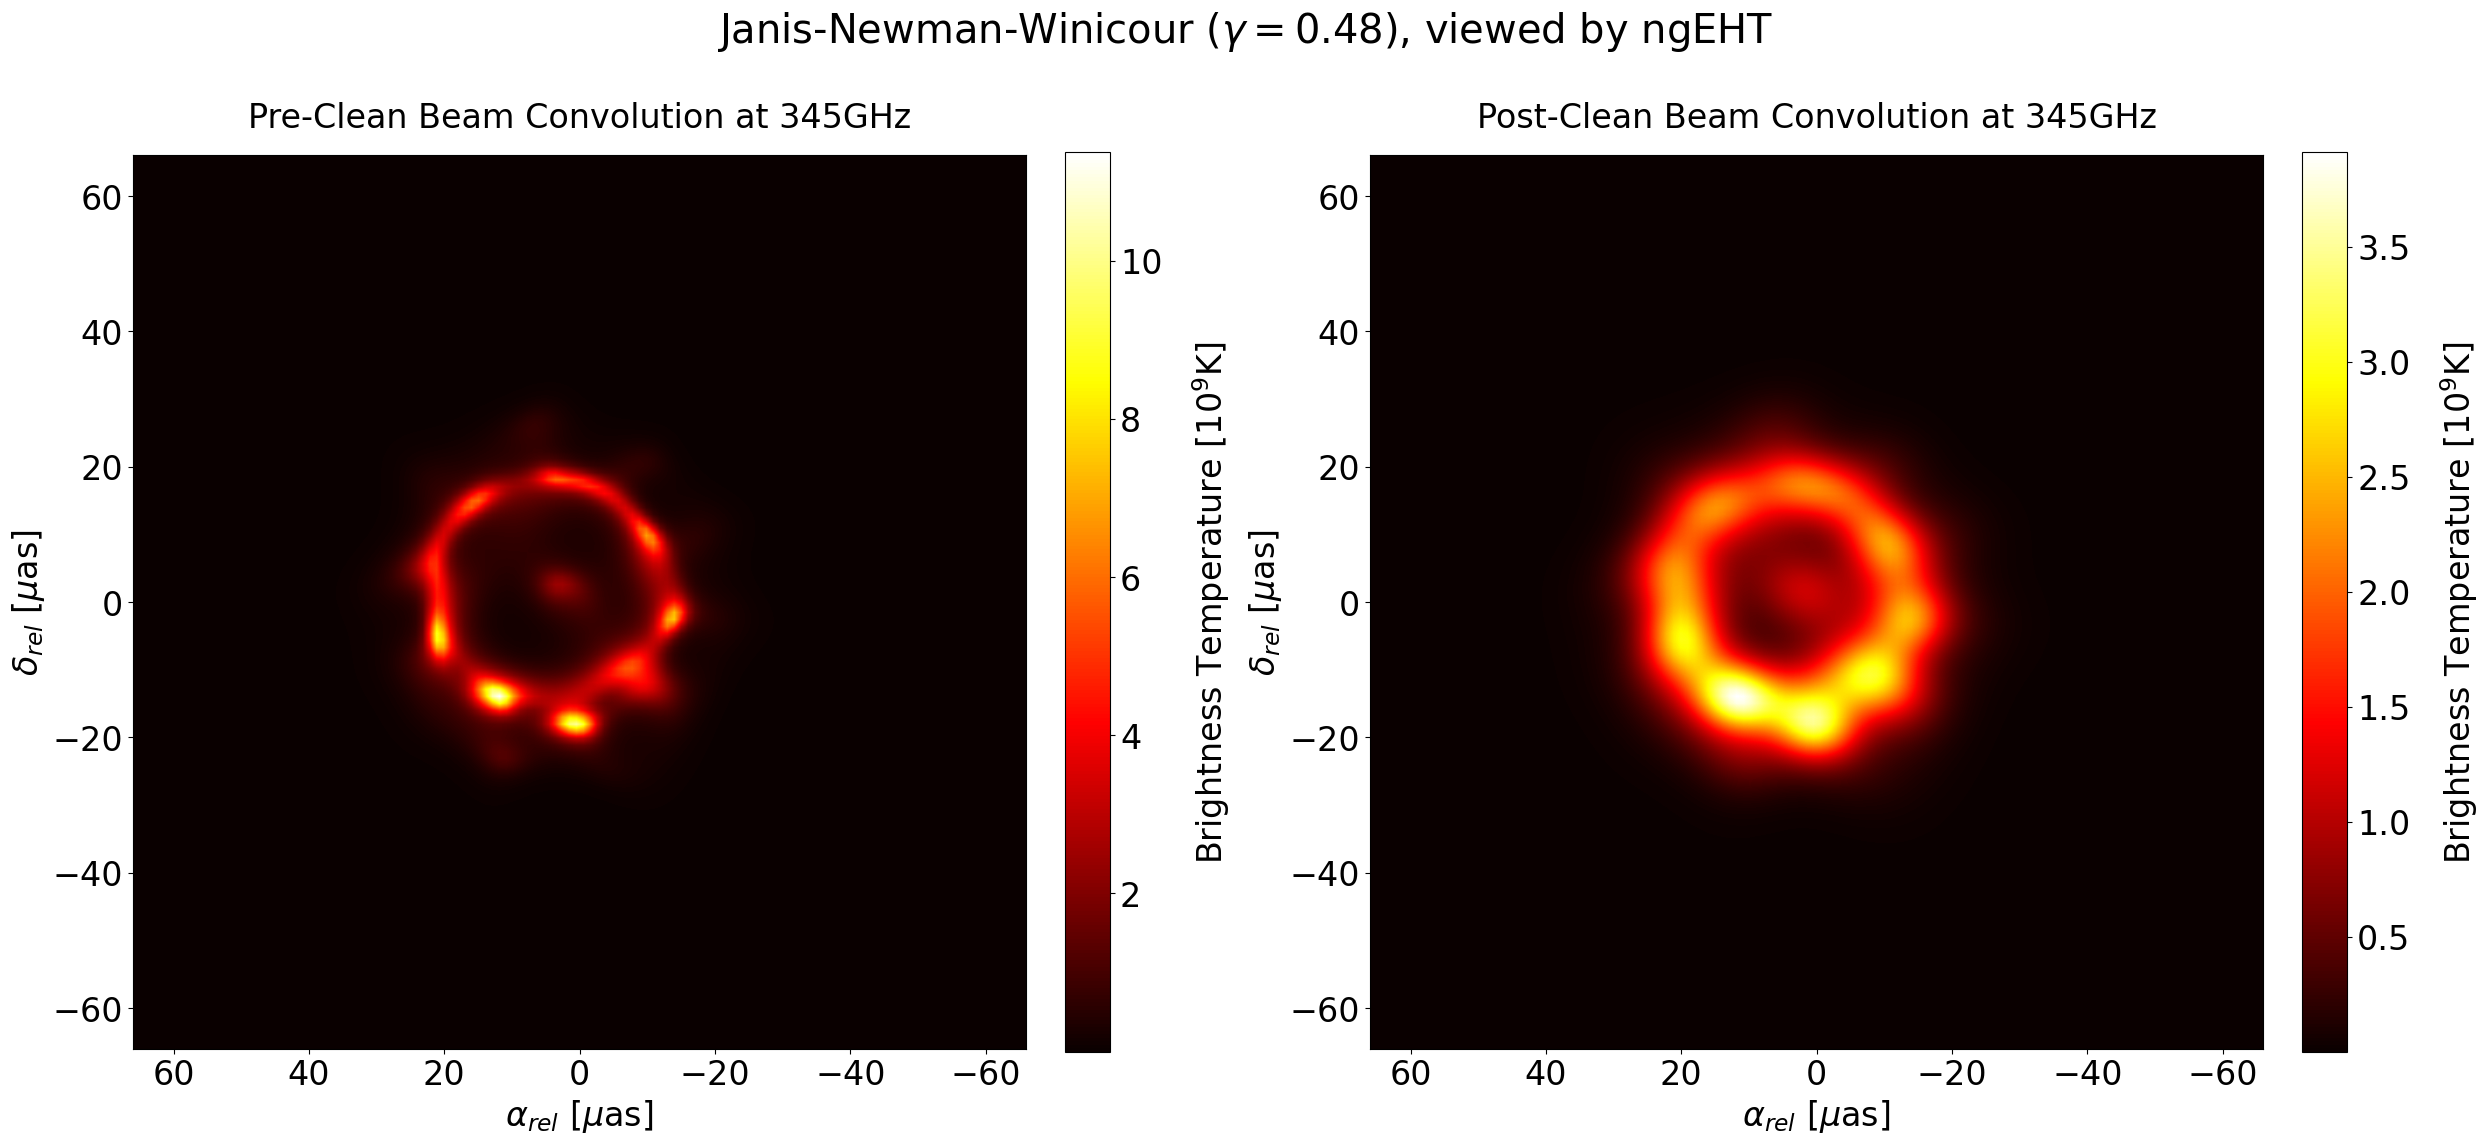
\includegraphics[scale = 0.23]{Section_8_Observing_Horizonless_Objects/Ehtim_plot_ngEHT_no_blur_345_JNW.png}
		\end{subfigure}\\
		\begin{subfigure}{12cm}
			\hspace{-1.5cm}
			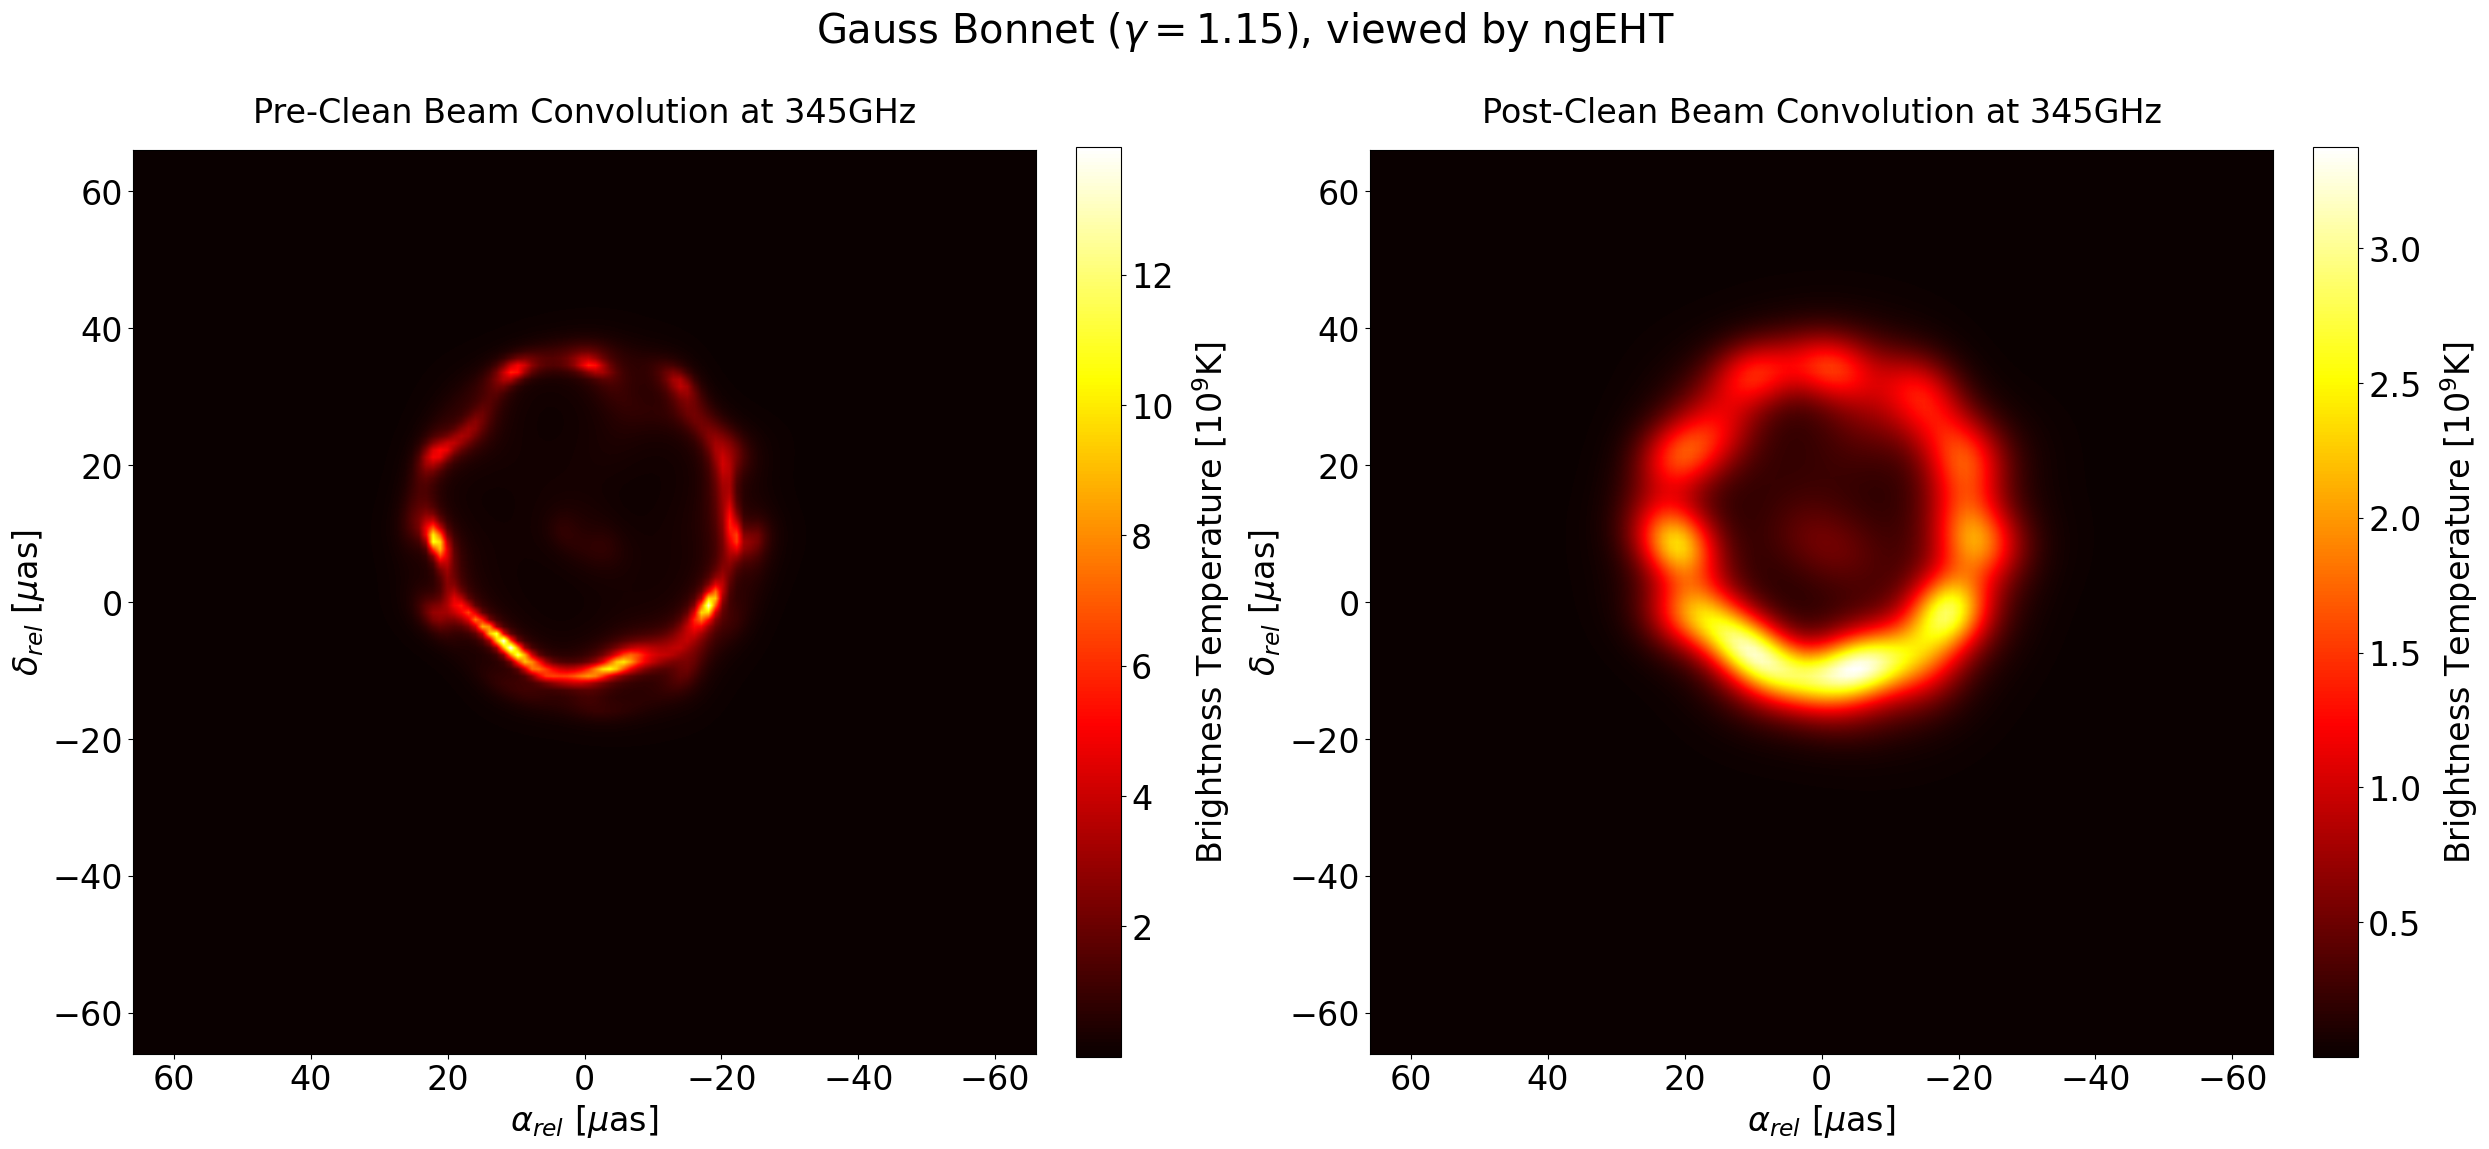
\includegraphics[scale = 0.23]{Section_8_Observing_Horizonless_Objects/Ehtim_plot_ngEHT_no_blur_345_GB.png}
		\end{subfigure}\\
		\label{Naked_Singularity_EHT_ng2017}
		\caption[Reconstructed images of naked singularities for chosen values of $\gamma$ from ngEHT.]{\small Reconstructed images of naked singularities for chosen values of $\gamma$ from ngEHT. The left panel show the "bare" reconstruction, before convolving it with the "clean beam". The final values for $\chi^2$ are $\chi^2_\text{amp} = \{1.00, 0.99\}$ and $\chi^2_\text{cl. phase} = \{1.53, 1.46\}$ for Gauss-Bonnet and Janis-Newman-Winicour respectfully.} 
	\end{figure}
	
	
	\subsection{Template analysis}
	
	To give a quantitative description of the reconstruction we need to introduce parameters which characterize their geometry. The EHT collaboration introduced for this purpose a template image of a ring with a Gaussian thickness, which they fitted to their reconstructions \cite{EHT_M87_VI}. It is characterized by a diameter, thickness and orientation. The fitted values of these are taken as the geometric properties of the reconstructions. We use a similar approach, taking advantage of the software package VIDA \cite{VIDA}. It accepts as an input a reconstructed image, to which it fits a user specified template. We choose to work with an elliptic template that has a Gaussian thickness. Details on the mathematical description of the template can be found in \cite{VIDA}, or section \emph{7.4} of the dissertation. Here we only focus on the end result of this analysis - the quantitative measure of the central depression morphology $\hat{f}_c$, defined as:
	
	\begin{equation}
		\hat{f}_c = \frac{\text{minimum flux in }\mathcal{S}}{\text{mean flux in }\mathcal{R}}.
	\end{equation}
	
	\noindent Where $\mathcal{S}$ is the central depression region, and $\mathcal{R}$ is that of the emitting ring.\\
	
	\noindent On the bottom figures we show the template analysis for the reconstructions from the 2017 EHT and ngEHT arrays. On figure 4.6 we can clearly from the sections trough the image center (the two rightmost panels) that the naked singularities show a significantly higher flux in the central depression. Using the templates generated by VIDA we calculate the measure $\hat{f}_c$ for each image in figure 4.6 and summarize them in table 3 (along with the case for a Kerr black hole with $a = 0.5$).
	
	\begin{figure}[h!]
		\centering
		\begin{subfigure}{12cm}
			\hspace{-1.5cm}
			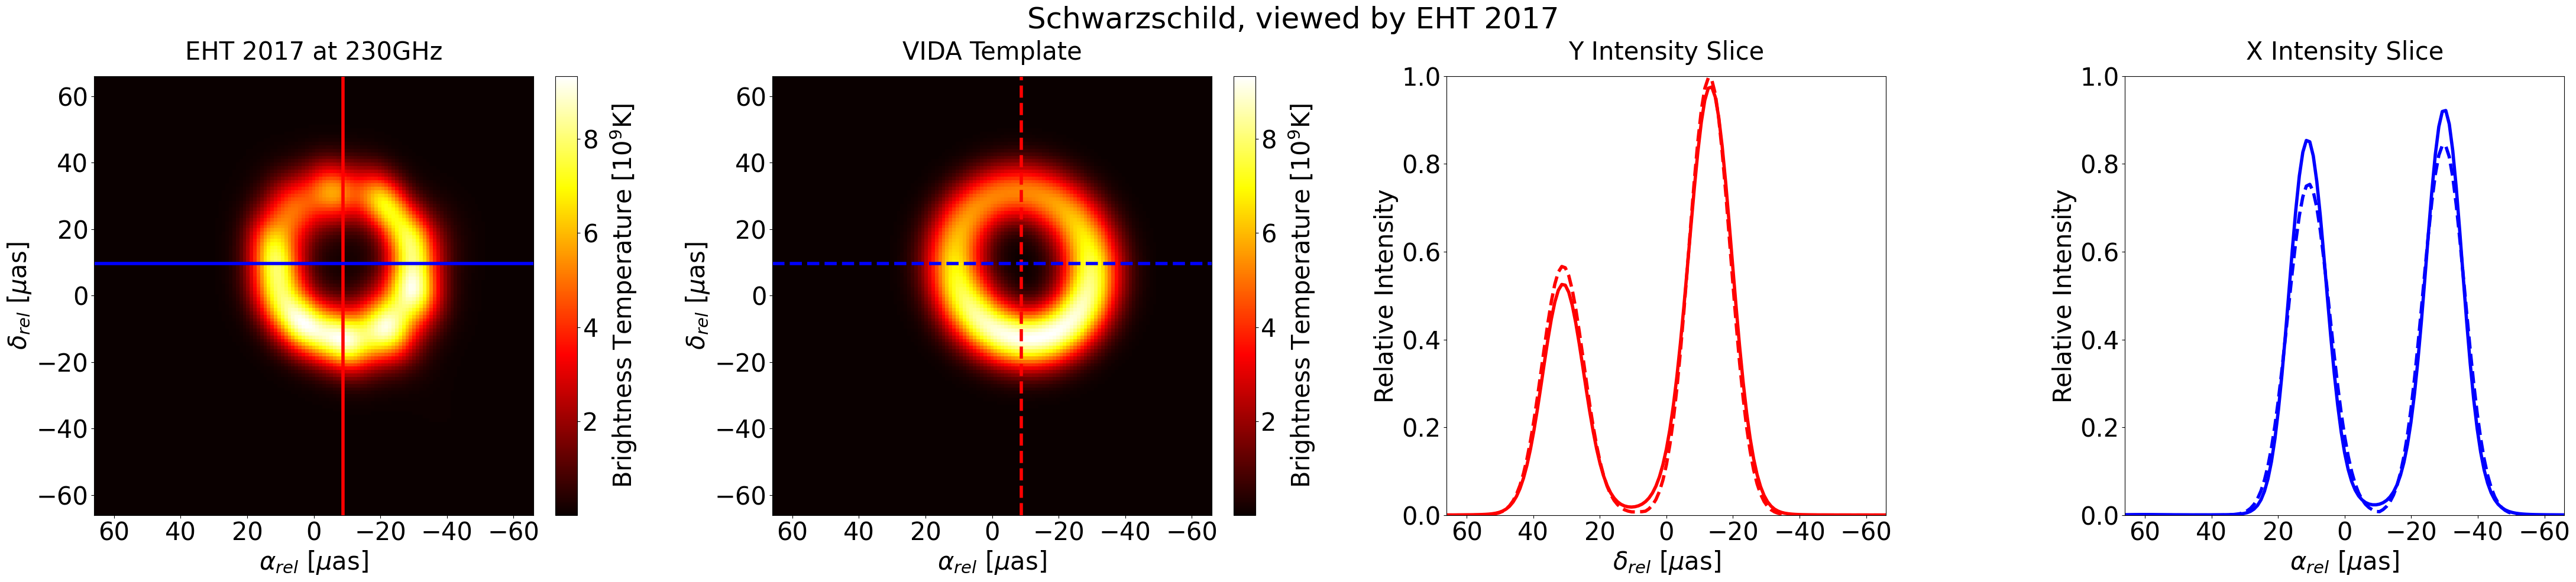
\includegraphics[scale = 0.13]{Section_8_Observing_Horizonless_Objects/Ehtim_Vida_plot_2017_230_Sch.png}
		\end{subfigure}\\
		\begin{subfigure}{12cm}
			\hspace{-1.5cm}
			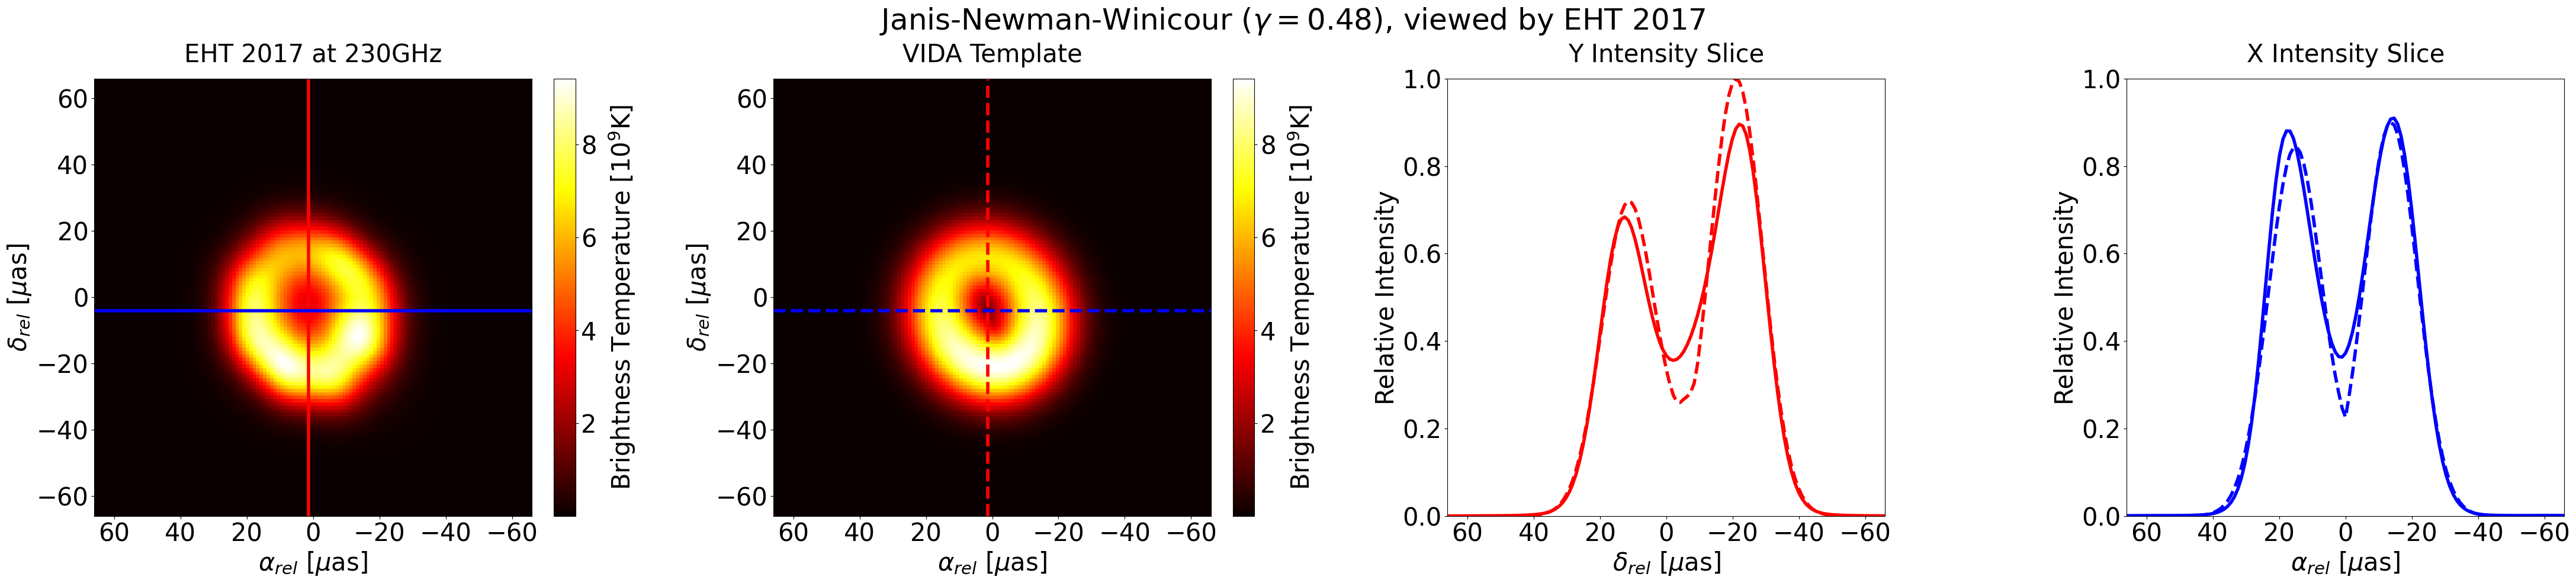
\includegraphics[scale = 0.13]{Section_8_Observing_Horizonless_Objects/Ehtim_Vida_plot_2017_230_JNW.png}
		\end{subfigure}\\
		\begin{subfigure}{12cm}
			\hspace{-1.5cm}
			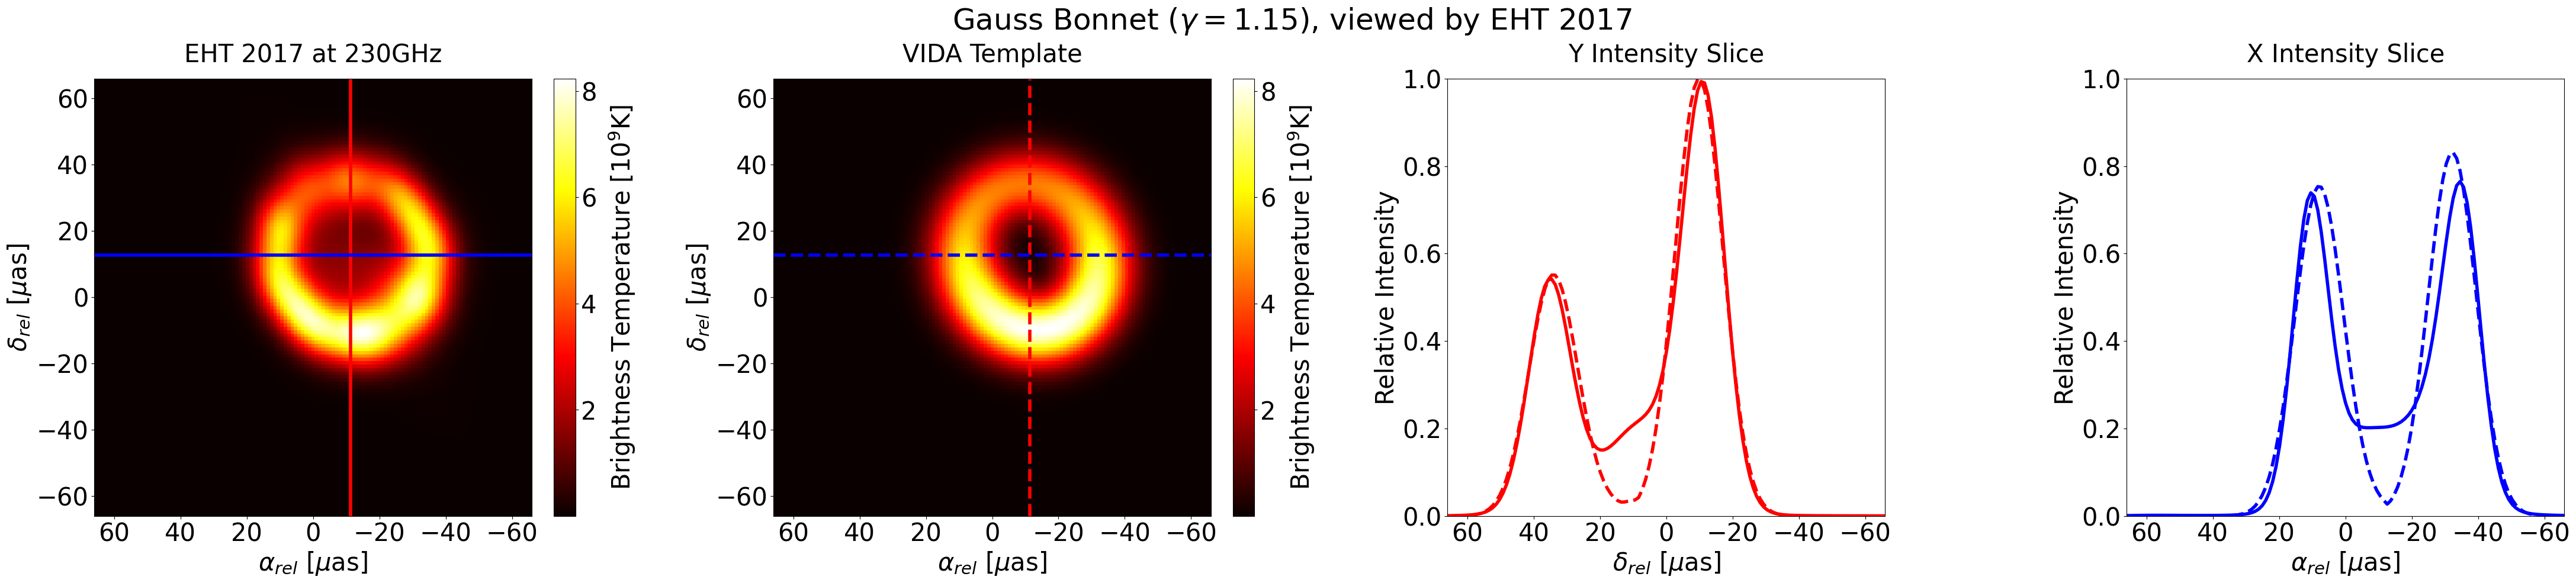
\includegraphics[scale = 0.13]{Section_8_Observing_Horizonless_Objects/Ehtim_Vida_plot_2017_230_GB.png}
		\end{subfigure}\\
		\label{VIDA_EHT_ng2017}
		\caption[Template analysis of the reconstructions from EHT 2017.]{\small Template analysis of the reconstructions from EHT 2017. On the two rightmost panels we show the vertical and horizontal intensity profile for both images trough the center $(x_0,y_0)$.} 
	\end{figure}
	
	\begin{table}[h!]
		\centering
		\begin{tabular}{||c|c|c|c|c||}
			\hline
			{Metric} & {Schwarzschild}&{Kerr (a=0.5)}&{Gauss-Bonnet}&{J.N.W.}
			\\\hline
			{\thead{$\hat{f}_c$}} & 0.026&0.030&0.239&0.451
			\\\hline
		\end{tabular}
		\caption[The qualitative measure $\hat{f}_c$ for the morphology of the central depression of EHT 2017.]{\small The qualitative measure $\hat{f}_c$ for the morphology of the central depression of EHT 2017. For comparison we also calculate the value of $\hat{f}_c$ for Kerr black holes.}
		\label{table:f_2017}
	\end{table}
	
	\newpage
	We see that the value of $\hat{f}_c$ is higher by an order of magnitude for the naked singularities. This shows that even though we cannot observationally resolve the central ring structure, the reconstructions are never the less sensitive to them, and they leave an imprint in the final image\footnote{Here one needs to be careful - the measure $\hat{f}_c$ will depends strongly on the reconstruction algorithm. Given the sparse sampling of the $(u,v)$ plane, different algorithms can give significantly different results. We would thus want the measure $\hat{f}_c$ to differ with Kerr black holes by at least \emph{two} orders of magnitude in order to take it as a sign for an unresolved central ring structure.}. On figure 4.7 we then see clearly the emergence of a central local maximum, which is due to the central ring structure. We use the templates to isolate this maximum and analyze its morphology. On figure 4.8 we show isoflux contours of the central depression of the reconstructions of the naked singularities from figure 4.2. We have compared the observations at the two frequencies $\nu = \{230, 345\}$ GHz, as well as their superposition (the leftmost panel). We observe that at 345 GHz the central maxima reach a relative intensity of $15\%$ for the Gauss-Bonnet naked singularity, and $\approx 30\%$ the Janis-Newman-Winicour one. With this we show that the central ring structure in figure 4.2 becomes extremely observationally relevant, especially at the higher frequency of 345 GHz. 
	
	\begin{figure}[h!]
		\centering
		\begin{subfigure}{12cm}
			\hspace{-1.5cm}
			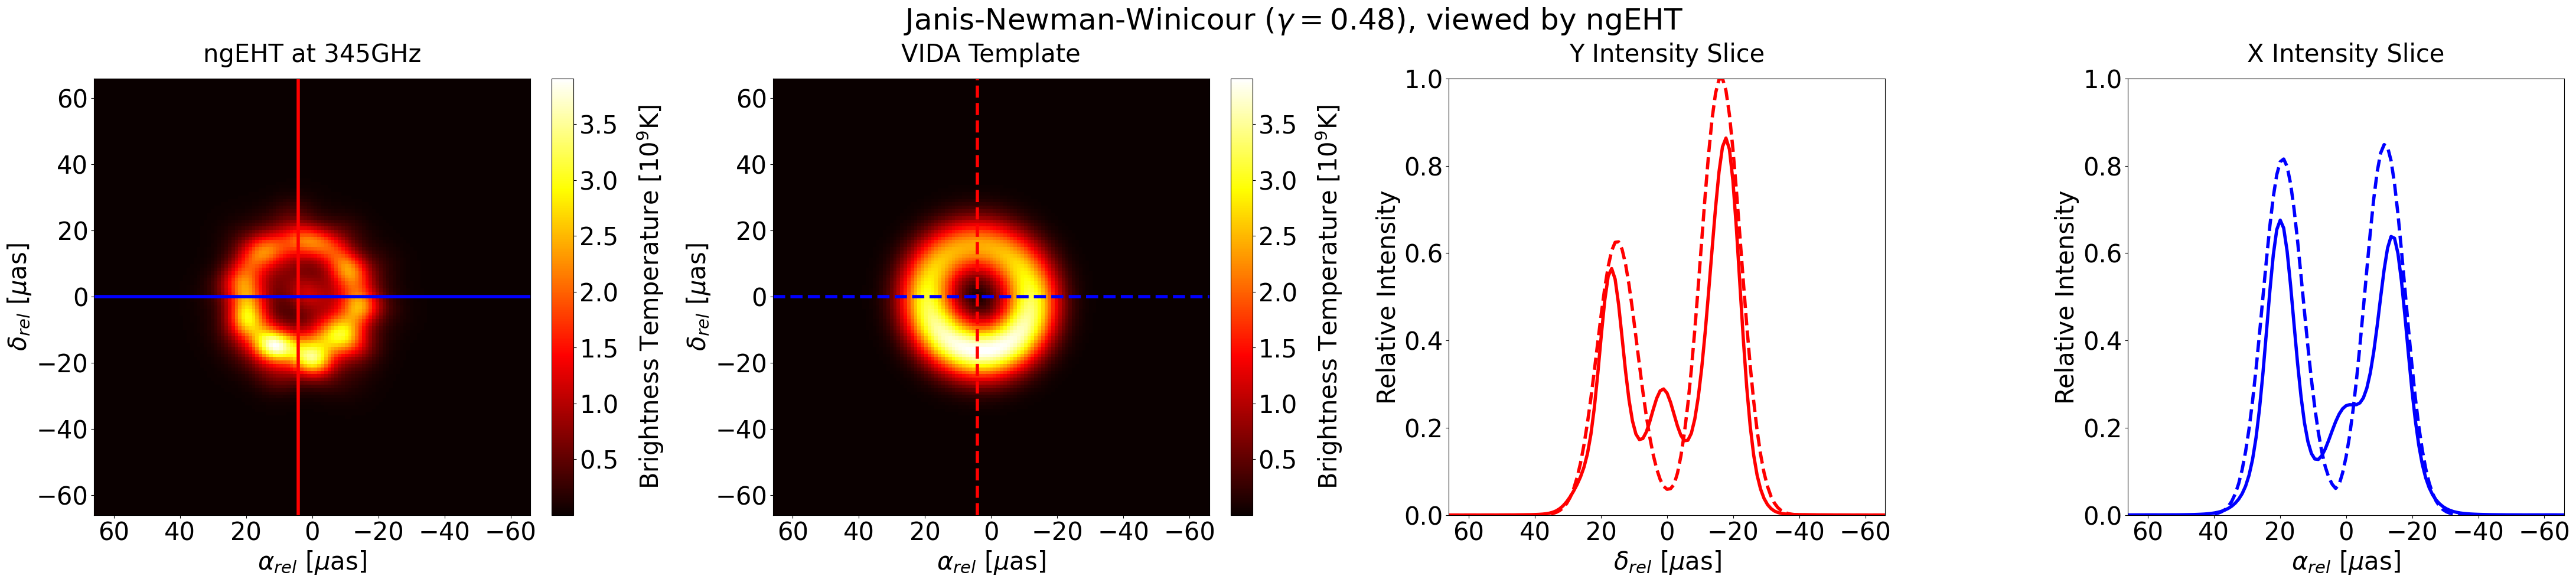
\includegraphics[scale = 0.13]{Section_8_Observing_Horizonless_Objects/Ehtim_Vida_plot_ngEHT_345_JNW.png}
		\end{subfigure}\\
		\begin{subfigure}{12cm}
			\hspace{-1.5cm}
			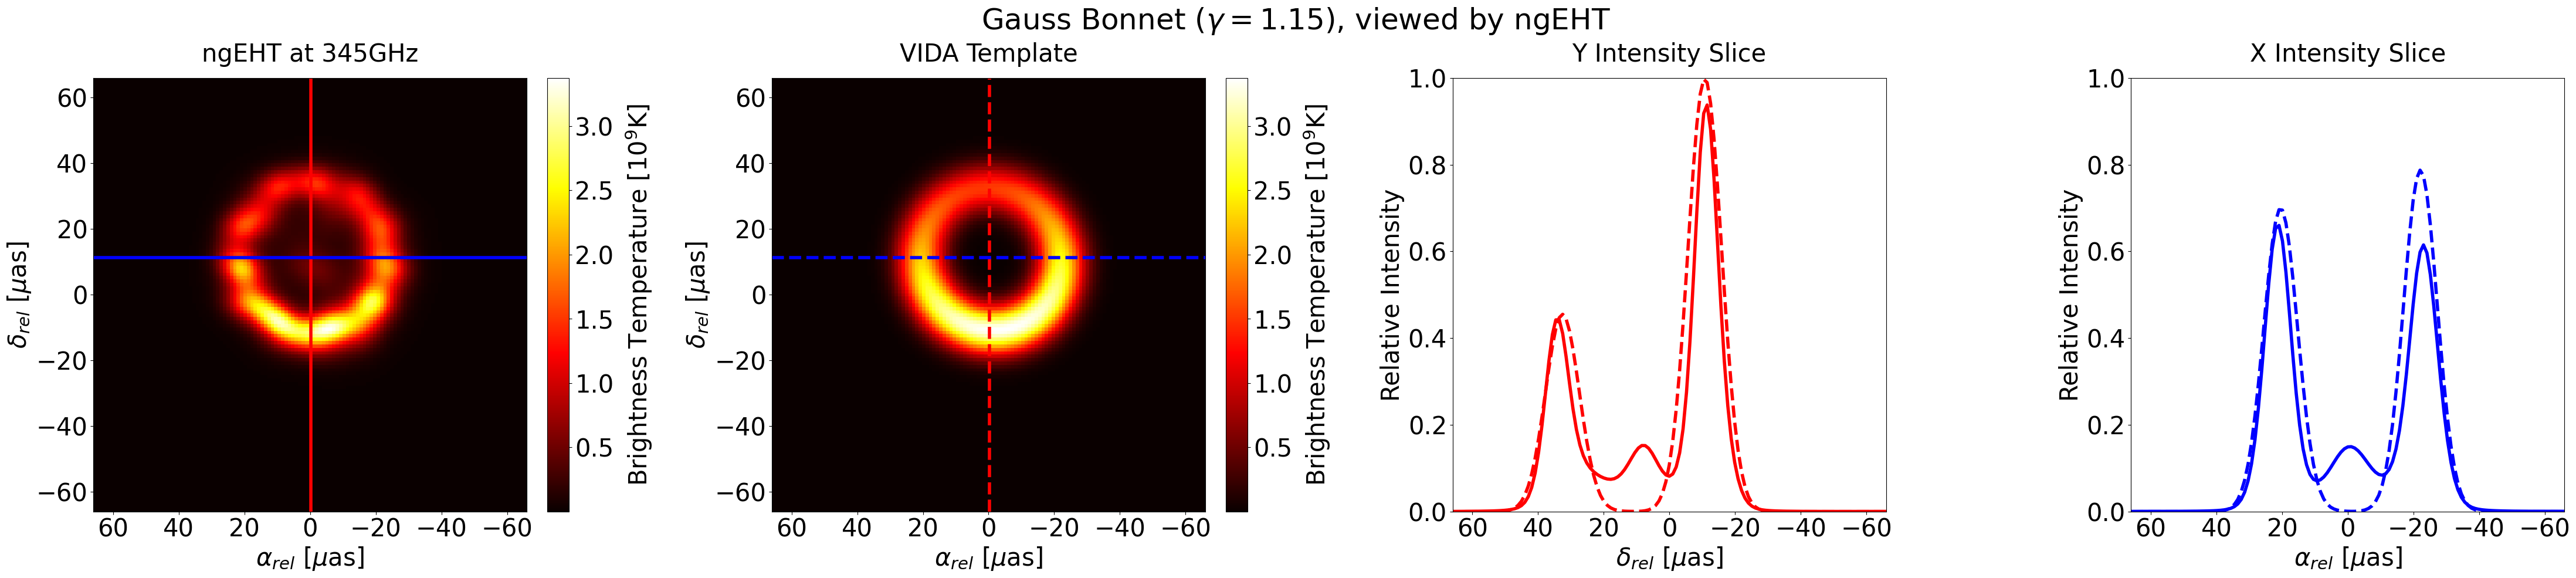
\includegraphics[scale = 0.13]{Section_8_Observing_Horizonless_Objects/Ehtim_Vida_plot_ngEHT_345_GB.png}
		\end{subfigure}\\
		\label{VIDA_ngEHT_230}
		\caption[Template analysis of the reconstructions from ngEHT at $\nu= 345$ GHz.]{\small Template analysis of the reconstructions from ngEHT at $\nu= 345$ GHz. On the two rightmost panels we show the vertical and horizontal intensity profile for both images trough the center $(x_0,y_0)$.} 
	\end{figure}
	
	\begin{table}[h!]
		\centering
		\begin{tabular}{||c|c|c|c|c||}
			\hline
			{Metric} & {Schwarzschild}&{Kerr (a=0.5)}&{Gauss-Bonnet}&{J.N.W.}
			\\\hline
			{\thead{$\hat{f}_c$ 230 GHz}} & 0.007&0.007&0.21&0.354
			\\\hline
			{\thead{$\hat{f}_c$ 345 GHz}} & 0.002&0.002&0.12&0.220
			\\\hline
			{\thead{$\hat{f}_c$ 230 GHz $\cup$ 345 GHz}} & 0.005&0.005&0.20&0.344
			\\\hline
		\end{tabular}
		\caption[The quantitative measure $\hat{f}_c$ of the morphology of the central depression for ngEHT.]{\small The quantitative measure $\hat{f}_c$ of the morphology of the central depression for ngEHT.}
		\label{table:f_ngEHT}
	\end{table}
	
	\begin{figure}[h!]
		\centering
		\begin{subfigure}{12cm}
			\hspace{-1.5cm}
			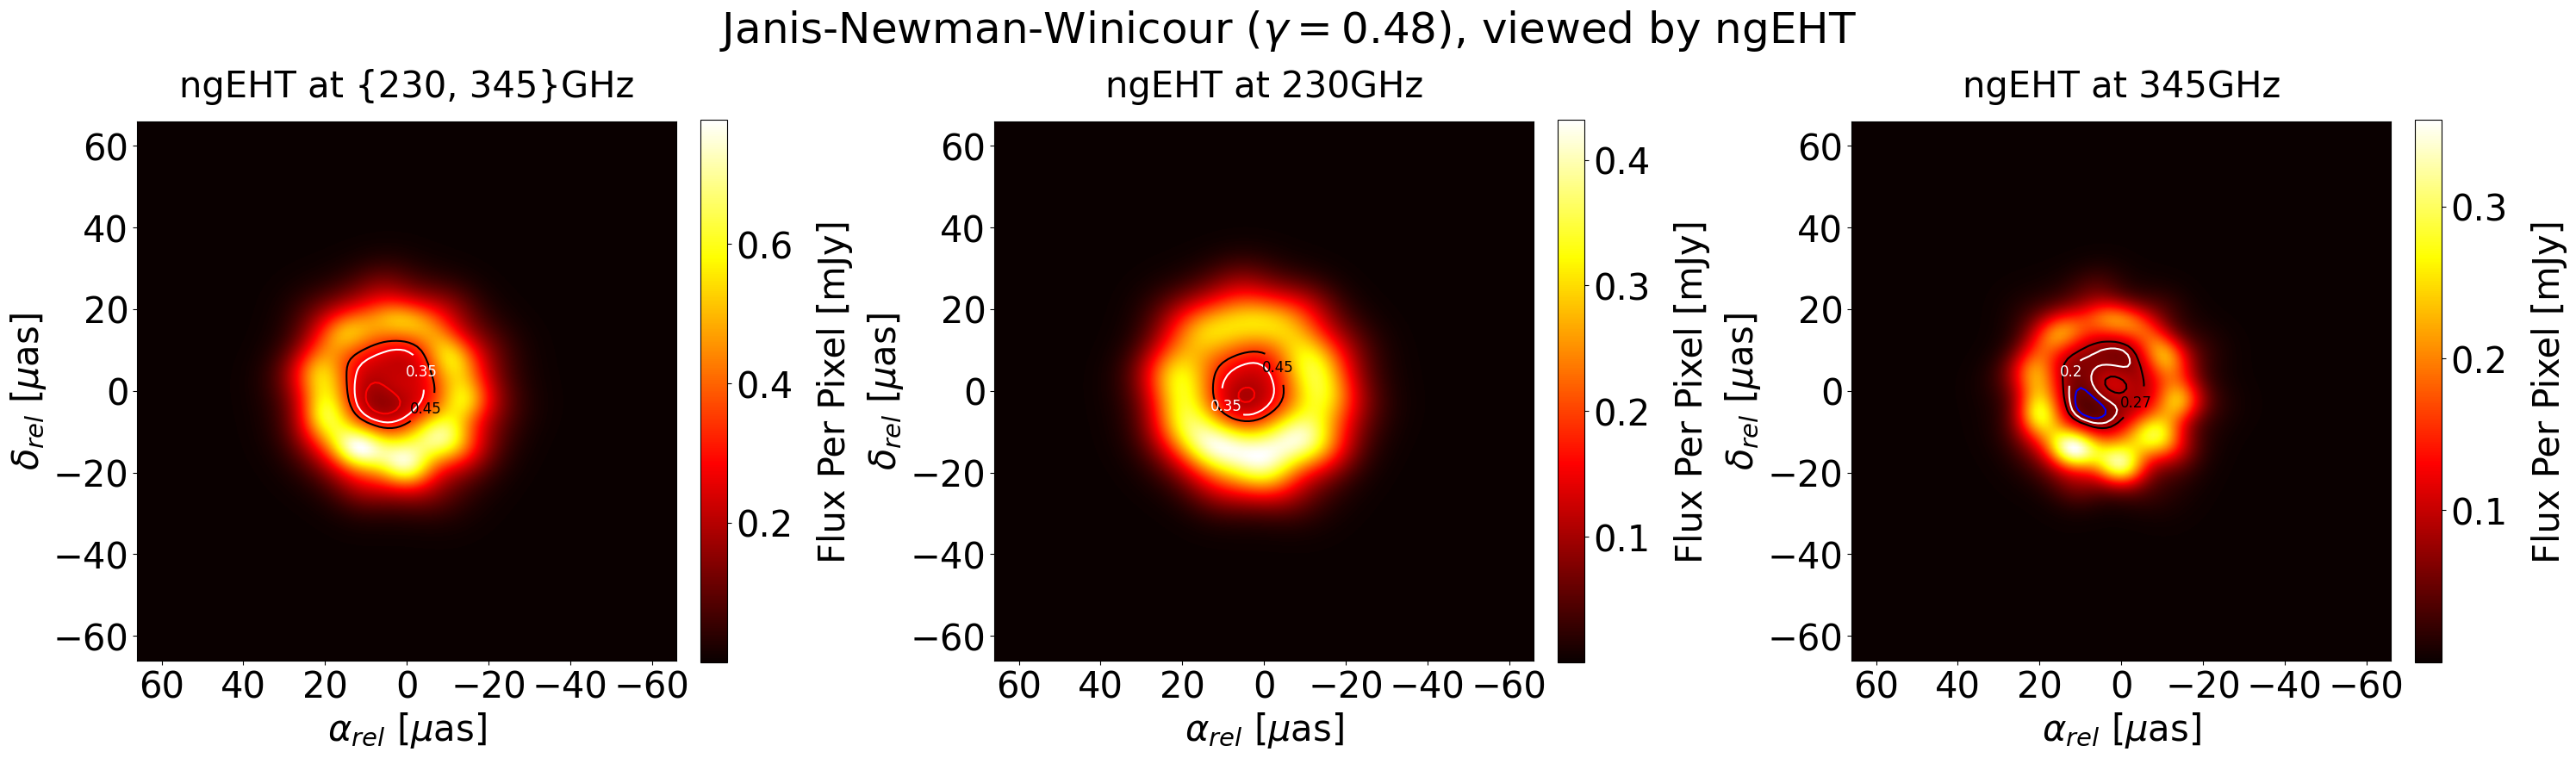
\includegraphics[scale = 0.2]{Section_8_Observing_Horizonless_Objects/Superpos_Compare_JNW.png}
		\end{subfigure}\\
		\begin{subfigure}{12cm}
			\hspace{-1.5cm}
			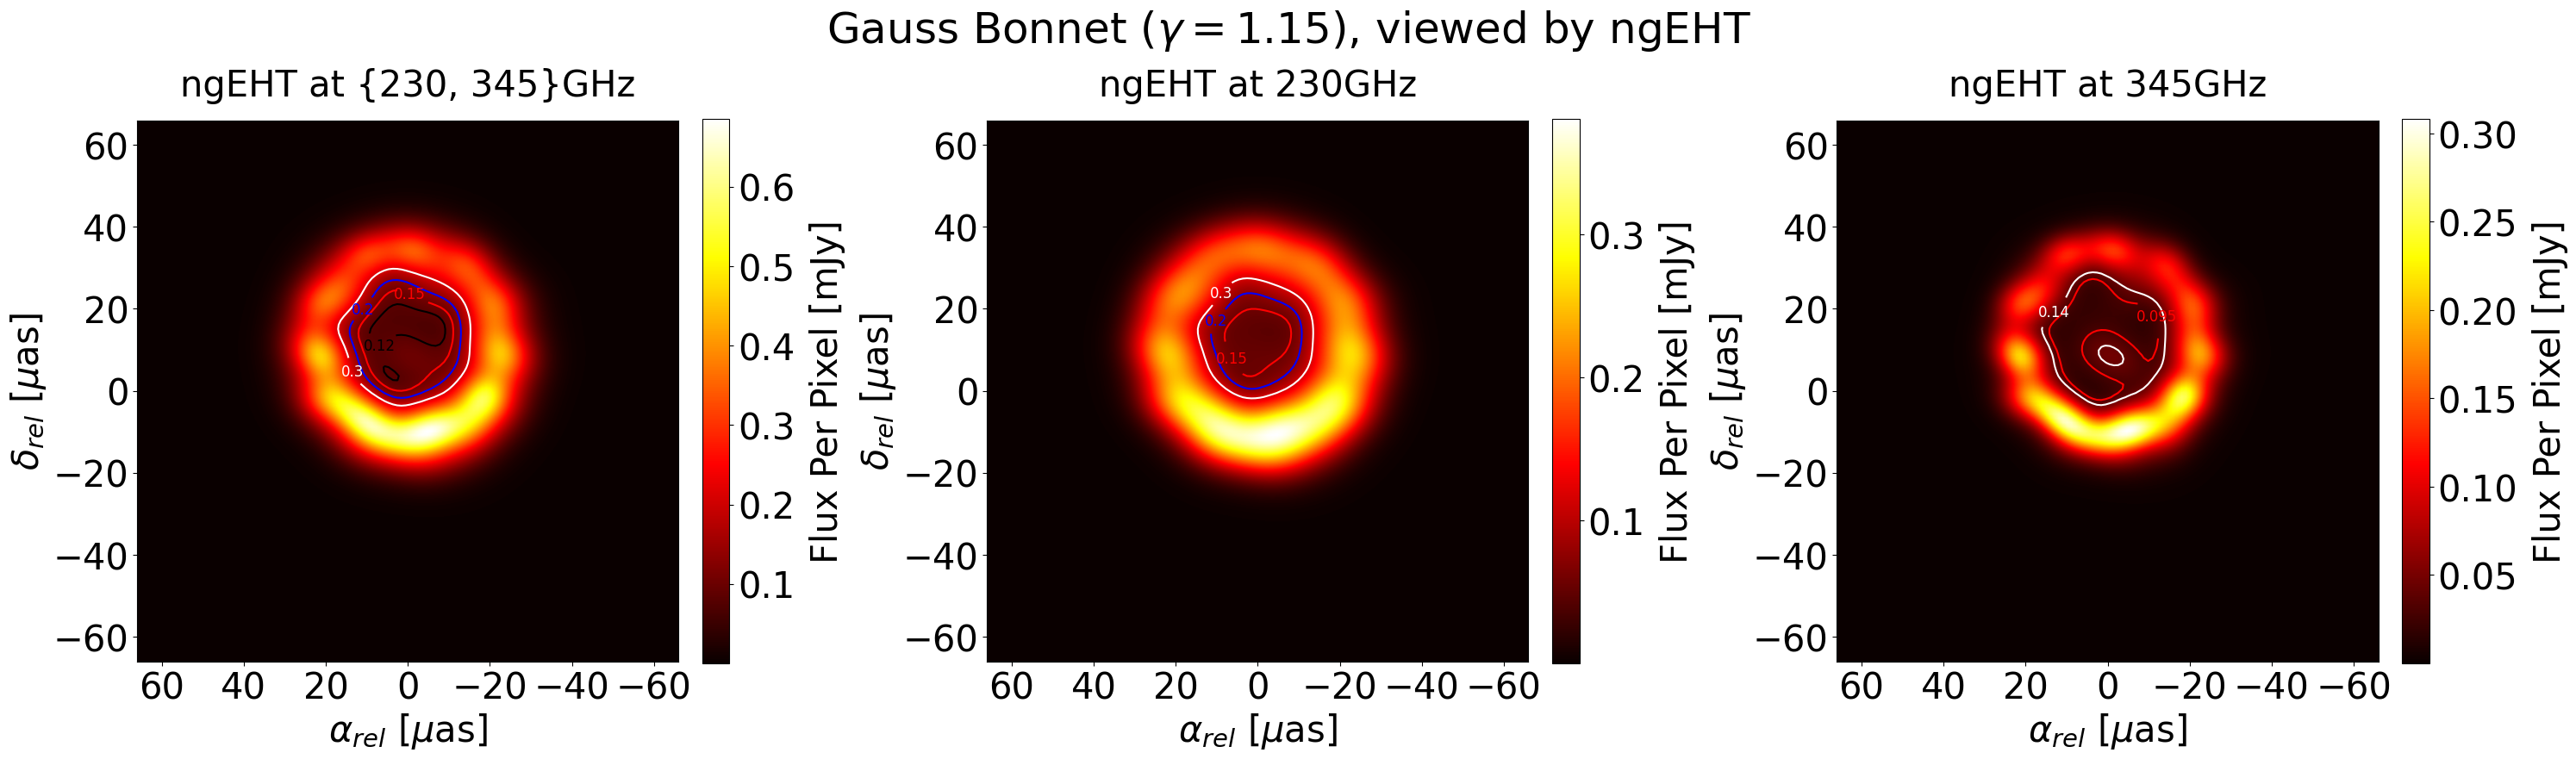
\includegraphics[scale = 0.2]{Section_8_Observing_Horizonless_Objects/Superpos_Compare_GB.png}
		\end{subfigure}\\
		\label{isoflux_ngEHT}
		\caption[Isoflux contours of the reconstruction of naked singularities from ngEHT.]{\small Isoflux contours of the reconstruction of naked singularities from ngEHT. The labels represent relative flux.} 
	\end{figure}
	
	\section{Conclusion and summary of the scientific contributions}
	
	In this dissertation we considered extensively the observational signature of two types of exotic compact objects which do not posses an event horizon - wormholes and naked singularities. Our goes was to answer the following question:\\
	
	\emph{Is it possible to distinguish such exotic compact objects from black holes via the current and future observational campaigns of the EHT collaboration?}\\
	
	We began our study with the morphology of the relativistic images, produced by these objects. In publication I (chapter \emph{5} of the dissertation and chapter \emph{2} of this abstract) we use a semi-analytic approach to generate the images of single orbits around these objects. We show that they both exhibit a qualitatively different morphology of their images, compared to Schwarzschild black holes. They form a central ring-like structure inside what would be the shadow region for a black hole. This structure corresponds to (in the case of wormholes) to photons, which pass trough the throat and (in the case of naked singularities) photons that scatter off the singularity itself. Observing such a structure will be a clear sign for the existence of such exotic spacetimes.\\
	
	Motivated by the recently published results on the linear polarization, detected by the EHT collaboration \cite{EHT_M87_VII}, \cite{EHT_M87_VIII}, we studied the imprint on the spacetime on these polarized images, as measured by a distant observer. To do this, in publications II and III we use a simplified model of the emission region \cite{Narayan2021}, generalized for arbitrary static and spherically symmetric spacetimes. The model requires the evaluation of the photon wave vector at the point of emission, which we do with the numerical code Mjølnir. Using this model we make the following conclusions for the compact objects we consider:\\
	
	\emph{1) The direct images of the emission medium are weakly influenced by the nature of the ambient spacetime. The dominating factor, determining their polarized properties is the magnetic field.}\\
	
	\emph{2) The indirect polarized images are strongly influenced by both the spacetime and the magnetic field.}\\
	
	Having this result in mind we turn our attention in publication IV (chapter \emph{7} of the dissertation and chapter \emph{4} of this abstract) to the possibility of observing the $n=1$ images, as well as the exotic ones, presented in publication I and \cite{Gyulchev2020}\cite{Gyulchev2021}. To this end we used the following software packages:\\
	
	\textbf{1)} The original code Mjølnir. In it we have implemented a model of the emission medium and we use it to generate the "ideal" images of compact objects (see appendix B of the dissertation).\\
	
	\textbf{2)} The package ehtim \cite{EHTIM}, which has two main functionalities: simulating realistic observations (i.e. $(u,v)$ sampling of the image domain) and reconstruction of the images from said simulated observations, using the methodology of the EHT collaboration. Using it we produce the reconstructed images of two types of naked singularities for three different telescope arrays and two distinct observational frequencies.\\ 
	
	\textbf{3)} The package VIDA \cite{VIDA}, which fits geometric templates to images it receives as an input. We use it to model the images generated by ehtim as ellipses with a Gaussian thickness. In this way we give geometric characteristic to the ehtim reconstructions, on which we base our conclusions.\\
	
	We show that even by expanding the telescope array compared to the 2017 EHT campaign, observations at 230 GHz cannot resolve neither the central ring structure, nor the $n = 1$ images. The reconstructions remain morphologically similar to black holes (i.e. an asymmetric emitting ring with a pronounced central depression). We observe that this central depression show a significantly heightened flux. To quantify it we introduce the measure $\hat{f}_c$, which represent the ratio between the minimum flux in the depression to the mean of the emitting ring. We find that it differs between naked singularities and black holes by an order of magnitude for the 2017 EHT array. We also see that this difference increases when we consider expanded telescope arrays.\\
	
	The more notable result is that if we increase the observational frequency to that planned by the ngEHT - 345 GHz, the reconstructions become sensitive to the central ring structure. We observe a local maximum appearing inside the central depression, whose relative intensity can reach 30\% of the image maximum. This is a characteristic morphological signature that, if observed, can serve as an indication for the existence of exotic compact objects.
	
	\section{List of the scientific activities of the author}
	
	This dissertation is based on three accepted publications, and one (as of the date of writing) in the process of approval. They are labeled with roman numbers (I, II, III and IV) in the text. Here we present a list of them.
	
	\subsection{List of scientific publications}
	
	$\bullet$ Publication I - V Deliyski, G Gyulchev, P Nedkova, and Yazadjiev. Observational features of thin accretion disks around traversable wormholes. Journal of Physics: Conference Series, 2255(1):012002, apr 2022.\\
	
	\noindent$\bullet$ Publication II - Valentin Deliyski, Galin Gyulchev, Petya Nedkova, and Stoytcho Yazadjiev. Polarized image of equatorial emission in horizonless spacetimes. Traversable wormholes. Phys. Rev. D, 106:104024, Nov 2022.\\
	
	\indent$\circ$ It is also featured in Physics Synopsis - https://physics.aps.org/articles/v15/s154\\
	
	\noindent$\bullet$ Publication III - Valentin Deliyski, Galin Gyulchev, Petya Nedkova, and Stoytcho Yazadjiev. Polarized image of equatorial emission in horizonless spacetimes: Naked singularities. Phys. Rev. D, 108:104049, Nov 2023.\\
	
	\noindent$\bullet$ Publication IV - Valentin Deliyski, Galin Gyulchev, Petya Nedkova, and Stoytcho Yazadjiev. Observing naked singularities by the present and next-generation event horizon telescope. http://arxiv.org/abs/2401.14092, 2024.
	
	\subsection{List of talks given}
	
	$\bullet$ A talk at the "National forum for contemporary space studies 2021" on the topic "Observational signatures of ultra-compact objects with accretion disks", presented on 08.10.2021\\
	
	\noindent$\bullet$ A talk given during a visit at the Emmy Noether Research Group: Gravitational waves from compact objects, Eberhard Karl university, Tuebingen, Germany, presented on 07.03.2024.\\
	
	\noindent$\bullet$ A talk given at the Seventeenth Marcel Grossman Meeting on the topic "Polarized image of equatorial emission in horizonless spacetimes".
	
	\newpage
	
	\bibliographystyle{unsrt}
	\bibliography{References}
\end{document}